\chapter{Beyond Leading Log with High Energy Jets}

Now that the driving principles behind HEJ have been explained, we move on to discuss the recent improvements to the formalism. We begin by discussing how the form of our amplitudes allows us to also capture terms which are Next-to-Leading Log (NLL) in the perturbative series. We will go into the motivations for why we should do this before presenting a full description of how some of these terms are derived and incorporated. We then finalise the chapter by presenting new results clearly showing the effect of the addition of these contributions, both in terms of the HEJ program and in comparison to real LHC data. 

\section{Motivations for NLL}

There are a few reasons one might consider trying to go beyond Leading Log with the formalism. Firstly, since it has been proved that the Lipatov ansatz is valid at the NLL level \cite{Fadin2006}, any sub-leading amplitude that still factors out into a product of $t$-channel poles can be resummed in precisely the same way as before; there is no added complication to the resummation procedure itself. The formalism thus lends itself naturally and readily to this extension. Secondly, by having access to these sub-leading terms we also expect to reduce the scale variation bands on our calculation, since these variations are directly related to how much `control' we have over higher order terms. In order to claim full NLL accuracy, we must have;

\begin{enumerate}
\item{Calculations of FKL amplitudes but with the rapidity ordering of one emitted gluon disturbed. We call such contributions `unordered' processes.}
\item{Corrections to the Lipatov vertex for the emission of gluons.}
\item{Calculations of inherently non-FKL amplitudes that appear at the NLL level.}
\end{enumerate}

%\todo{talk more about uno here}
The first point had already been implemented in theory but had not been incorporated into the program. The second point has not yet been attempted but remains a long term goal of the collaboration. This thesis will consider the first and final points, providing a brief overview of the former and a complete description and derivation of the author's individual work for the latter. Including such considerations will mark an important step towards full NLL HEJ and, in the case of the addition of the non-FKL subprocesses, it extends the applicability of HEJ since we will now have a Leading Log description of these events; in conclusion, we will be able to resum more of the contribution to the cross section. 

\section{Unordered Emissions in Pure Jets}
%\todo{Uno section! Or incorporated into last section?}
The derivation of the amplitude for an unordered (or simply `uno') contribution revolves around extending our current formalism to include the effect of a gluon being emitted outside of the FKL strong rapidity ordered chain. We can express this by having a new `current' that depends on the rapidity of this unordered parton and the parton next to it in rapidity that satisfies the ordering. For example, the amplitude for $qQ \to gqQ$ would look something like;

\begin{equation}
M_{qQ \to gqQ}^{uno} \sim \frac{j^\mu_{uno}(p_a,p_1,p_{uno})j_\mu(p_b,p_2)}{\hat{t}_2},
\label{eqn:uno}
\end{equation}

\begin{figure}[t]
\centering
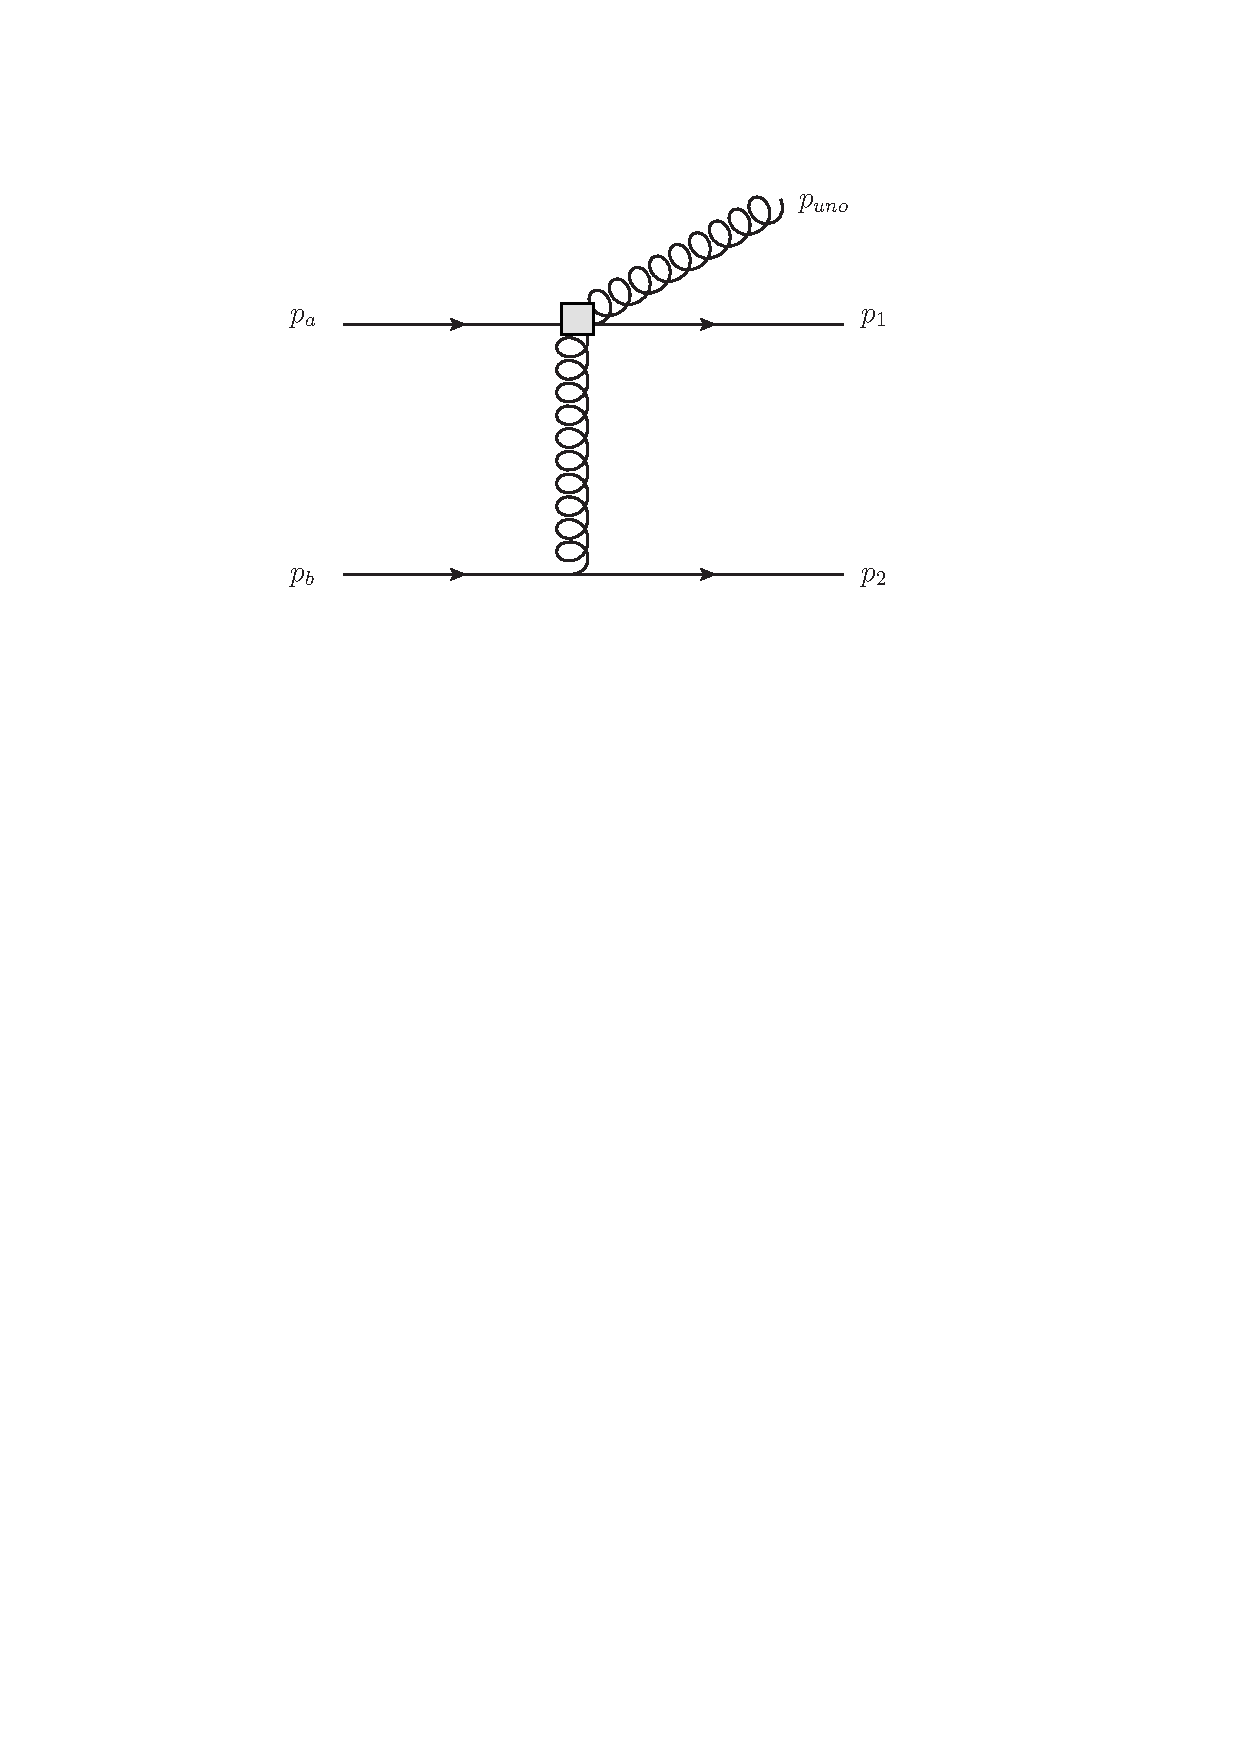
\includegraphics[scale=0.7]{Images/uno.pdf}
\caption{A schematical view of an unordered emission amplitude.}
\label{fig:uno}
\end{figure}

where $y_{uno} \sim y_1, y_1 \gg y_2$. In essence, we collapse the gluon emission to a point along the usual current such that there is only one suitable $t$-channel pole to be resummed as opposed to the two we would get if the gluon was emitted in the FKL ordering - it is thus clear to see why this is a sub-leading log contribution. Diagrammatically, we can show this like the schematic drawing in figure \ref{fig:uno}. We should also keep in mind that when it comes to discussing the colour properties of this amplitude that it will be more complicated than the FKL case and the result will have to be treated more carefully in this regard. To derive the form of the uno current, we will simply recalculate the $qQ \to gqQ$ amplitude but with the consideration that the rapidity of the gluon is no longer far away form the rapidity of the forward quark current. What this will essentially mean is that the kinematic arguments for dropping some terms like we did in section 2.2.3 will no longer be valid. We will therefore start by writing the full LO result for this amplitude (where we will write $p_{uno} = p_g$ for brevity);

\begin{equation}
\begin{split}
M_{qQ \to gqQ}^{LO} &= (ig_s)^3 T^c_{1i}T_{ia}^d T^d_{2b} \varepsilon_{\nu}(p_g) \frac{\matel{1}{\nu}{g}\matel{g}{\mu}{a} + 2p_1^\nu \matel{1}{\mu}{a}}{s_{1g}\hat{t}_2}\matel{2}{\mu}{b} \\
 &- (ig_s)^3 T^d_{1i}T_{ia}^c T^d_{2b} \varepsilon_{\nu}(p_g) \frac{2p_a^\nu \matel{1}{\mu}{a} - \matel{1}{\mu}{g}\matel{g}{\nu}{a}}{s_{ag}\hat{t}_2}\matel{2}{\mu}{b} \\
 &+ (ig_s)^3 T^c_{2i}T_{ib}^d T^d_{1a} \varepsilon_{\nu}(p_g) \frac{\matel{2}{\nu}{g}\matel{g}{\mu}{b} + 2p_2^\nu \matel{2}{\mu}{b}}{s_{2g}\hat{t}_1}\matel{1}{\mu}{a} \\
  &- (ig_s)^3 T^d_{2i}T_{ib}^c T^d_{1a} \varepsilon_{\nu}(p_g) \frac{2p_b^\nu \matel{2}{\mu}{b} - \matel{2}{\mu}{g}\matel{g}{\nu}{b}}{s_{bg}\hat{t}_1}\matel{1}{\mu}{a} \\
  &-g_s^3 f^{dec}T^d_{1a}T^e_{2b} \varepsilon_\nu(p_g) \frac{\matel{1}{\rho}{a}\matel{2}{\mu}{b}}{\hat{t}_1 \hat{t}_2}(2p_g^\mu \eta^{\nu \rho} - 2p_g^\rho \eta^{\mu \nu} - (q_1 + q_2)^\nu \eta^{\mu \rho}).
\end{split}
\end{equation}

With the full expression available, we can investigate which terms we can still drop in this new limit $y_g \sim y_1 \gg y_2$. We see that the first term in the third line and the second term in the fourth are the only ones we can drop because (depending on helicities) the $\mu$ contraction will give something that scales as $\sqrt{s_{ag}}$ or $\sqrt{s_{g1}}$ which are now small invariants in comparison to everything else. By dropping these terms, all remaining terms are proportional to $\matel{2}{\mu}{b}$ and so by comparison to equation \ref{eqn:uno}, the sum of the terms multiplying this current is what will give us our unordered current. However, to be truly consistent with the factorised picture, we must factorise out the colour factor $T^d_{2b}$ from this amplitude as well. This is already the case for the first, second and last lines and now that we have dropped terms for the other two lines we can use the still valid limit $p_2 \sim p_b$ to yield;

\begin{equation}
\begin{split}
& -ig_s^3 \matel{1}{\mu}a{} \matel{2}{\mu}{b} \varepsilon_\nu(p_g) \left(\frac{2p_2^\nu}{\hat{t}_1 s_{2g}} - \frac{2p_b^\nu}{\hat{t}_1s_{bg}} \right) \\
& \approx -i g_s^3 \matel{1}{\mu}{a} \matel{2}{\mu}{b} \varepsilon_\nu(p_g) \frac{1}{\hat{t}_1}\frac{2p_b^\nu}{s_{bg}} T^d_{1a}\left(T^c_{2i}T^d_{ib} - T^d_{2i}T^c_{ib}\right)  \\
&= g_s^3 \matel{1}{\mu}{a} \matel{2}{\mu}{b} \varepsilon_\nu(p_g) \frac{1}{\hat{t}_1} \frac{2 p_b^\nu}{s_{bg}} f^{cde}T^d_{1a}T^e_{2b} \\
&= g_s^3 \matel{1}{\mu}{a} \matel{2}{\mu}{b} \varepsilon_\nu(p_g) f^{cde}T^d_{1a}T^e_{2b} \frac{1}{\hat{t}_1} \left(\frac{p_b^\nu}{s_{bg}}+\frac{p_2^\nu}{s_{2g}} \right),
\end{split}
\end{equation}

where in the last line we have restored the symmetry between $p_2$ and $p_b$. Our factorised amplitude then looks like;

\begin{equation}
M_{qQ \to gqQ}^{uno, fact} = -g_s^3 \frac{\matel{2}{\mu}{b}}{\hat{t}_2}T_{2b}^d \left(iT^c_{1i}T^d_{ia}U_1^{\mu \nu} + iT^d_{1i}T^c_{ia}U_2^{\mu \nu} + f^{ecd}T^e_{1a}L^{\mu \nu} \right),
\end{equation}

where;
\begin{equation}
\begin{split}
U_1^{\mu \nu} &= \frac{1}{s_{1g}}(j^\nu_{1g}j^\mu_{ga} + 2 p_1^\nu j^\mu_{1a}) \\
U_2^{\mu \nu} &= -\frac{1}{s_{ag}}(2j^\mu_{1a}p_a^\nu - j^\mu_{1g}j^\nu_{ga}) \\
L^{\mu \nu} &= \frac{1}{\hat{t}_1} \left(-2p^\mu_g j^\nu_{1a} + 2 p_g \cdot j_{1a}\eta^{\mu \nu} + (q_1 + q_2)^\nu j^{\mu}_{1a} + \hat{t}_2 j^\mu_{1a} \left(\frac{p_2^\nu}{s_{2g}} + \frac{p_b^\nu}{s_{gb}} \right) \right).
\end{split}
\end{equation}

The three colour factors are not independent here, so we can combine them and then we can extract the uno current by inspection;

\begin{equation}
j^\mu_{uno}(p_1, p_a, p_g) = i \varepsilon_\nu(p_g) \left(T^c_{1i}T^d_{ia}\left(U_1^{\mu \nu} - L^{\mu \nu}\right) + T^d_{1i}T^c_{1a}\left(U_2^{\mu \nu} + L^{\mu \nu}\right) \right).
\end{equation}

Gauge invariance of this expression has been checked by replacing the polarisation vector with the gluon momentum and seeing that the expression gives zero. This current can then be used as a basis for all unordered amplitudes, with further emissions added on via the Lipatov vertex and other incoming states accounted for by colour Casamir multiplications. One thing to note, however, is that the leg that the unordered current is dependent on cannot be a gluon, since a trivial rewriting of momenta in that case will lead back to the FKL ordering. 

\section{Calculations of NLL Partonic Subprocesses}

It was discussed in chapter two that the leading amplitudes in the High Energy limit are given by those that involve the maximal number of gluon exchanges in the $t$-channel by analysis of Regge Theory. To access the sub-leading partonic configurations, we simply replace one gluon propagator by one quark propagator in these FKL amplitudes (whilst keeping the strict rapidity ordering). There are two distinct possibilities we can imagine - we can either replace the first or last propagator in the chain or one in the middle along the chain. We can assign the nomenclature `extremal' and `central' to the two cases respectively. The simplest case of an extremal process is $qg \to qQ\bar{Q}$ and for the central case it is $qq' \to qQ\bar{Q}q'$. Once we have expressions for these amplitudes in our language, we can build up all other related amplitudes by once more multiplying in Lipatov vertices and multiplying by ratios of colour factors. 

\subsection{Calculation of $qg \to qQ\bar{Q}$ in the High Energy Limit}

The ultimate aim of this calculation will be to factorise the $qg \to qQ\bar{Q}$ amplitude into an expression like;

\begin{equation}
M_{qg \to qQ\bar{Q}} \sim \frac{\matel{1}{\mu}{a}Q^{\mu \nu}(p_2, p_3, p_b) \varepsilon_\nu(p_b)}{\hat{t}_1},
\label{eqn:NLLeqn}
\end{equation}

where $Q^{\mu \nu}$ is an effective vertex that encapsulates the effect of the emission of a quark/anti-quark pair at the end of the rapidity chain. We can schematically show this equation as a diagram like in figure \ref{fig:qgimp}. Given the momentum dependence of the vertex and how it looks schematically, we can also interpret $Q^{\mu \nu}$ as a $g \to q \bar{q}$ \emph{impact factor}.

\begin{figure}[t]
\centering
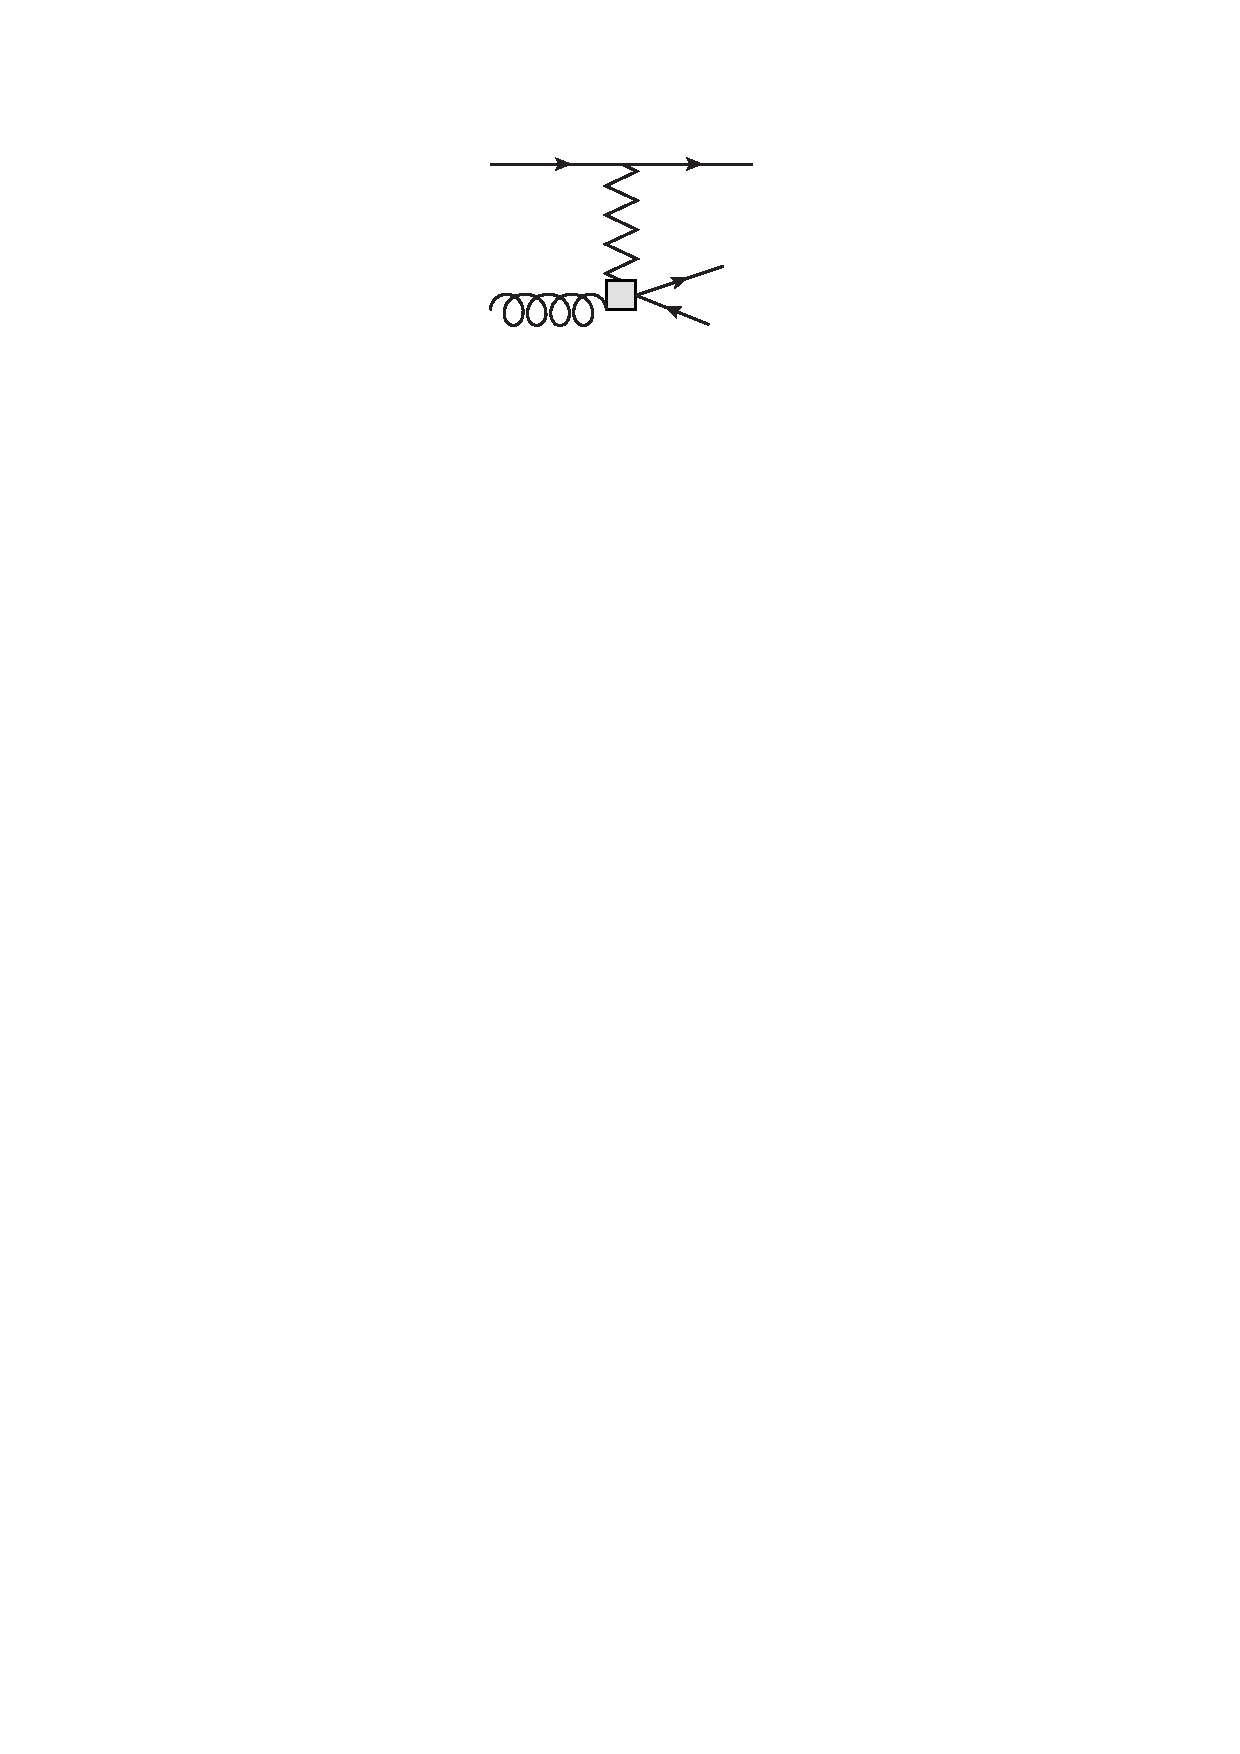
\includegraphics{Images/g_q_qbar_imp.pdf}
\caption{Schematic diagram involving $g \to q \bar{q}$ impact factor.}
\label{fig:qgimp}
\end{figure}

\begin{figure}[t] 
\centering
\subfloat{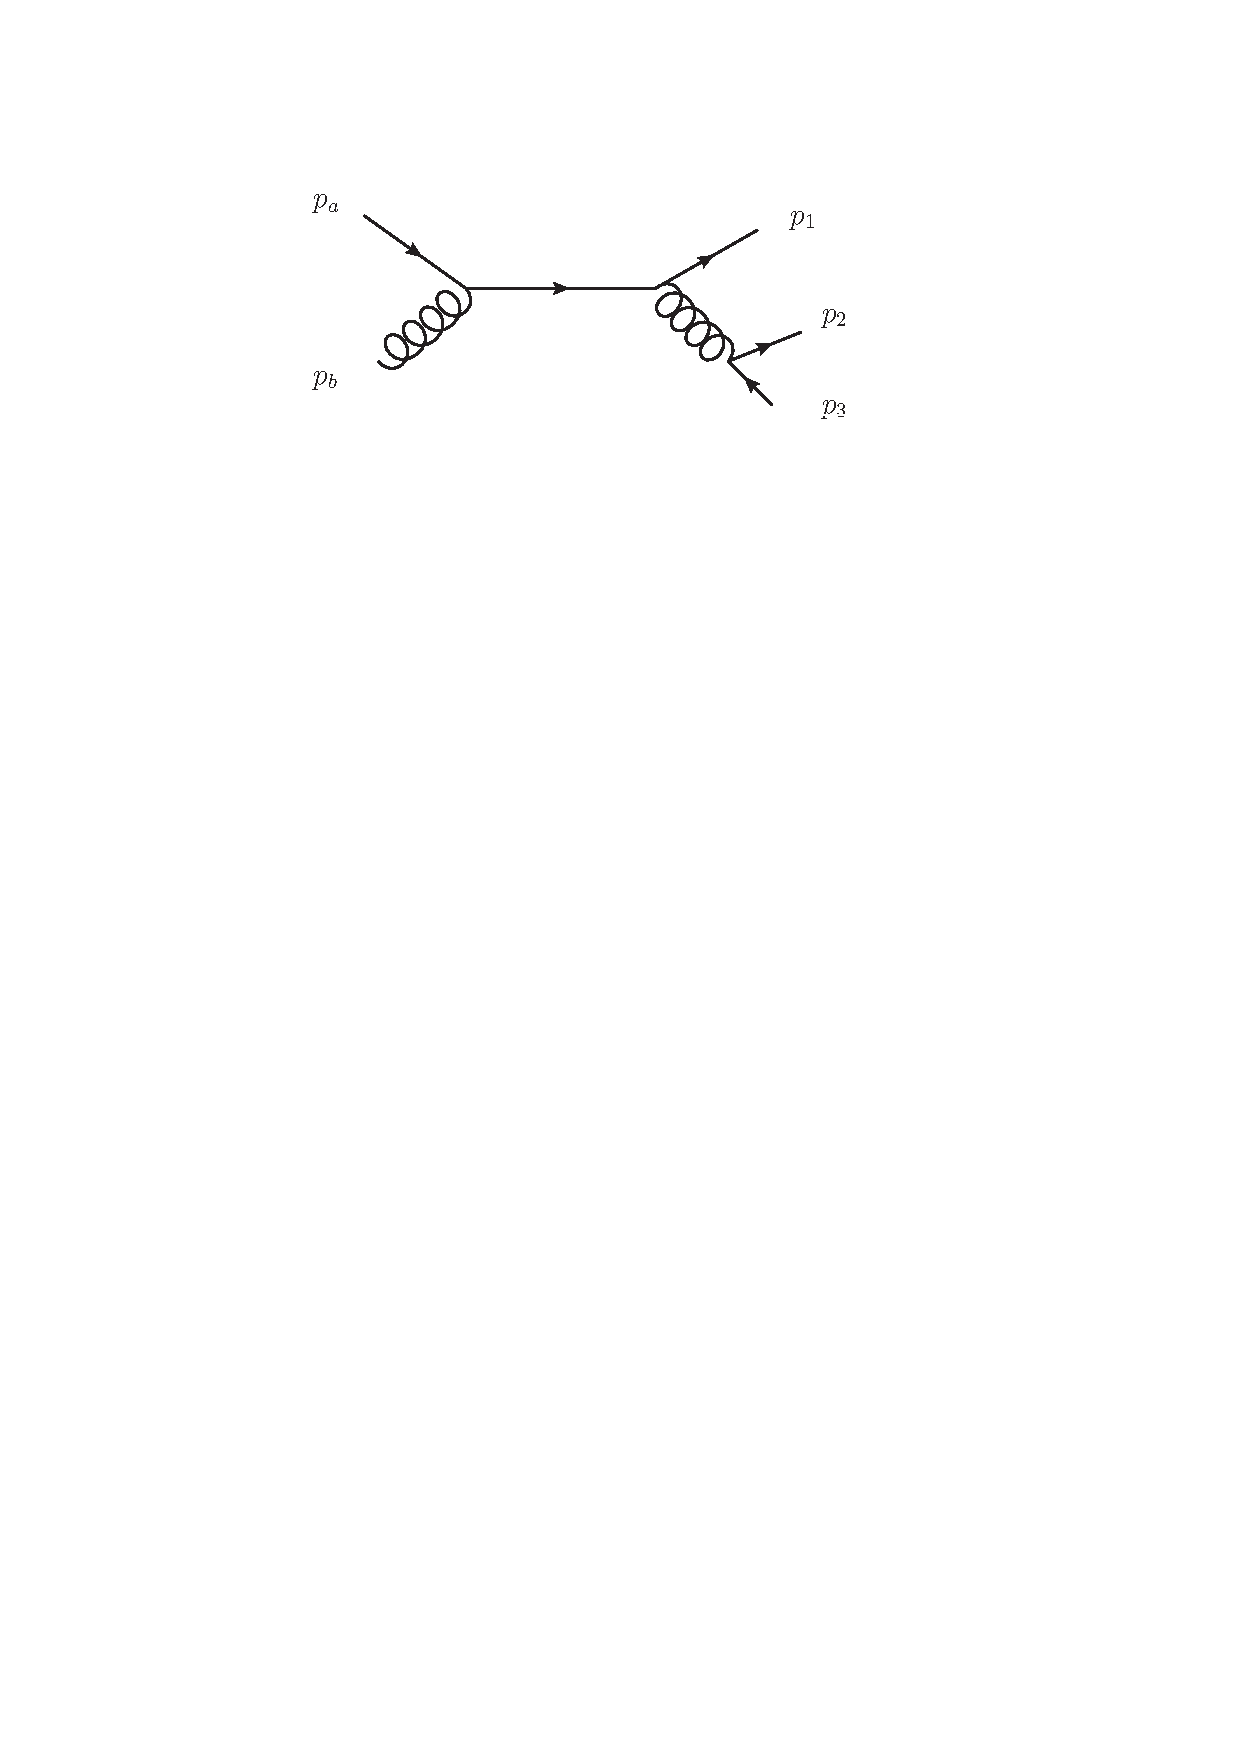
\includegraphics[scale=0.8]{Images/qg_qQQbar_s.pdf}} 
\subfloat{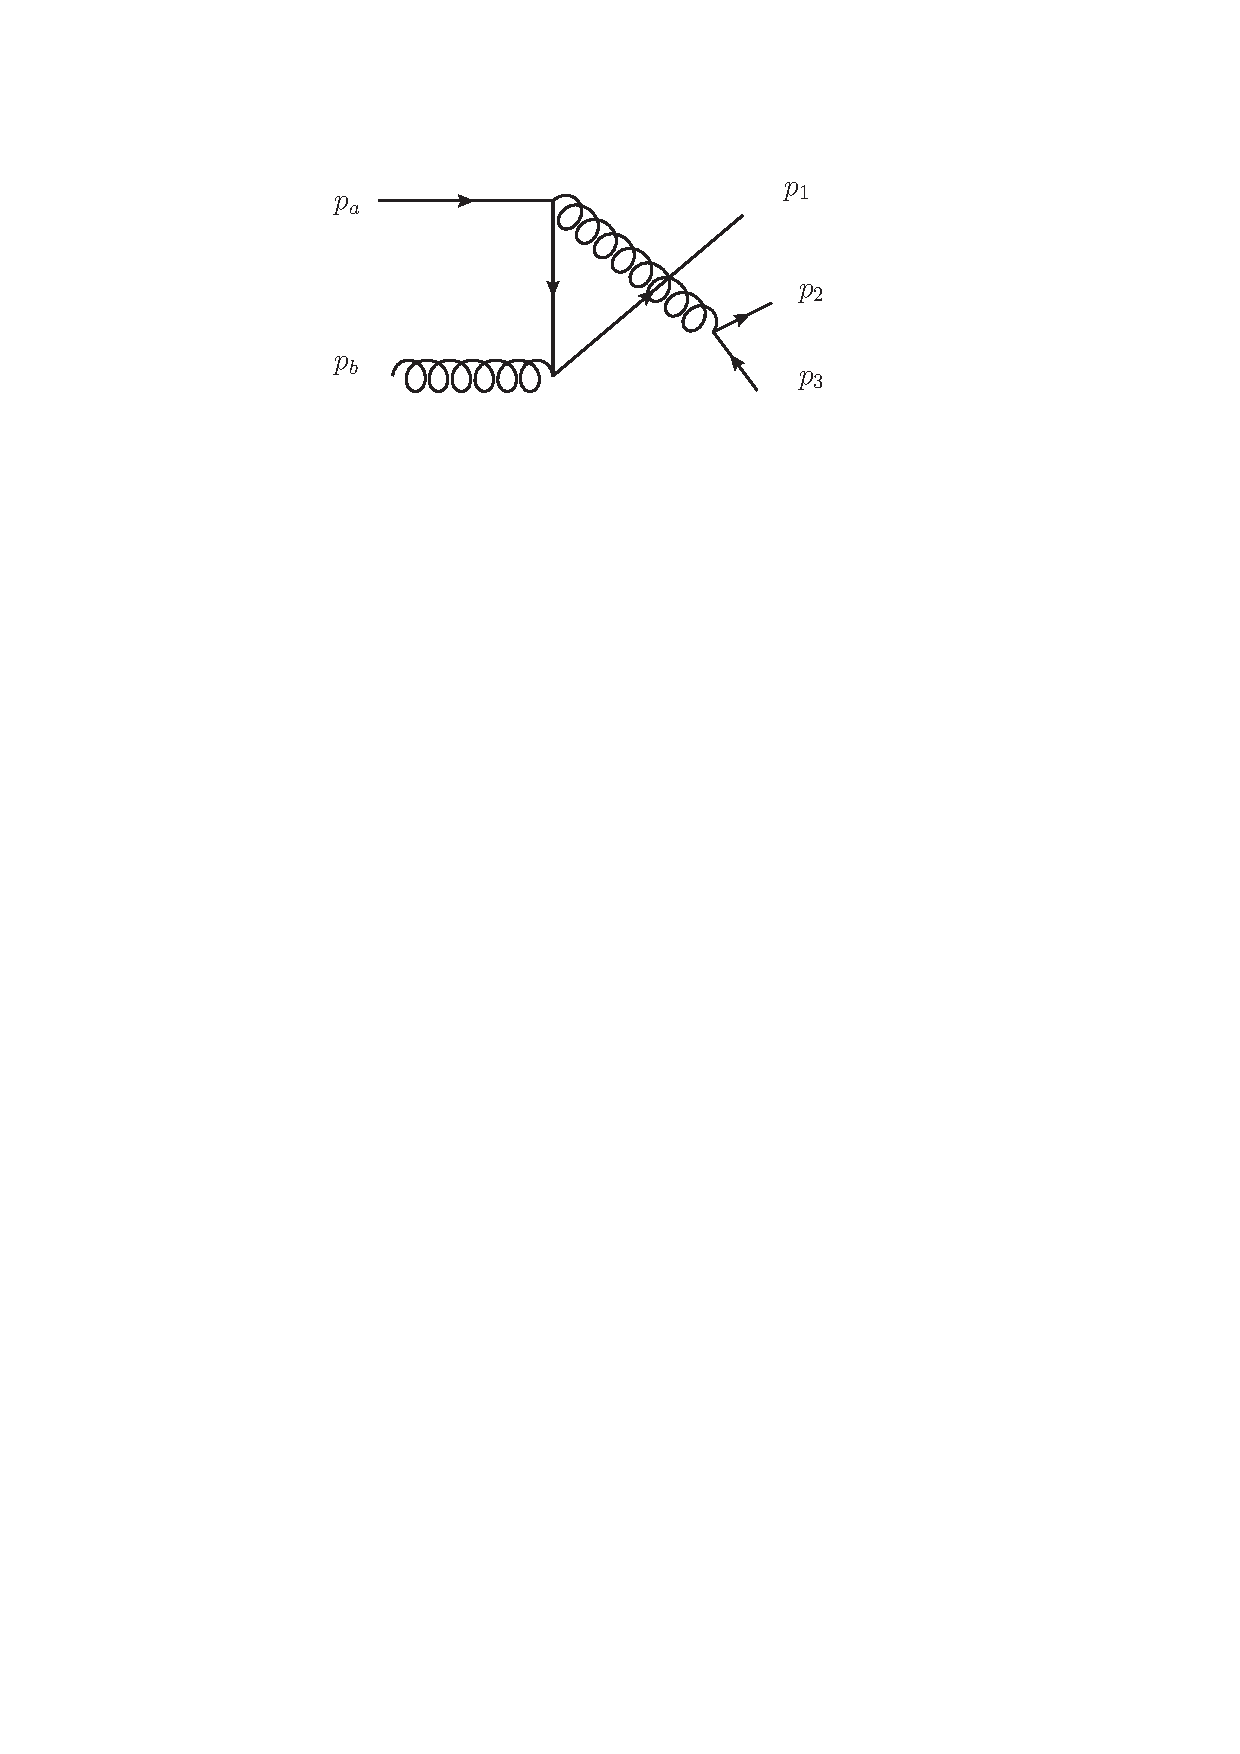
\includegraphics[scale=0.8]{Images/qg_qQQbar_u.pdf}} \\
\subfloat{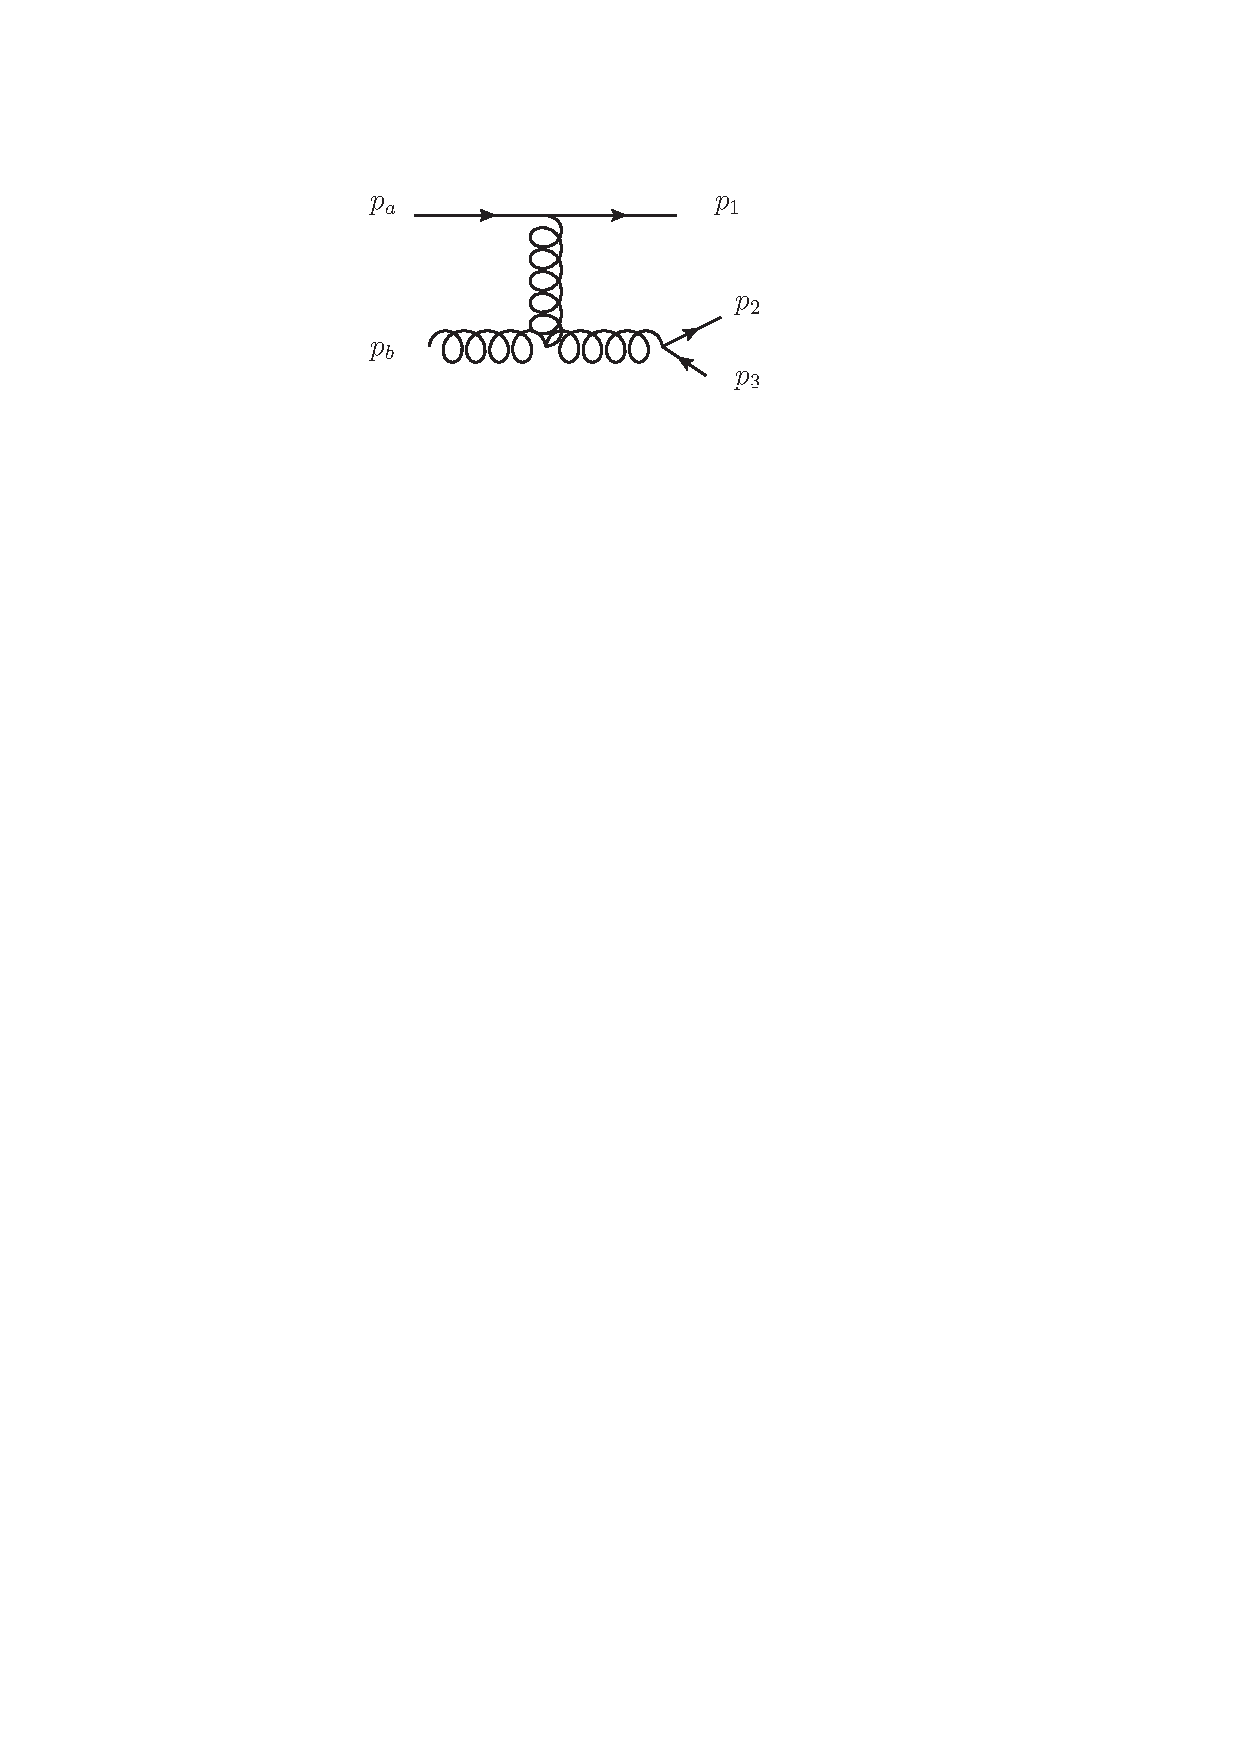
\includegraphics[scale=1]{Images/qg_qQQbar_t.pdf}} 
\subfloat{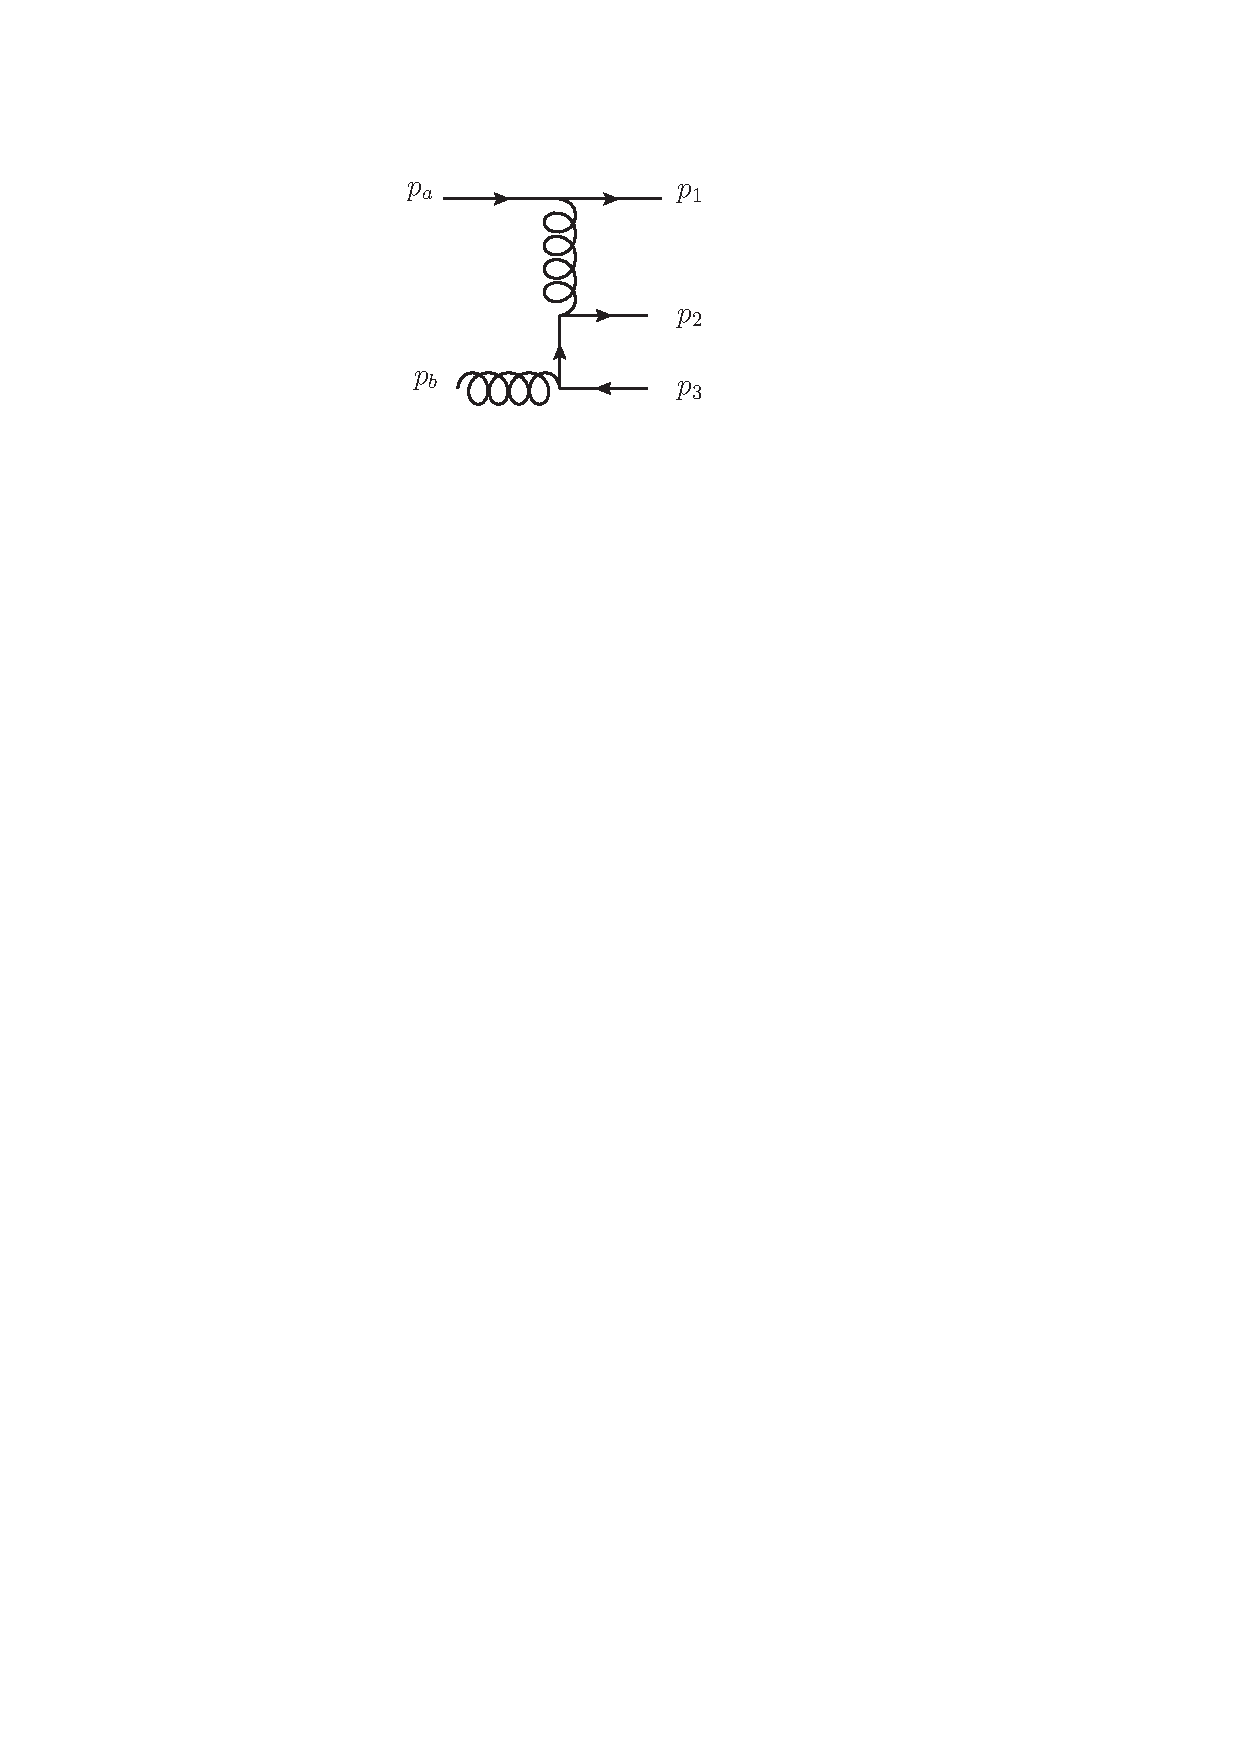
\includegraphics[scale=1]{Images/qg_qQQbar_cross.pdf}} \\
\subfloat{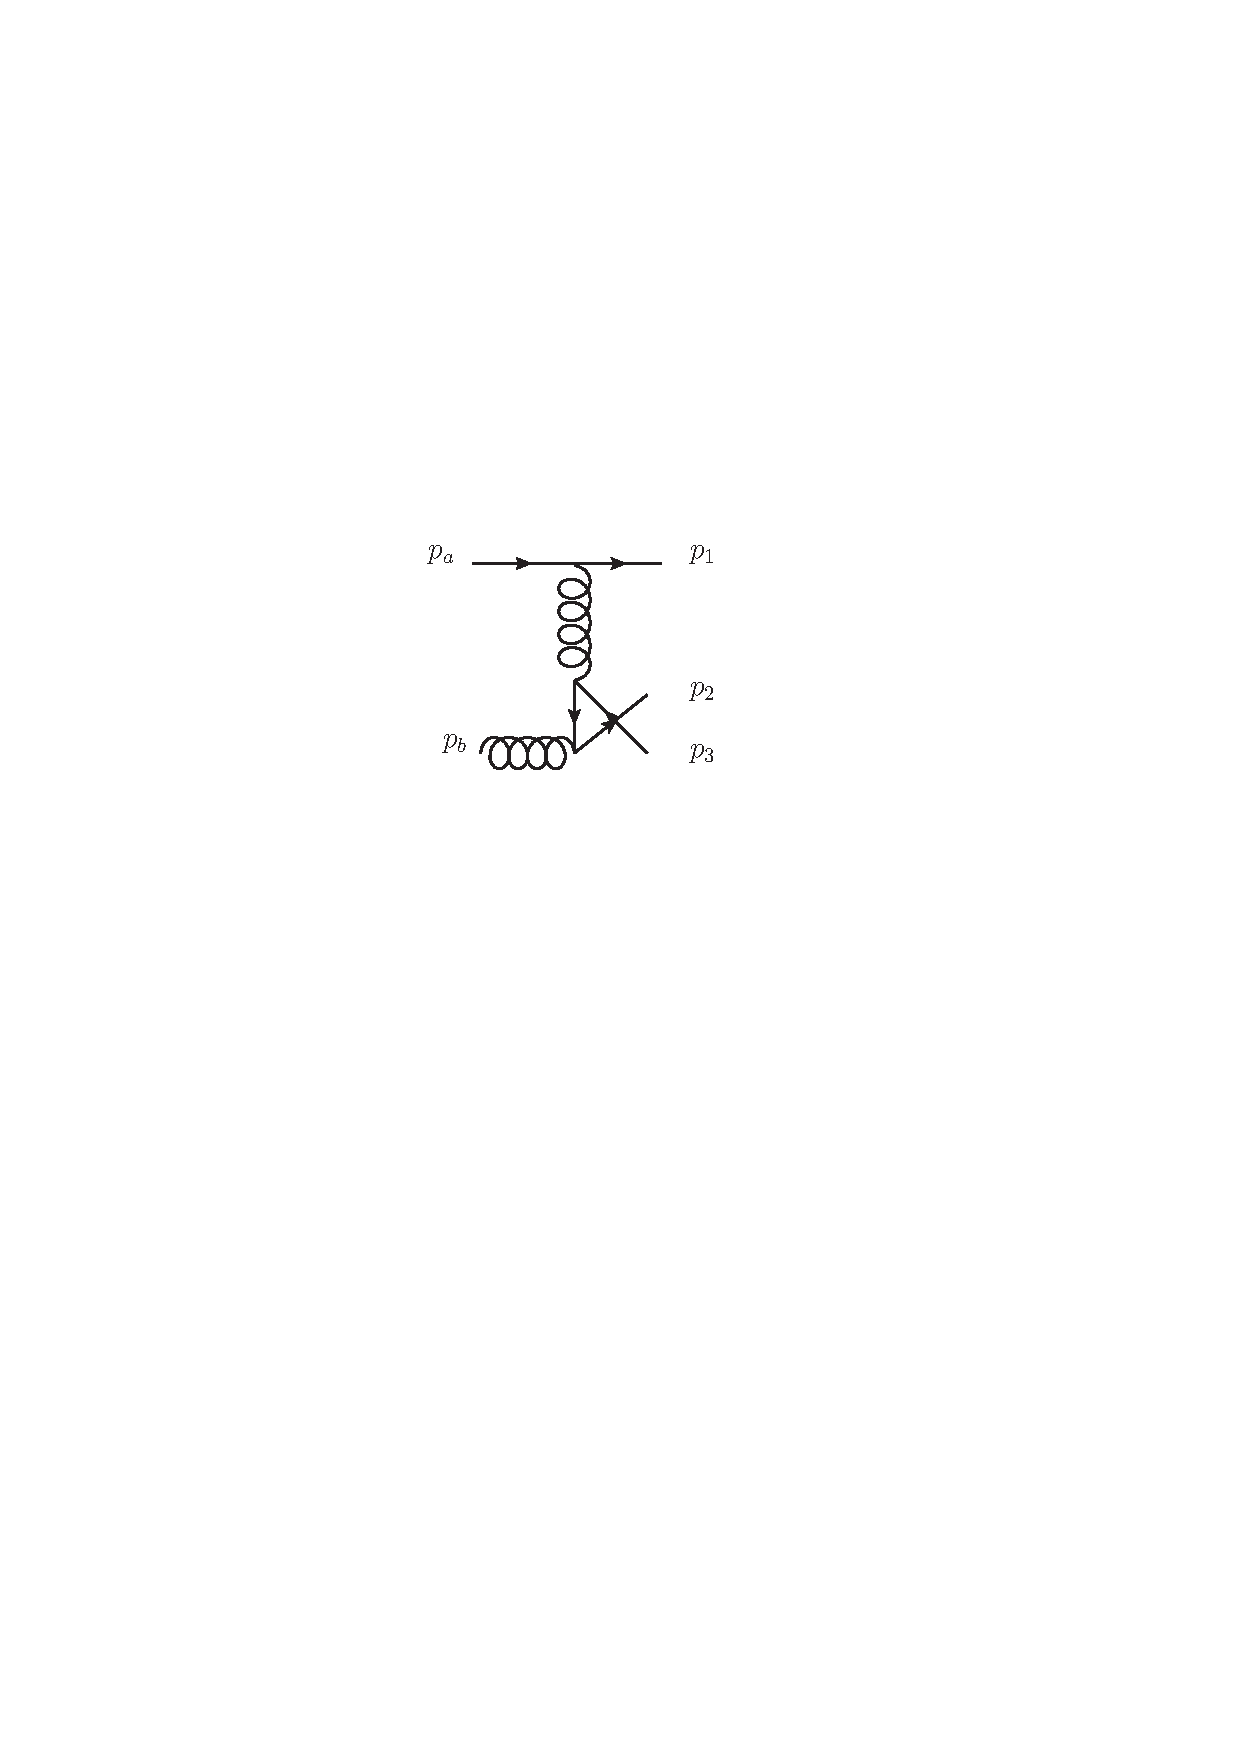
\includegraphics[scale=1]{Images/qg_qQQbar_cross2.pdf}}
\caption{All LO graphs for $qg \to qQ\bar{Q}$.}
\label{fig:qg_qQQ_graphs}
\end{figure}


The technique for this is as follows. We will first study the complete amplitude for $qg \to qQ\bar{Q}$, for which there are five contributing diagrams as shown in figure \ref{fig:qg_qQQ_graphs}. After we have the full LO expression, we will make some approximations based on the High Energy behaviour of the process to bring the entire amplitude into the desired form. During this approximation stage, we must remember to take care to maintain gauge invariance. 

We will begin with the diagram shown in the top left and then proceed from left to right and top to bottom. Using the Feynman rules, we see this contribution is;

\begin{equation}
\begin{split}
iM_1 &= \bar{u}_1(-ig_s\gamma^\nu T^g_{1q})\frac{i(\slashed{p}_a+\slashed{p}_b)}{s_{ab}}(-ig_s \gamma^\mu T_{qa}^b)u_a \varepsilon_\mu(p_b) \frac{-i \eta^{\nu \sigma}}{s_{23}} \matel{2}{\sigma}{3} (- i g_s T^g_{23}) \\
&= \frac{i g_s^3 T^g_{1q}T^b_{qa}T^g_{23}}{s_{ab}s_{23}} \left[ \bar{u}_1 \gamma^\nu (\slashed{p}_a + \slashed{p}_b) \gamma^\mu u_a \right] \matel{2}{\nu}{3} \varepsilon_\mu (p_b).
\end{split}
\end{equation}

For the diagram involving a $u$-channel quark propagator, the expression is very similar;

\begin{equation}
iM_2 = \frac{-i g_s^3 T^b_{1q}T^g_{qa}T^g_{23}}{s_{1b}s_{23}} \left[ \bar{u}_1 \gamma^\mu (\slashed{p}_1 - \slashed{p}_b) \gamma^\nu u_a \right] \matel{2}{\nu}{3} \varepsilon_\mu (p_b).
\end{equation}

The next diagram involves a three-gluon vertex and by invoking the Feynman rules we get;

\begin{equation}
iM_3 = \left[\bar{u}_1(-i g_s \gamma^\mu T^g_{1a}) u_a \right] \frac{-i \eta_{\mu \nu}}{\hat{t}_1} \left[\bar{u}_2 (-i g_s \gamma^\rho T^{g'}_{23}) u_3 \right] \frac{- i \eta_{\beta \rho}}{s_{23}} (-g_s f^{g g' b})V_{3g}^{\nu  \beta \alpha} \varepsilon_\alpha(p_b),
\end{equation}

where;

\begin{equation}
V_{3g}^{\nu \beta \alpha} = (p_a - p_1 +p_2 + p_3)^\alpha \eta^{\nu \beta} - (p_2 + p_3 + p_b)^\nu \eta^{\beta \alpha} + (p_b -p_a + p_1)^\beta \eta^{ \alpha \nu}. 
\end{equation}

Algebraic manipulation of this expression leads to;

\begin{equation}
iM_3 = \frac{-g_s^3 T^g_{1a} T^{g'}_{23} f^{g g' b}}{t_1 s_{23}}  \matel{1}{\nu}{a} \matel{2}{\beta}{3} V_{3g}^{\nu \beta \alpha}\epsilon_\alpha(p_b).
\end{equation}

Finally, we have the last two diagrams that involve both a $t$-channel gluon and quark propagator. For the first, we have:

\begin{equation}
iM_4 = \left[\bar{u}_1 (-i g_s \gamma^\mu T^g_{1a}) u_a \right] \frac{-i \eta_{\mu \nu}}{\hat{t}_1} \left[\bar{u}_2 (-i g_s \gamma^\nu T^g_{2q}) \frac{-i (\slashed{p}_3 - \slashed{p}_b )}{\hat{t}_2} (-i g_s \gamma^\rho T^b_{q3})u_3 \right] \varepsilon_\rho (p_b).
\end{equation}

Note the minus sign in the propagator; this is because the Feynman rule for the quark propagator requires that the momentum flows in the same direction as the charge. This can be written:

\begin{equation}
iM_4 = \frac{-i g_s^3 T^g_{1a}T^b_{q3}T^g_{2q}}{\hat{t}_1 \hat{t}_2} \matel{1}{\nu}{a}\left[\bar{u}_2 \gamma^\nu (\slashed{p}_3 - \slashed{p}_b) \gamma^\rho u_3 \right] \varepsilon_\rho (p_b).
\end{equation}

A similar analysis yields for the last diagram (no minus sign from the fermion propagator this time);

\begin{equation}
iM_5 = \frac{i g_s^3 T^g_{1a}T^b_{2q}T^g_{q3}}{\hat{t}_1 \tilde{t}_2} \matel{1}{\nu}{a}\left[\bar{u}_2 \gamma^\rho (\slashed{p}_2 - \slashed{p}_b) \gamma^\nu u_3 \right] \varepsilon_\rho (p_b),
\end{equation}

with $\tilde{t}_2 = (p_2 - p_b)^2$. We now have expressions that, when summed, will give the exact, LO result for the process $qg \to qQ\bar{Q}$. Now we must approximate in order to factorise the $t$-channel pole. No approximation is required for $M_3, M_4$ or $M_5$ since the $t$-channel pole is immediately explicit. $M_1$ and $M_2$, however, need special attention. The problematic part is the square brackets of, for example, $M_1$ which we can rewrite using the completeness relation;

\begin{equation}
\bar{u}_1 \gamma^\nu (\slashed{p}_a + \slashed{p}_b) \gamma^\mu u_a = \matel{1}{\nu}{a}2 p_a^\mu + \matel{1}{\nu}{b} \matel{b}{\mu}{a},
\end{equation}

where the spinor brackets have no helicity index written to indicate that the expansion is valid for both negative and positive helicities. The $\nu$ index is contracted with the quark current $\matel{2}{\nu}{b}$. Depending on the helicity choices, the second term after contraction behaves either like $\sqrt{s_{b3} s_{12}}$ or $\sqrt{s_{13} s_{b2}}$. Similarly, the first term behaves either like $\sqrt{s_{a3} s_{12}}$ or $\sqrt{s_{13} s_{a2}}$. The relative size of these terms is then $\sqrt{s_{b3}/s_{a3}}$ or $\sqrt{s_{b2}/s_{a2}}$. In the High Energy limit, it is clear that both $s_{a3}$ and $s_{a2}$ both are large. Also, since we are dealing with the case where the $q\bar{q}$ pair is emitted close in rapidity to one end of the chain, we can reasonably assume that $s_{b3}$ and $s_{b2}$ do not have to be large. We can therefore drop the second term with respect to the first and thus;

\begin{equation}
iM_1 \approx \frac{i g_s^3 T^g_{1q}T^b_{qa}T^g_{23}}{s_{ab}s_{23}} \left[ 2p_a^\mu \matel{1}{\nu}{a} \right] \matel{2}{\nu}{3} \varepsilon_\mu (p_b).
\end{equation}

A similar arguement holds for $M_2$ and so;

\begin{equation}
iM_2 \approx \frac{-i g_s^3 T^b_{1q}T^g_{qa}T^g_{23}}{s_{1b}s_{23}} \left[ 2p_1^\mu \matel{1}{\nu}{a} \right] \matel{2}{\nu}{3} \varepsilon_\mu (p_b).
\end{equation}

We can now take the limit that $p_a \sim p_1$, which allows us to combine these two diagrams by using the colour commutator result:

\begin{equation}
(T^g_{1q}T^b_{qa}- T^b_{1q}T^g_{qa})T^g_{23} = i f^{gbc}T^c_{1a}T^g_{23}.
\end{equation}

This is the same colour factor as that of the diagram involving a $t$-channel gluon exchange under the relabelling $g \to c$ and $g' \to g$. Because of this, we will from now on call the result of this $i C_t$. Thus;

\begin{equation}
i(M_1 + M_2) \to \frac{- g_s^3 C_t}{s_{ab}s_{23}}2p_a^\mu \matel{1}{\nu}{a} \matel{2}{\nu}{3} \varepsilon_\mu (p_b),
\end{equation}

and so we have now factored out the quark current in all the amplitudes. If we now combine all the amplitudes together, then we get the form of $Q^{\mu \nu}$ to be:

\begin{equation}
\begin{split}
Q^{\mu \nu} &= -\frac{C_1}{\hat{t}_2} \left(\bar{u}_2 \gamma^\mu (\slashed{p}_3-\slashed{p}_b)\gamma^\nu u_3 \right) + \frac{C_2}{\tilde{t}_2} \left( \bar{u}_2 \gamma^\nu (\slashed{p}_2-\slashed{p}_b) \gamma^\mu u_3 \right) \\
&+ i  \frac{C_t}{s_{23}} \left(\frac{2 \hspace{2pt} p_a^\nu \hspace{2pt} \hat{t}_1}{s_{ab}}  \matel{2}{\mu}{3} + V^{\mu \rho \nu}_{3g}  \matel{2}{\rho}{3} \right),
\end{split}
\end{equation}

where we have relabelled some Lorentz indices to conform with equation \ref{eqn:NLLeqn} and where;

\begin{subequations}
\begin{align}
C_1 &= T^g_{1a} T^b_{q3}T^g_{2q}, \\
C_2 &= T^g_{1a} T^b_{2q}T^g_{q3}, \\
C_t &= f^{gbc}T^c_{1a}T^g_{23}.
\end{align}
\end{subequations}

We should check at this point that our expression is indeed still gauge invariant after having made these approximations. The simplest way to check is to make use of the Ward Identity, which implies $Q^{\mu \nu} p_{b, \nu} = 0$. Explicitly; 

\begin{equation}
\begin{split}
Q^{\mu \nu}p_{b, \nu} &= -\frac{C_1}{\hat{t}_2} \left(\bar{u}_2 \gamma^\mu \slashed{p}_3 \slashed{p_b} u_3 \right) + \frac{C_2}{\tilde{t}_2} \left( \bar{u}_2 \slashed{p}_b \slashed{p}_2 \gamma^\mu u_3 \right) + i  \frac{C_t}{s_{23}} \left(\hat{t}_1  \matel{2}{\mu}{3} + V^{\mu \rho \nu}_{3g}p_{b \nu}  \matel{2}{\rho}{3} \right) \\
&= -\frac{C_1}{\hat{t}_2} s_{3b} \matel{2}{\mu}{3} + \frac{C_2}{\tilde{t}_2} s_{2b} \matel{2}{\mu}{3} + i \frac{C_t}{s_{23}}(\hat{t}_1 \matel{2}{\mu}{3} + (s_{2b} + s_{3b})\matel{2}{\mu}{3} - \\
&(p_2+p_3+p_b)^\mu p_b^\rho\matel{2}{\rho}{3} + 2p_b^\mu p_b^\rho \matel{2}{\rho}{3}) \\
&= \frac{\matel{2}{\mu}{3}}{s_{23}}(C_1 s_{23} - C_2 s_{23} + i C_t(\hat{t}_1 + (s_{2b} + s_{3b})) \\
&+ i\matel{2}{\rho}{3} \frac{C_t}{s_{23}}(-(p_2+p_3+p_b)^\mu p_b^\rho + 2p_b^\mu p_b^\rho) \\
&= i C_t \frac{\matel{2}{\mu}{3}}{s_{23}}(-s_{23} + (-s_{2b} - s_{3b} + s_{23} + s_{2b} + s_{3b})) \\
&+i\matel{2}{\rho}{3} \frac{C_t}{s_{23}}(-(p_2+p_3+p_b)^\mu p_b^\rho + 2p_b^\mu p_b^\rho)) \\
&\approx  i C_t \frac{\matel{2}{\rho}{3}}{s_{23}}(-2p_b^\mu p_b^\rho + 2p_b^\mu p_b^\rho)) \\
&= 0,
\end{split}
\end{equation}

where we have had to make the high energy approximation $p_b \sim p_2 + p_3$. Therefore, so long as we always approximate the three gluon vertex in this manner (this is where the `offending' term came from), the effective vertex is, indeed, a gauge invariant quantity. It may seem, however, that the effective vertex is not truly factorised since there is a clear instance of $p_a$ in the vertex. Because the complete term goes like $p_a^\mu/s_{ab}$, it is actually independent of $p_a$\footnote{An easy way to convince oneself of this is to work in light-cone co-ordinates and see that the $p_a^+$ scale factors out on the top and bottom of the expression.}. We still have freedom to make a gauge choice to do our calculations in, however, and a good choice will be the gauge where the gluon polarisation vector is orthogonal to $p_a$ and we have;

\begin{equation}
\begin{split}
Q^{\mu \nu}_{gauge} &= -\frac{C_1}{\hat{t}_2} \left(\bar{u}_2 \gamma^\mu (\slashed{p}_3-\slashed{p}_b)\gamma^\nu u_3 \right) + \frac{C_2}{\tilde{t}_2} \left( \bar{u}_2 \gamma^\nu (\slashed{p}_2-\slashed{p}_b) \gamma^\mu u_3 \right)  \\
&+ i  \frac{C_t}{s_{23}} \left((2p_2+2p_3)^\nu \eta^{\mu \rho} - 2p_b^\mu \eta^{\nu \rho} + 2p_b^\rho \eta^{\nu \mu} \right) \matel{2}{\rho}{3},
\end{split}
\end{equation}

completing our calculation for the basis HEJ amplitude in the case of an extremal $q \bar{q}$ process.

\subsection{Calculation of $qq' \to qQ\bar{Q}q'$ in the High Energy Limit}

The technique for calculating the amplitude for the central process is precisely the same as the one for the extremal process. In this case, we are searching for an amplitude of the form;

\begin{equation}
M_{qq' \to qQ\bar{Q}q'} \sim \frac{\matel{1}{\mu}{a}X^{\mu \nu} \matel{4}{\nu}{b}}{\hat{t}_1 \hat{t}_3}.
\end{equation}

\begin{figure}[t]
\centering
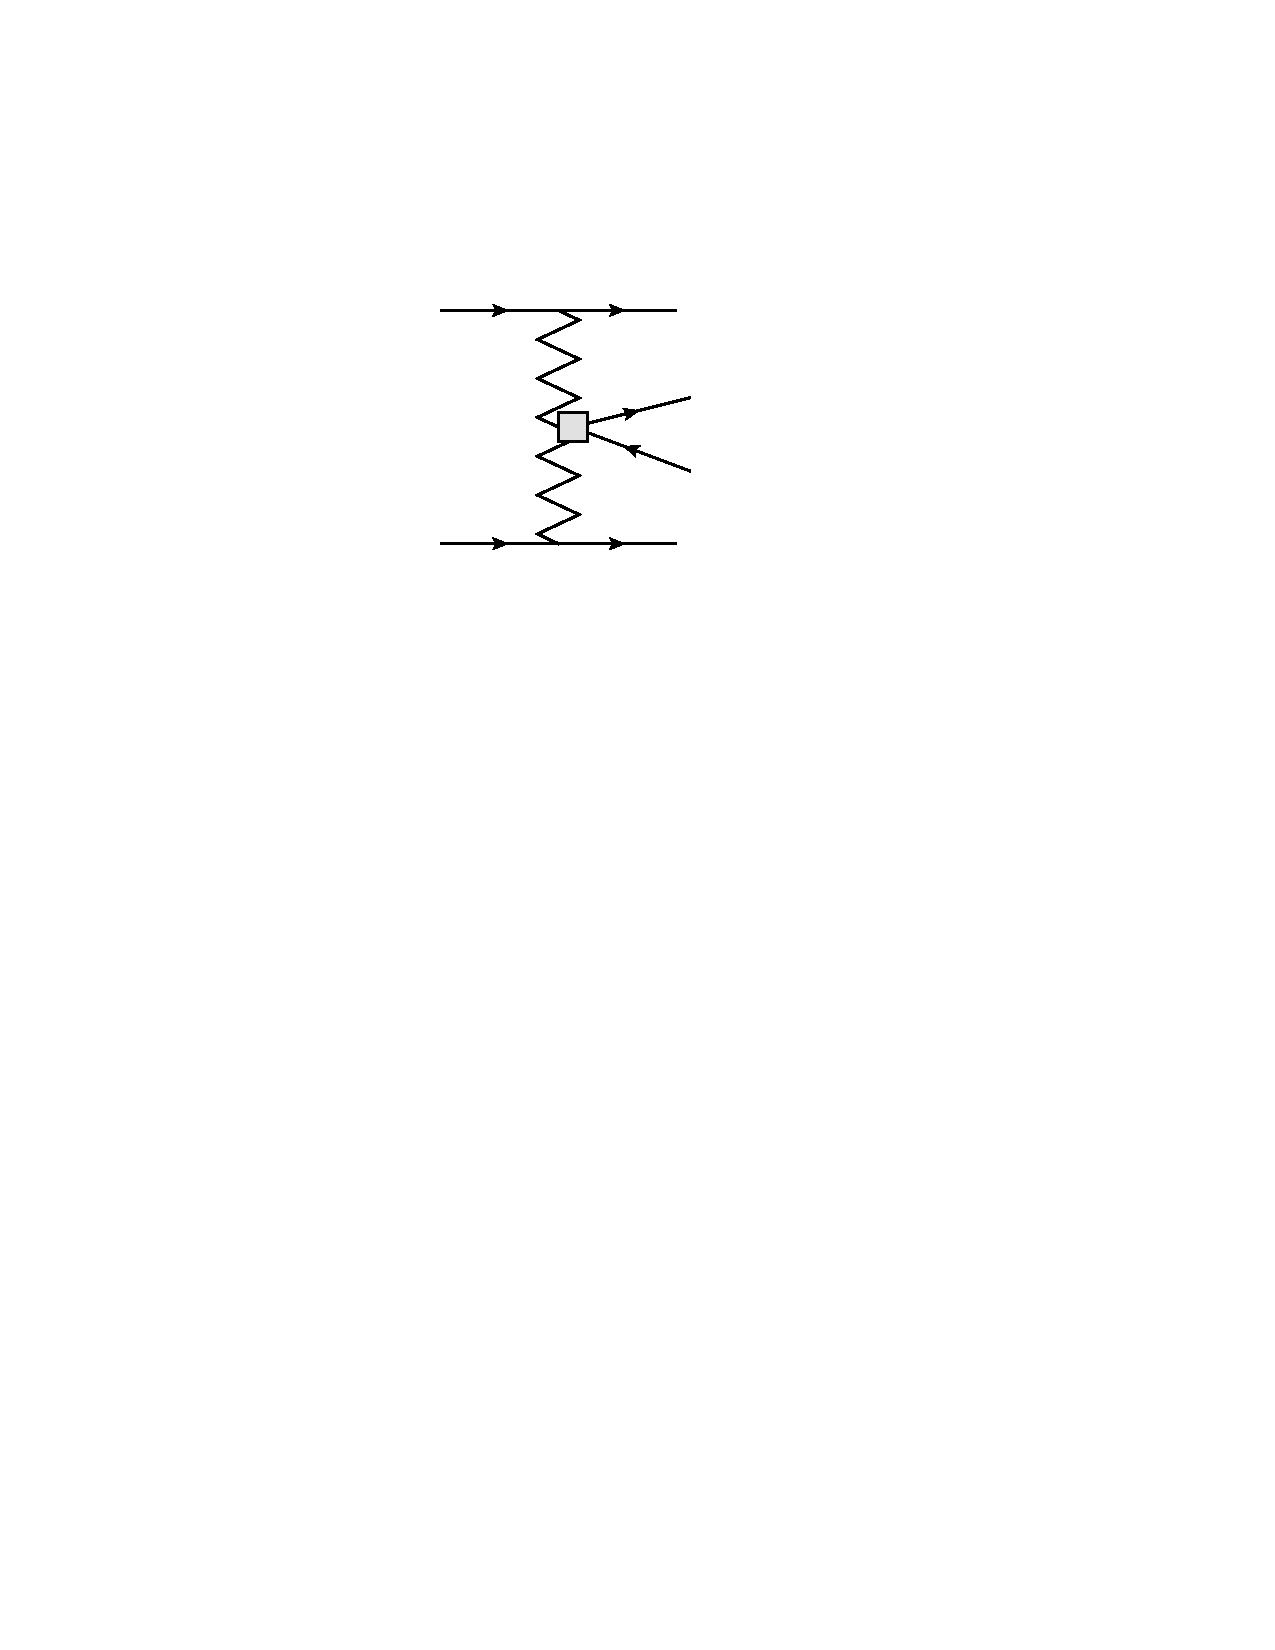
\includegraphics{Images/qq_qqqq_eff.pdf}
\caption{Effective description of $qQ \to qq'\bar{q}' Q$}
\end{figure}

There are a total of 7 diagrams to calculate here, shown in figure \ref{fig:qq_qQQq_graphs}. Once more, we will calculate the diagrams starting with the one in the top left and proceeding left to right. The expression for the first diagram is;

\begin{equation}
iM_1 = \frac{- i g_s^4 T^e_{1q}T^g_{qa}T^e_{23}T^g_{4b}}{s_{23} \hat{t}_3} \left[ \bar{u}_1 \gamma^\mu \frac{(\slashed{p}_1+\slashed{p}_2 + \slashed{p}_3)}{(p_1 + p_2 + p_3)^2} \gamma^\rho u_a \right] \left[\bar{u}_2 \gamma_\mu u_3 \right] \left[ \bar{u}_4 \gamma_\rho u_b \right].
\end{equation}

\begin{figure}[H] 
\centering
\subfloat{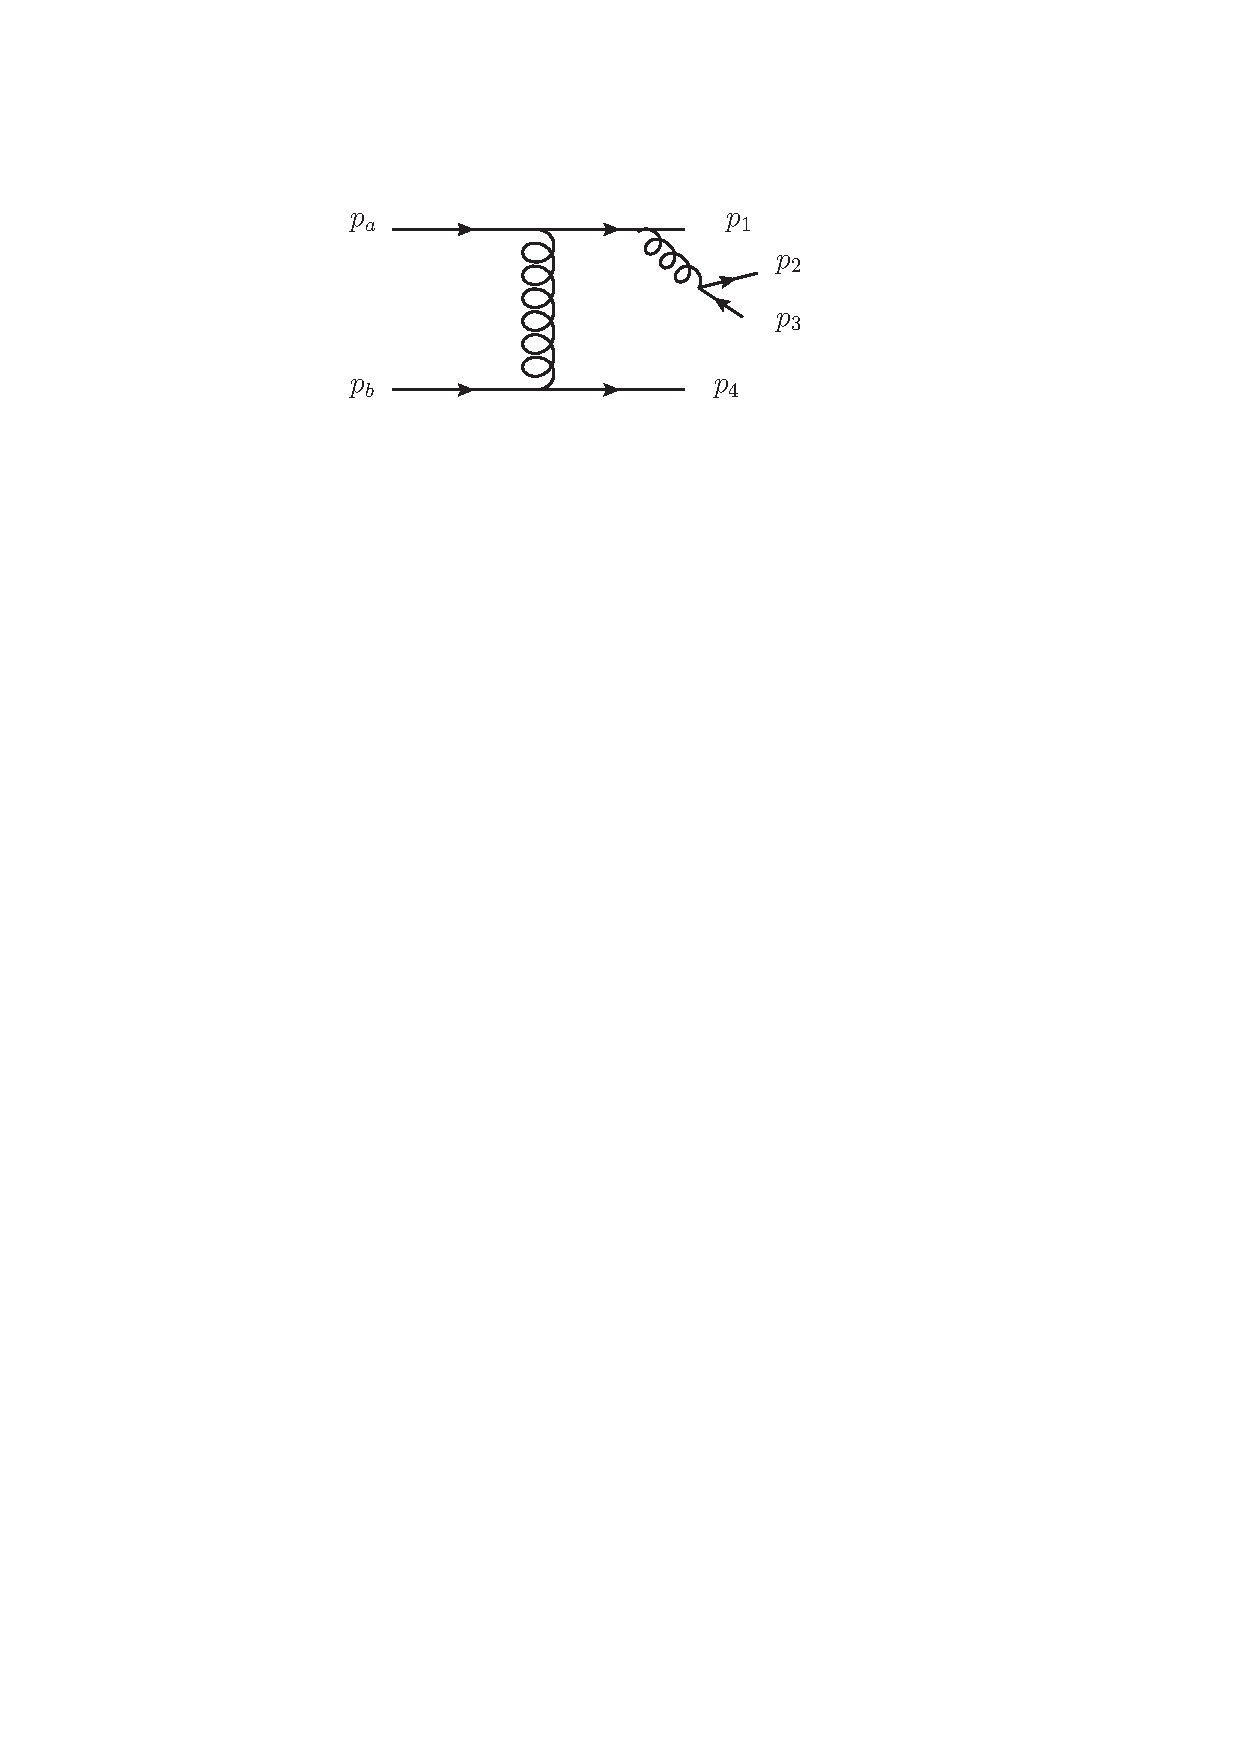
\includegraphics[scale=0.65]{Images/4j_p1_emission.pdf}} 
\subfloat{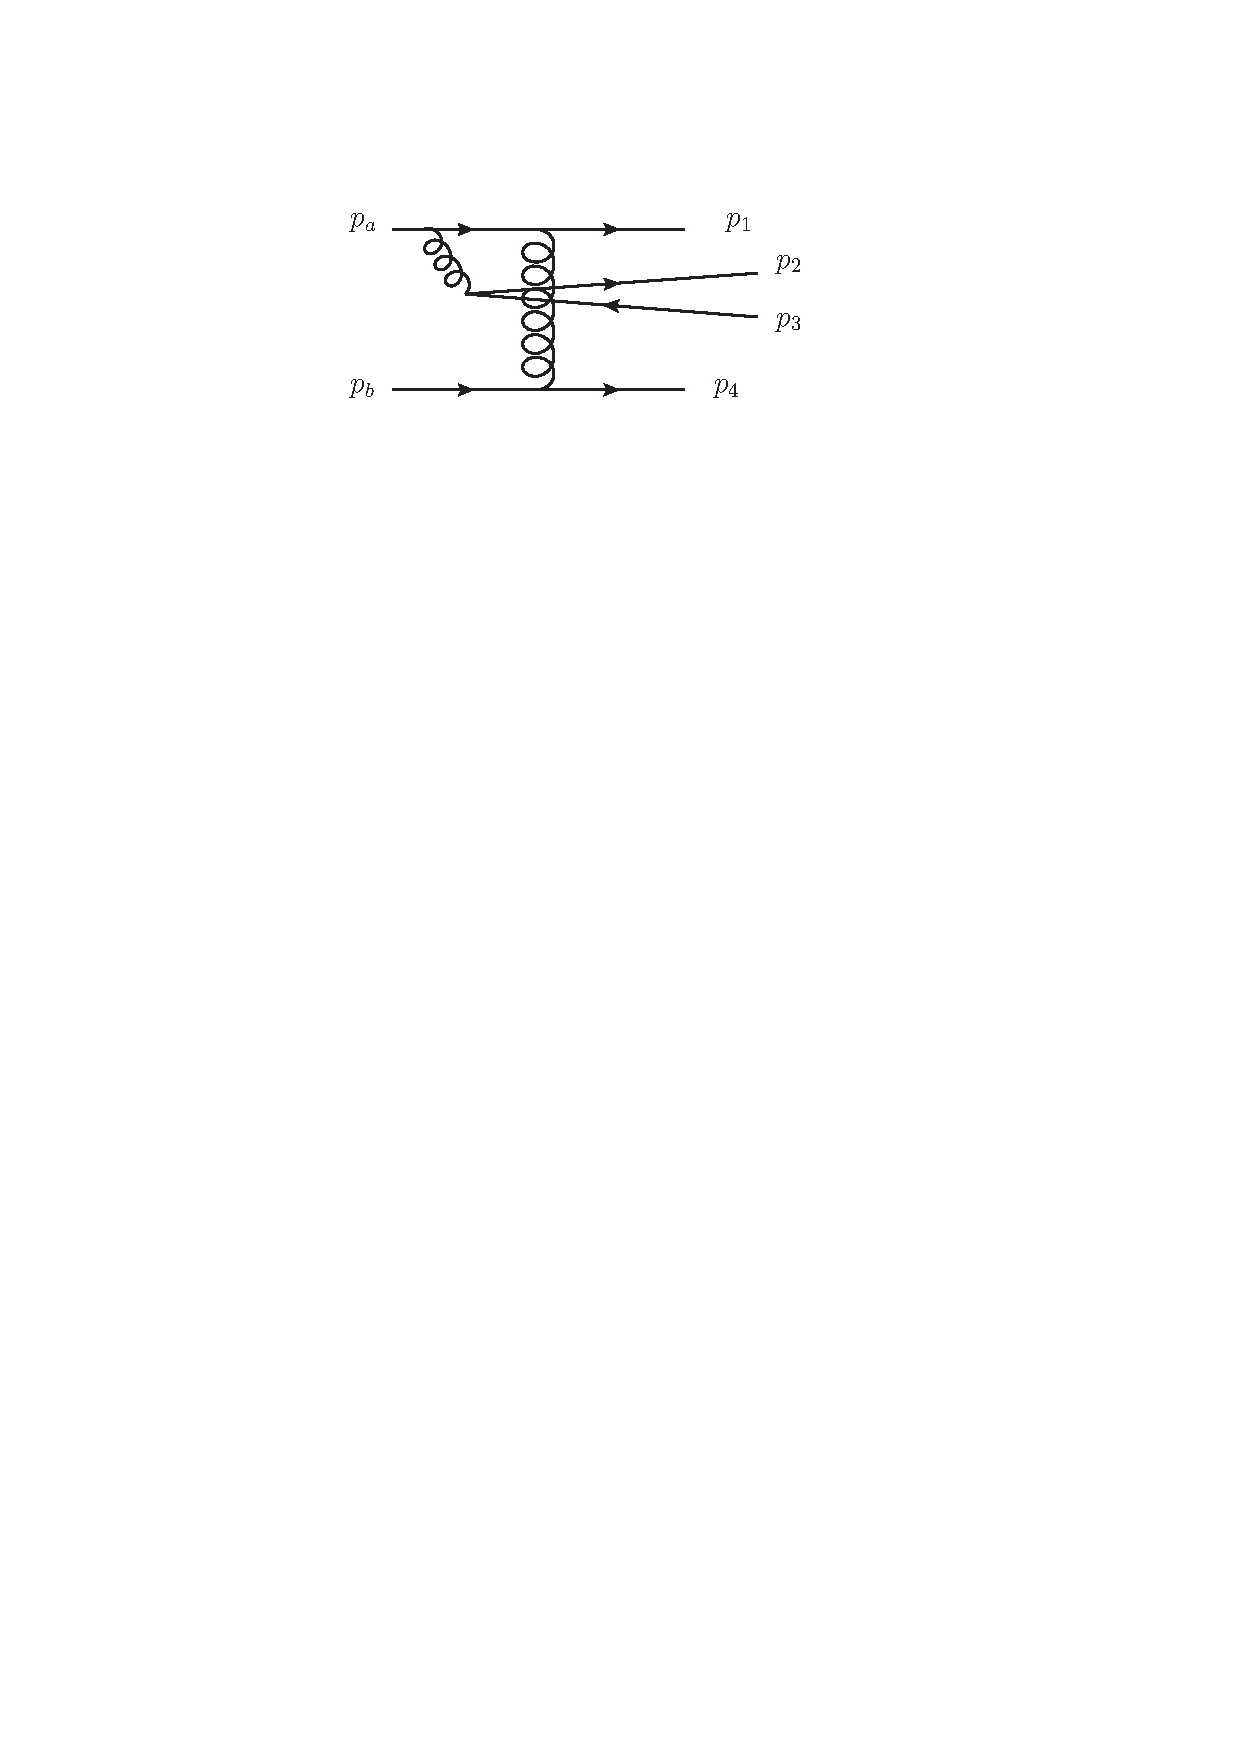
\includegraphics[scale=0.65]{Images/4j_pa_emission.pdf}} 
\subfloat{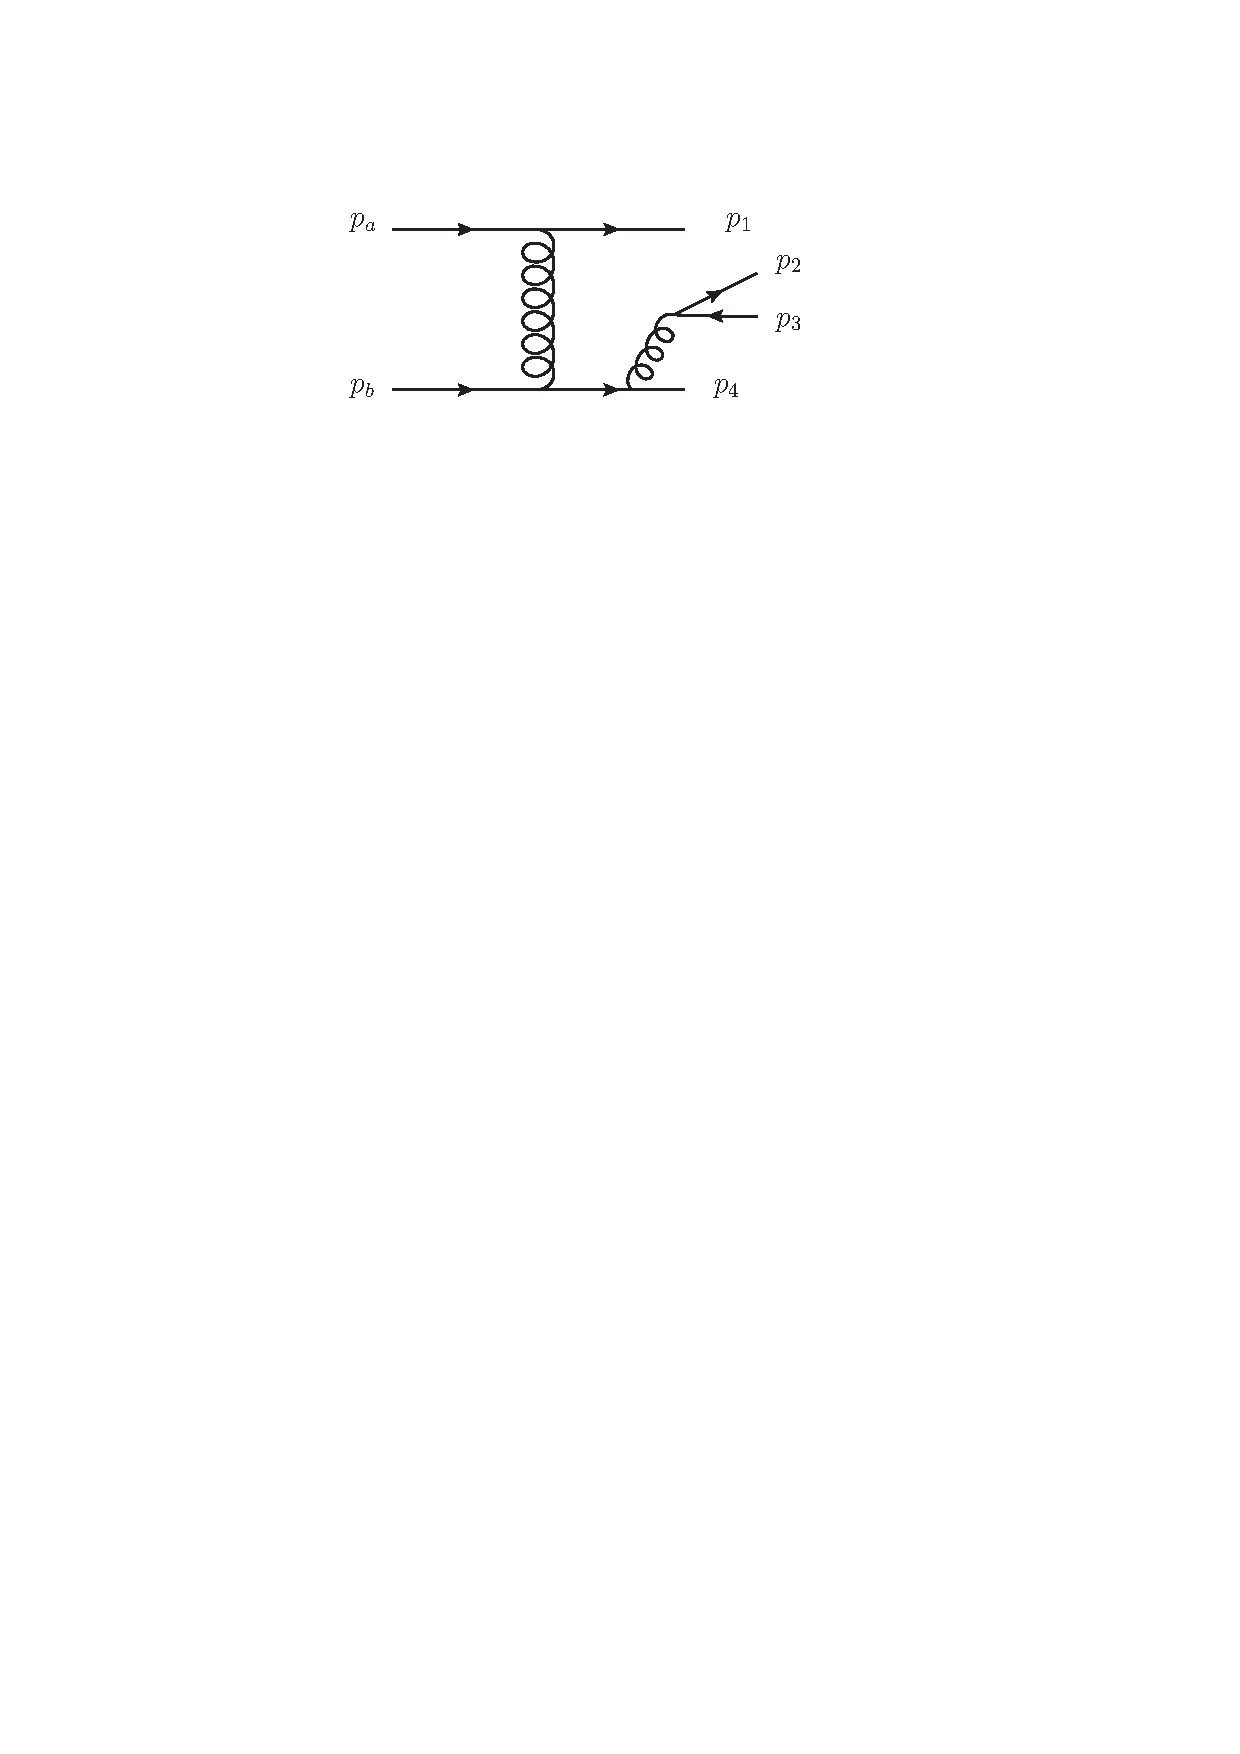
\includegraphics[scale=0.65]{Images/4j_p4_emission.pdf}} \\
\subfloat{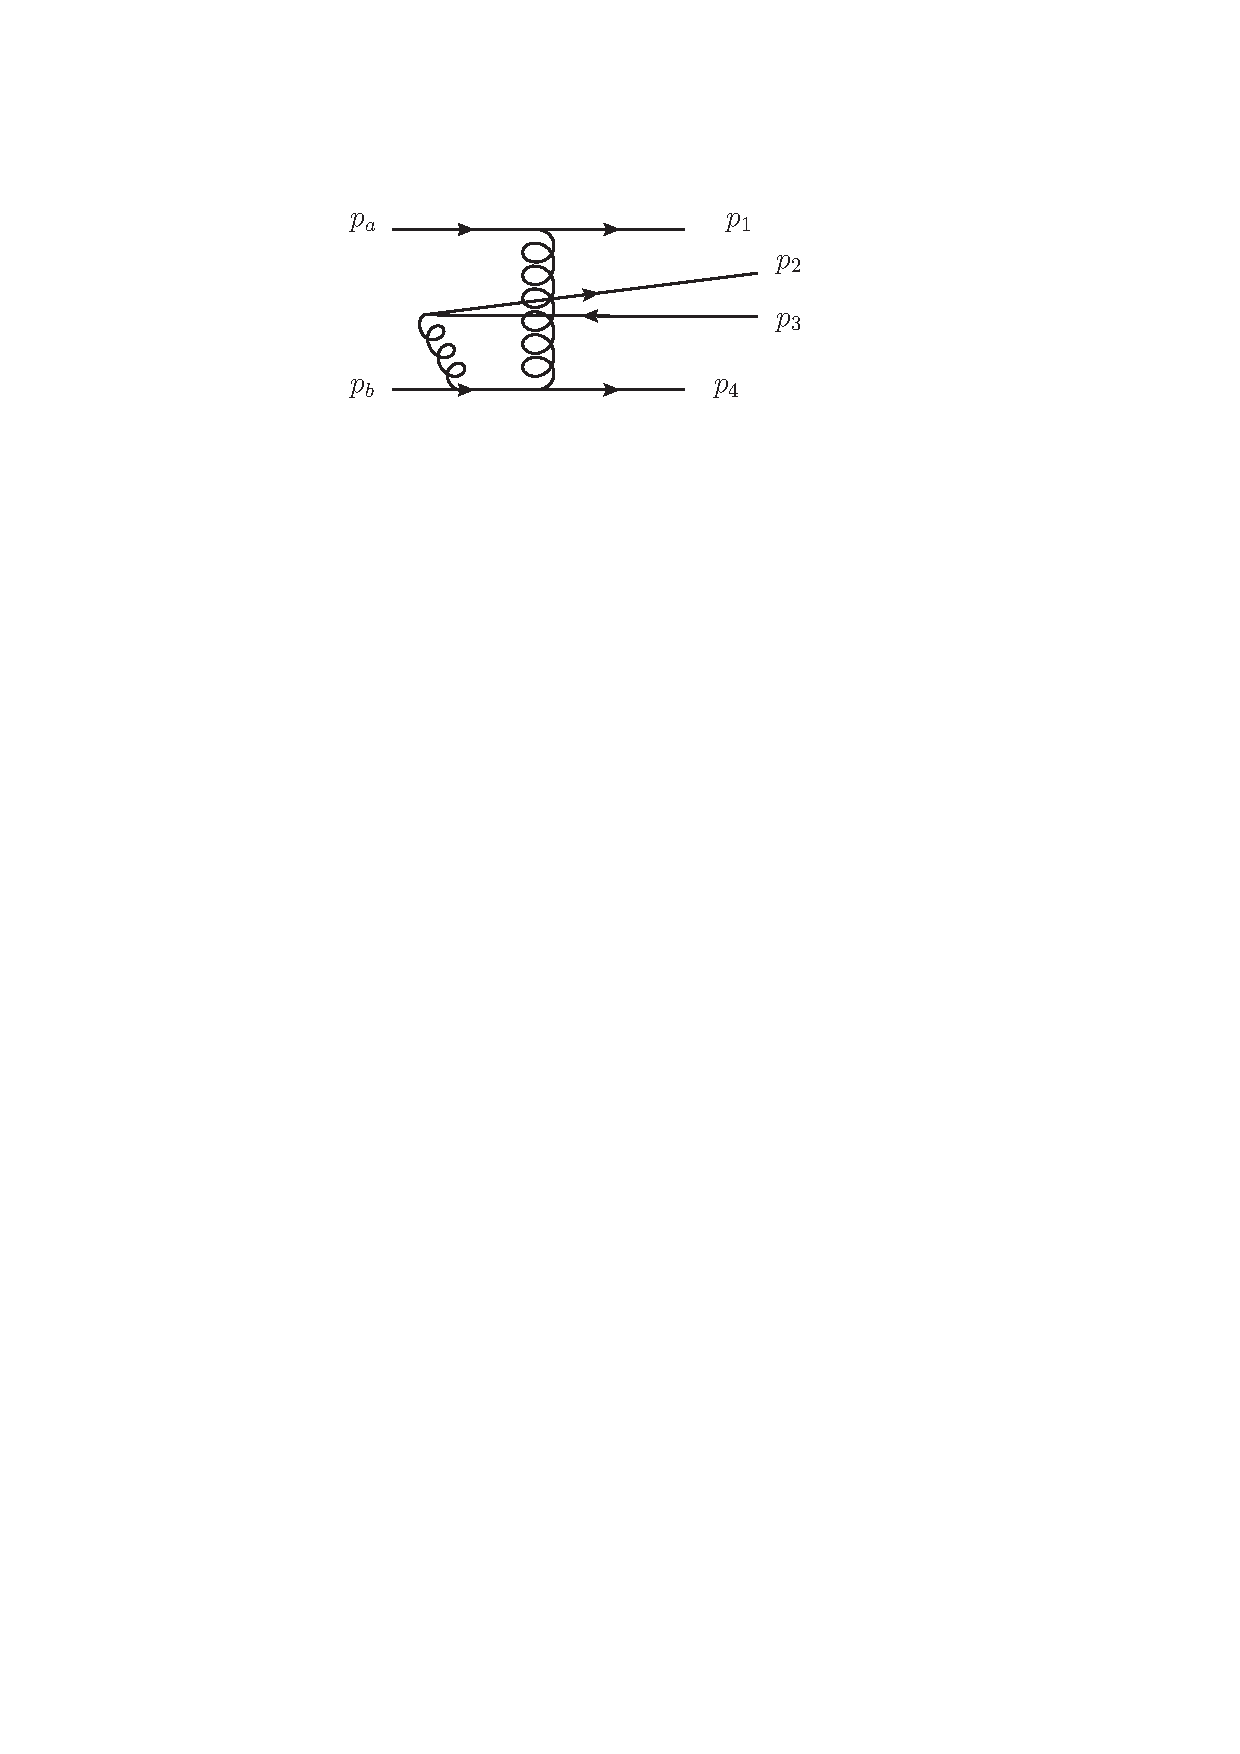
\includegraphics[scale=0.65]{Images/4j_pb_emission.pdf}} 
\subfloat{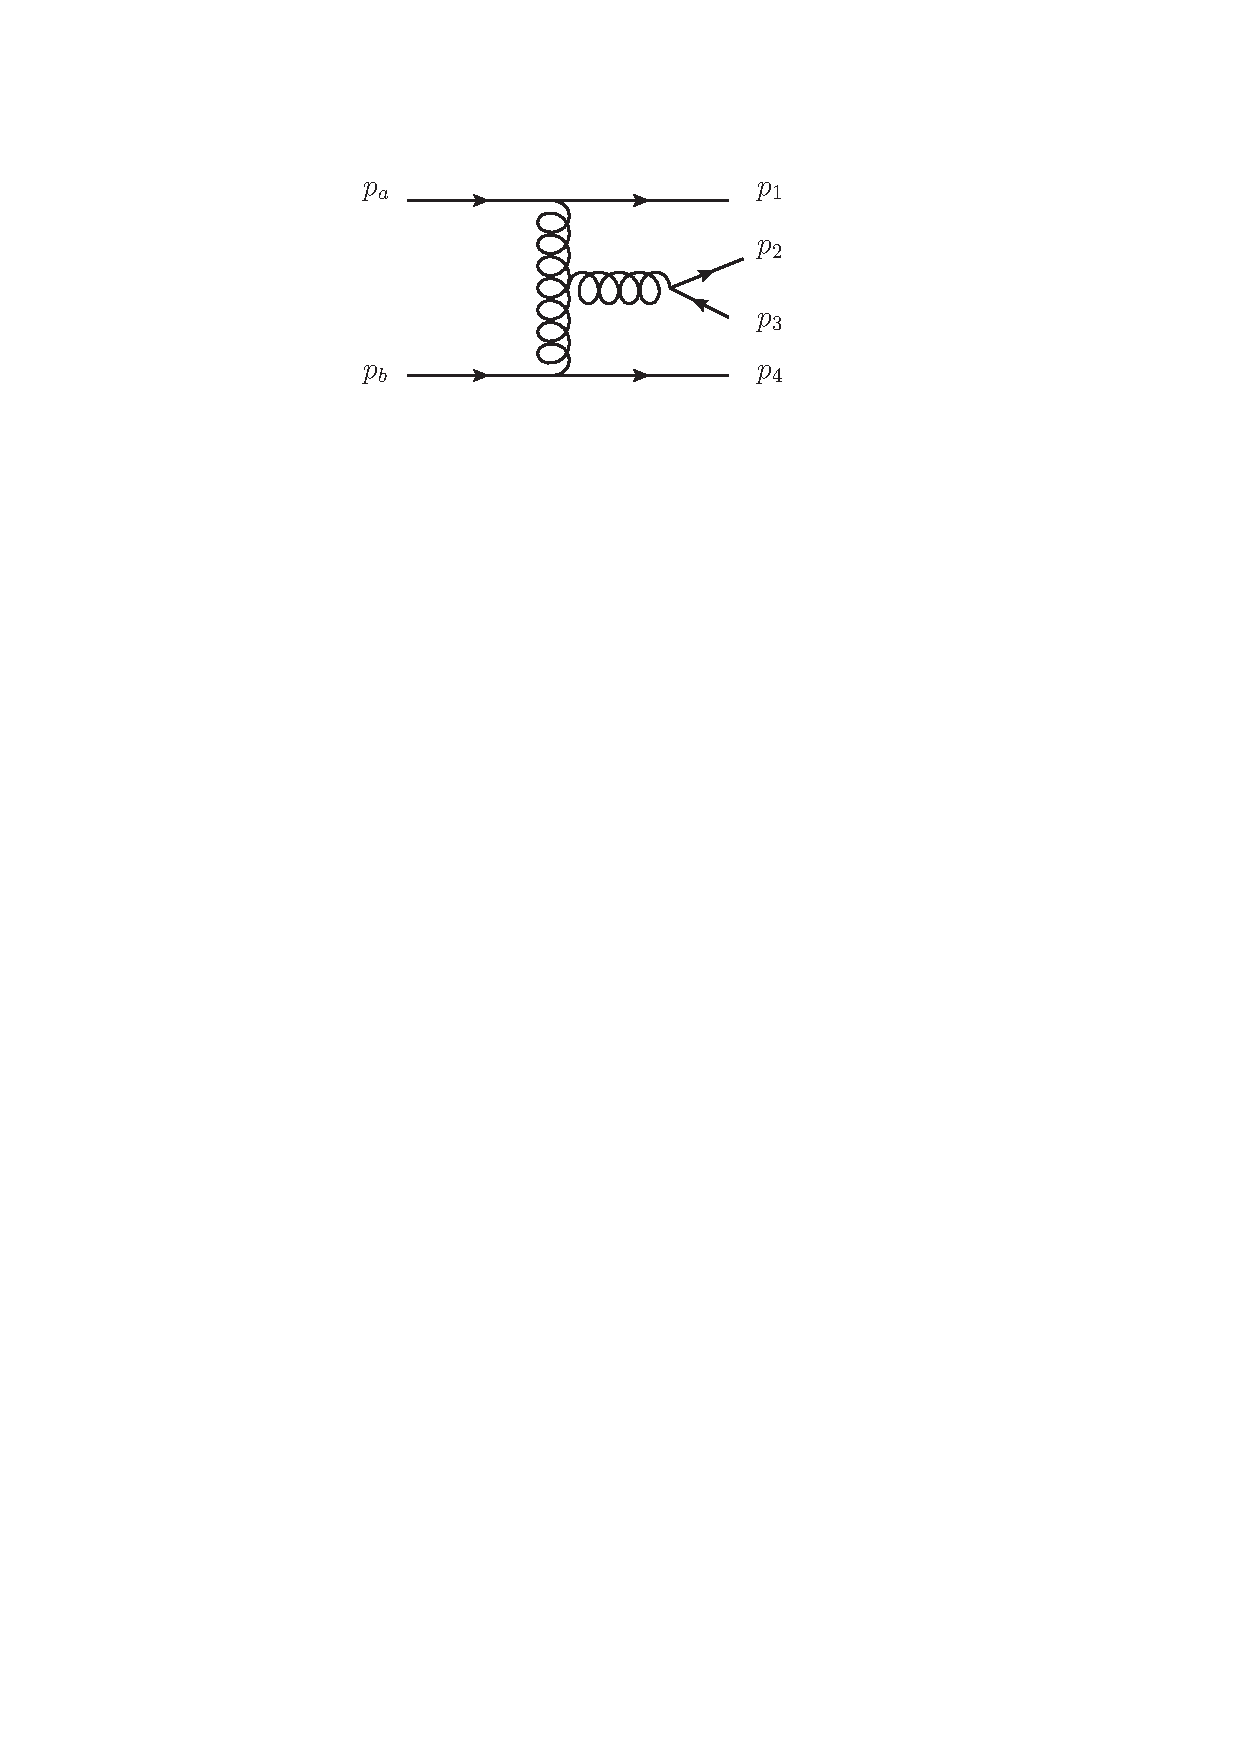
\includegraphics[scale=0.65]{Images/4j_middle_qqg.pdf}}
\subfloat{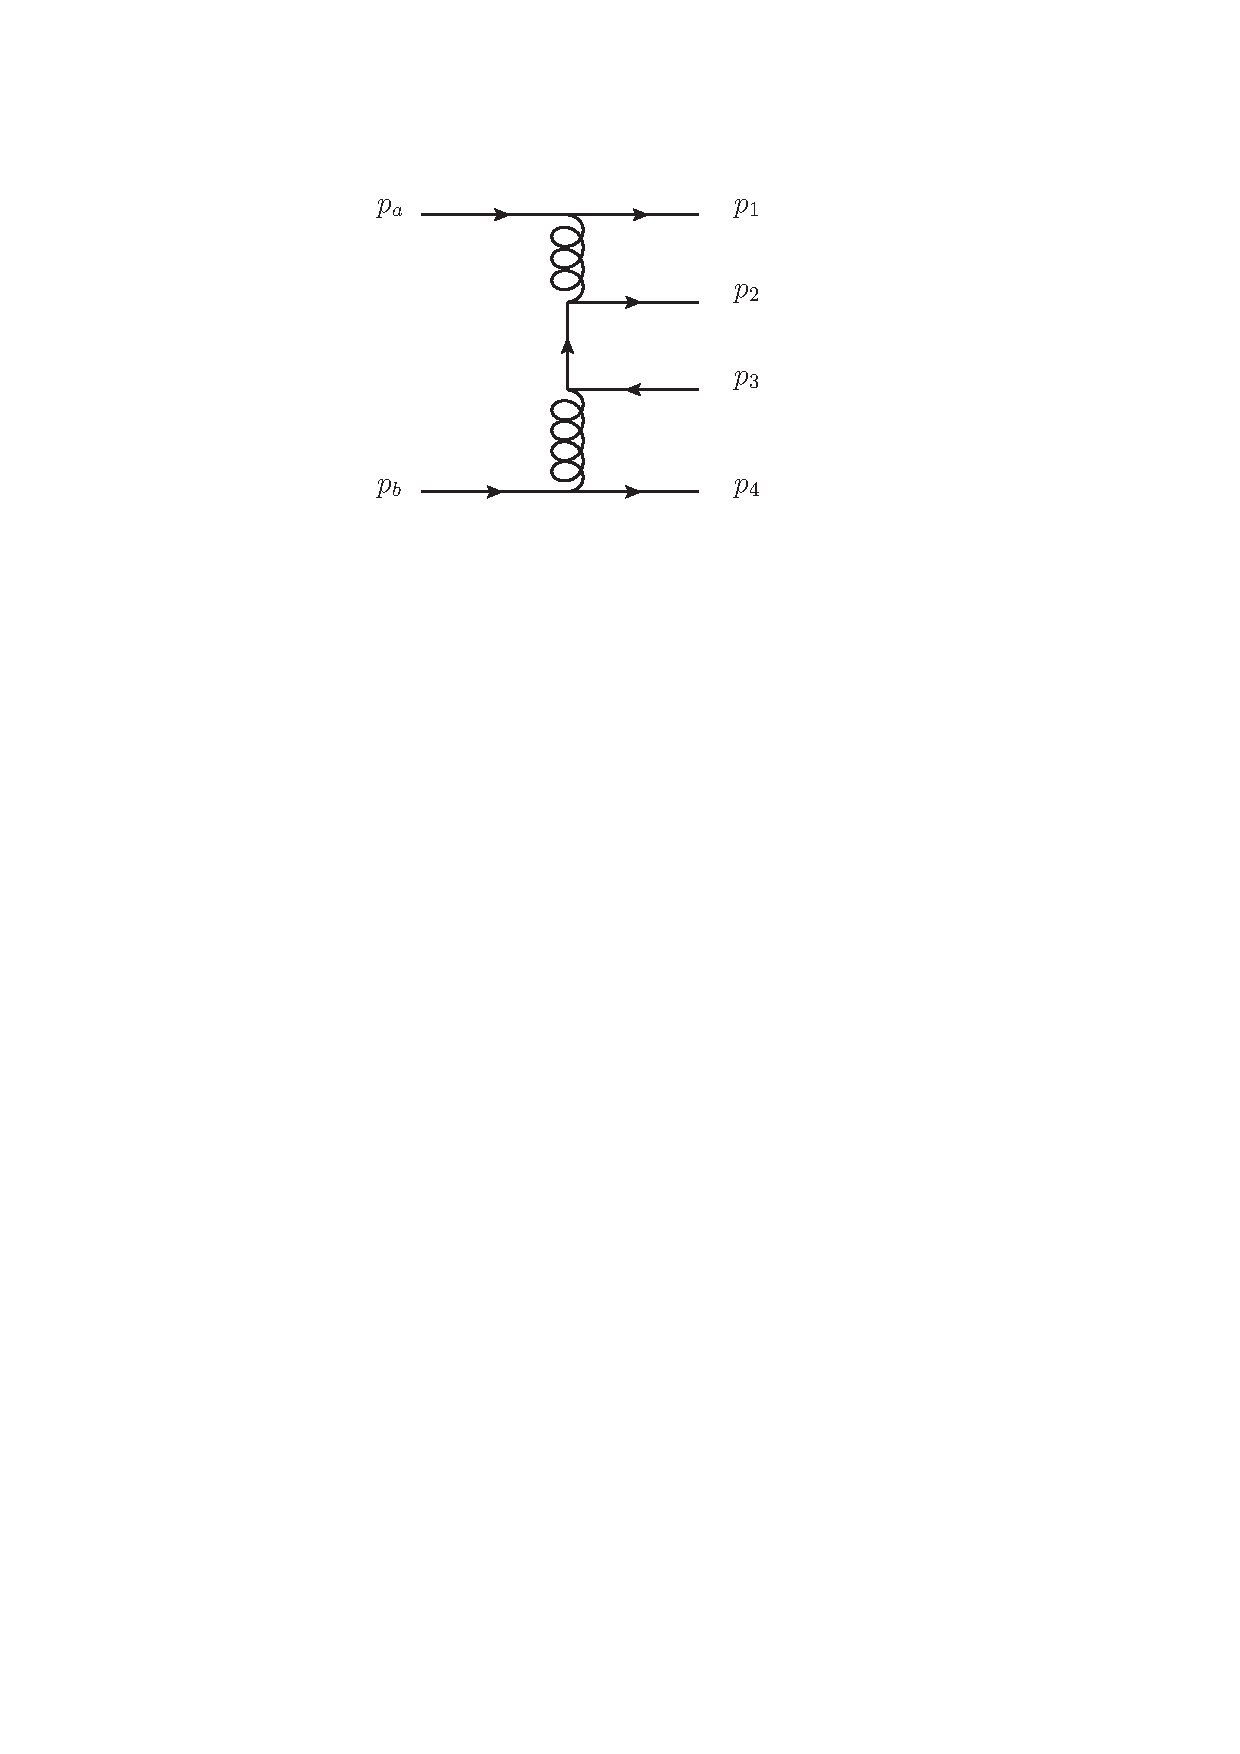
\includegraphics[scale=0.65]{Images/4jet_qprop.pdf}} \\
\subfloat{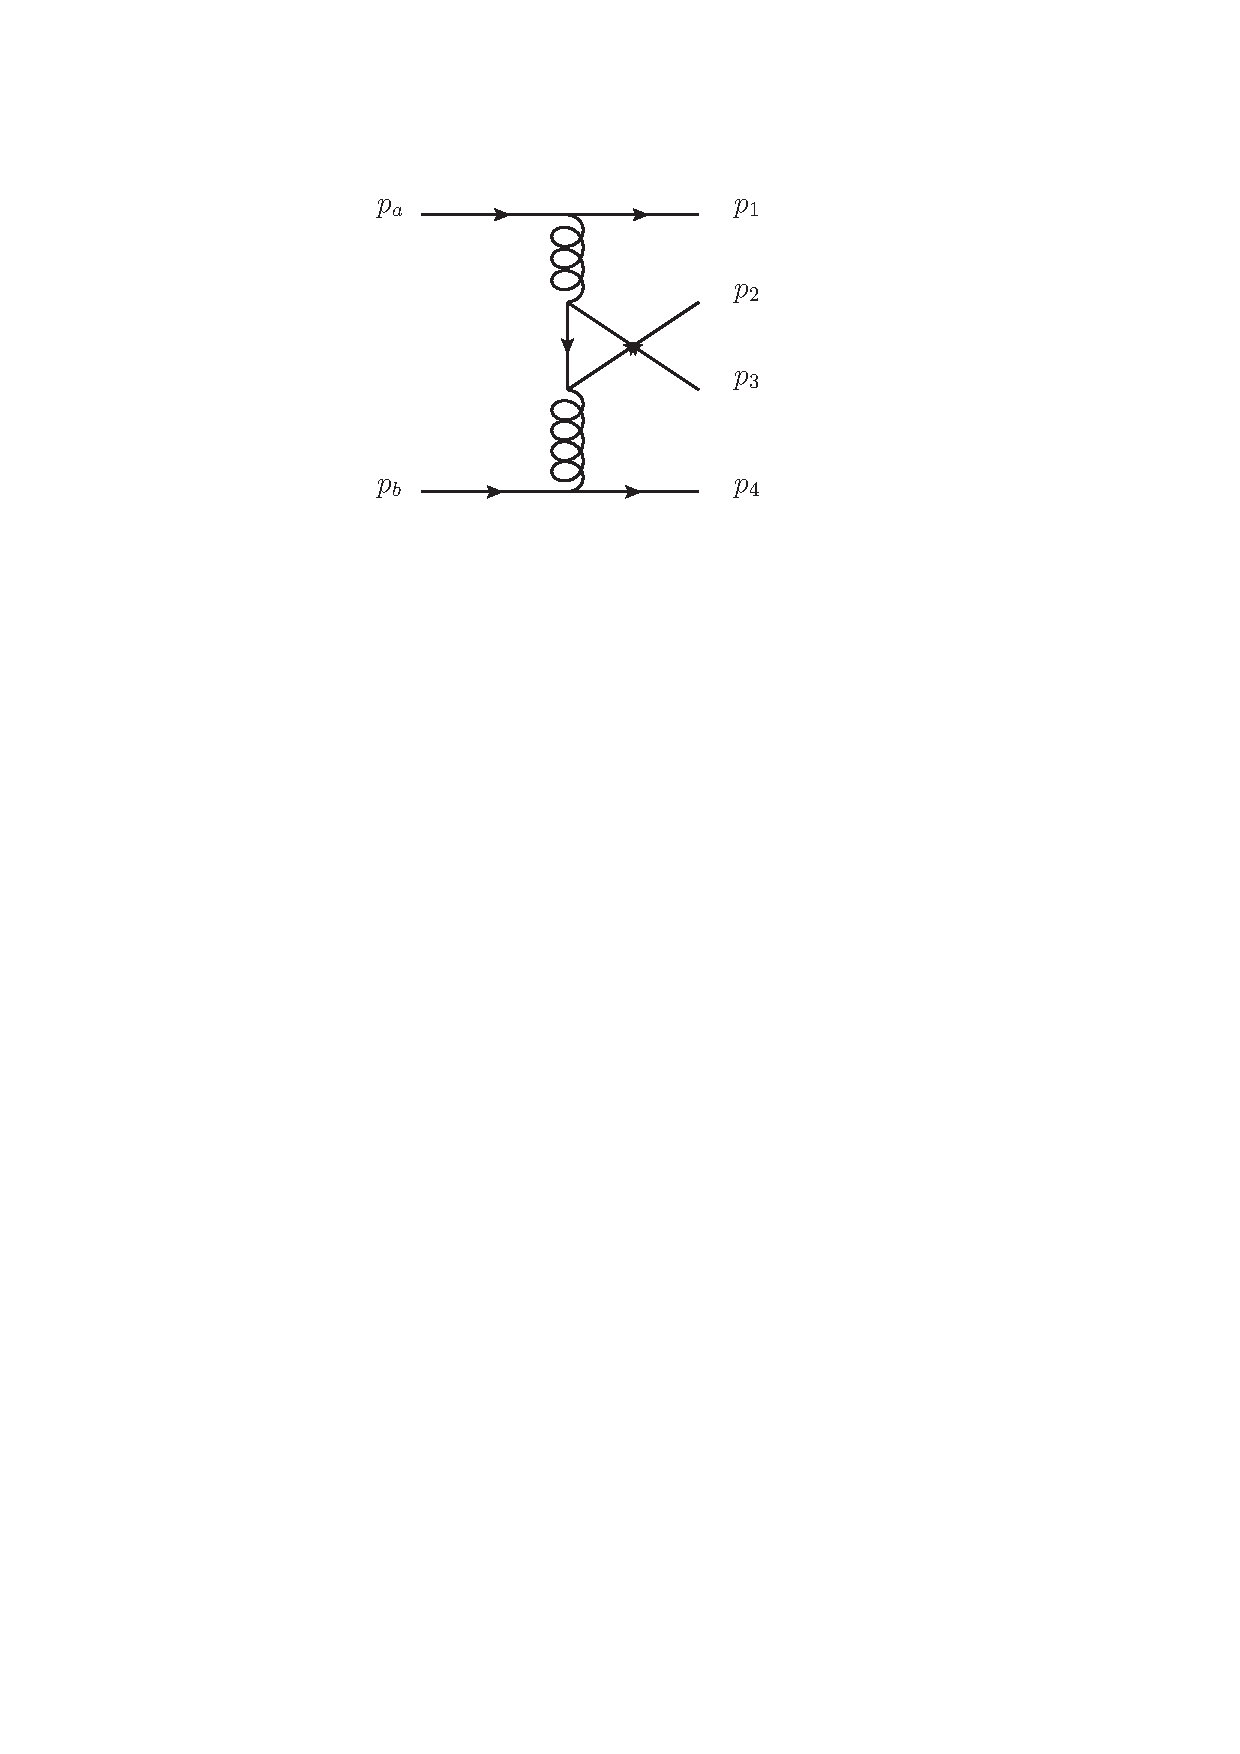
\includegraphics[scale=0.65]{Images/4jet_qprop_crossed.pdf}}
\caption{All LO graphs for $qq' \to qQ\bar{Q}q'$.}
\label{fig:qq_qQQq_graphs}
\end{figure}

It is immediately clear that this diagram will not factorise into our desired form, so we expand the square bracket as a spinor chain again to attempt to make some approximations;

\begin{equation}
\frac{1}{s_{12} + s_{13} + s_{23}} \left(\matel{1}{\mu}{1}\matel{1}{\rho}{a} + \matel{1}{\mu}{2} \matel{2}{\rho}{a} + \matel{1}{\mu}{3} \matel{3}{\rho}{a} \right).
\end{equation}

Depending on the helicities, either the second or third term in this bracket is identically zero when contracted with the quark current $\matel{2}{\mu}{3}$. Once more, we can use a scaling argument to eliminate other terms in this string. The first term contracted with $\matel{2}{\mu}{3}$ will scale as $\sqrt{s_{12} s_{13}}$ regardless of helicity choices. For the other non-zero term, the scaling will be like $\sqrt{s_{23} s_{12}}$. We have no requirement that $s_{23}$ be large but all other invariants there are large and thus we can approximate the sub-amplitude by keeping the first term only; 

\begin{equation}
iM_1 \approx  \frac{- i g_s^4 T^e_{1q}T^g_{qa}T^e_{23}T^g_{4b}}{s_{23} \hat{t}_3 (s_{12} + s_{13})} \matel{1}{\rho}{a} \matel{4}{\rho}{b} \times 2p_1^\mu \matel{2}{\mu}{3}.
\end{equation} 

The next graph is very similar to the previous and so the calculation proceeds in the same fashion as before. We will then skip to the final expression (having again made the approximation) which is;

\begin{equation}
iM_2 \approx \frac{ i g_s^4 T^g_{1q}T^e_{qa}T^e_{23}T^g_{4b}}{s_{23} \hat{t}_3 (s_{a2}+s_{a3})} \matel{1}{\rho}{a} \matel{4}{\rho}{b}\times 2p_a^\mu \matel{2}{\mu}{3}.
\end{equation}    

The next two graphs where the $q \bar{q}$ is emitted from the $p_4$ and $p_b$ legs is clearly very similar to the previous two results. Because of this, we simply state the result of the calculation here for these amplitudes which for the $p_4$ leg is;

\begin{equation}
iM_3 \approx \frac{-i g_s^4 T^g_{1a} T^e_{4q}T^g_{qb}T^e_{23}}{\hat{t}_1 s_{23}(s_{24}+s_{34})}\matel{1}{\rho}{a} \matel{4}{\rho}{b} \times 2 p_4^\mu \matel{2}{\mu}{3},
\end{equation}

and for the $p_b$ leg is;

\begin{equation}
iM_4 \approx \frac{i g_s^4 T^g_{1a} T^g_{4q} T^e_{qb} T^e_{23}}{\hat{t}_1 s_{23}(s_{2b}+s_{3b})} \matel{1}{\rho}{a} \matel{4}{\rho}{b} \times 2 p_b^\mu \matel{2}{\mu}{3}.
\end{equation}

The remaining graphs are already $t$-channel factorised and so we know that we can include them exactly. The next diagram where the $q \bar{q}$ emission is off of the $t$-channel gluon propagator has the exact expression;

\begin{equation}
\begin{split}
iM_5 &= \frac{g_s^4 T^g_{1a} f^{geg'}T^{g'}_{4b}T^e_{23}}{\hat{t}_1 s_{23} \hat{t}_3} \left((q_1 + p_2 + p_3)^\lambda \eta^{\nu \sigma} + (q_3 - p_2 -p_3)^\nu \eta^{\sigma \lambda} - (q_1 + q_3)^\sigma \eta^{\nu \lambda} \right) \\
& \left[\bar{u}_1 \gamma_\nu u_a \right]  \left[\bar{u}_4 \gamma_\lambda u_b \right] \left[\bar{u}_2 \gamma_\sigma u_3 \right].
\end{split}
\end{equation}

The final two diagrams both have quark propagators. They have the exact expressions;

\begin{equation}
iM_6 = \frac{i g_s^4 T^g_{1a} T^{g}_{2q} T^{g'}_{q3}  T^{g'}_{4b}}{\hat{t}_1 \hat{t}_2 \hat{t}_3}\left[\bar{u}_1 \gamma^\mu u_a \right] \left[\bar{u}_4 \gamma^\sigma u_b \right] \left[\bar{u}_2 \gamma_\mu(\slashed{p}_a - \slashed{p}_1 -\slashed{p}_2) \gamma_\sigma u_3 \right],
\end{equation}

and;

\begin{equation}
iM_7 = \frac{-i g_s^4 T^g_{1a} T^{g'}_{2q} T^{g}_{q3}  T^{g'}_{4b}}{\hat{t}_1 \tilde{t}_2 \hat{t}_3}\left[\bar{u}_1 \gamma^\mu u_a \right] \left[\bar{u}_4 \gamma^\sigma u_b \right] \left[\bar{u}_2 \gamma_\sigma(\slashed{p}_a - \slashed{p}_1 -\slashed{p}_3) \gamma_\mu u_3 \right],
\end{equation}
respectively, where $\tilde{t}_2 = (p_a-p_1-p_3)^2$. 

Since the High Energy limit here still implies $p_a \sim p_1$ and $p_b \sim p_4$, we can approximately combine both $M_1$ with $M_2$ and $M_3$ with $M_4$. Doing the former yields;

\begin{equation}
i(M_1 + M_2) \approx \frac{ C_1 g_s^4}{s_{23} \hat{t}_3 (s_{a2} + s_{a3})} \matel{1}{\rho}{a} \matel{4}{\rho}{b} \times 2 p_a^\sigma \matel{2}{\sigma}{3},
\end{equation} 

where we have defined:

\begin{equation}
C_1 = T^e_{1q}T^g_{qa} T^e_{23}T^g_{4b} - T^g_{1q}T^e_{qa}T^e_{23}T^g_{4b} = f^{egc}T^c_{1a}T^e_{23}T^g_{4b},
\end{equation}

and a similar process on $M_3$ and $M_4$ grants;

\begin{equation}
i(M_3 + M_4) \to \frac{-C_1 g_s^4}{s_{23}\hat{t}_1 (s_{b2}+s_{b3})} \matel{1}{\rho}{a} \matel{4}{\rho}{b} \times 2 p_b^\sigma \matel{2}{\sigma}{3}. 
\end{equation}

We are then in a position to combine all graphs together and derive our effective vertex $X^{\mu \nu}$;

\begin{equation}
\begin{split}
X^{\mu \nu} &=  \frac{C_1}{s_{23}}\left(\eta^{\mu \nu}\left(2 p_a^\sigma \left( \frac{q_1^2}{s_{a2}+s_{a3}} \right) - 2 p_b^\sigma \left(\frac{q_3^2}{s_{b_2}+s_{b3}} \right) \right)+ V_{3g}^{\mu \nu \sigma} \right)\matel{2}{\sigma}{3} \\
&+ \frac{i C_2}{\hat{t}_2} X_{qprop}^{\mu \nu} - \frac{i C_3}{\tilde{t}_2} X_{crossed}^{\mu \nu},
\end{split}
\end{equation}

where we have defined the following expressions:

\begin{subequations}
\begin{align}
V_{3g}^{\mu \nu \sigma} &= (q_1 + p_2 + p_3)^\nu \eta^{\mu \sigma} + (q_3 - p_2 -p_3)^\mu \eta^{\sigma \nu} - (q_1 + q_3)^\sigma \eta^{\mu \nu} \\
C_2 &= T^g_{1a}T^g_{2q}T^{g'}_{q3}T^{g'}_{4b} \\
C_3 &= T^g_{1a}T^{g'}_{2q}T^g_{q3}T^{g'}_{4b} \\
X_{qprop}^{\mu \nu} &= \bar{u}_2 \gamma^\mu (\slashed{q}_1 - \slashed{p}_2)\gamma^\nu u_3 \\
X_{crossed}^{\mu \nu} &=\bar{u}_2 \gamma^\nu (\slashed{q}_1 - \slashed{p}_3)\gamma^\mu u_3.
\end{align}
\end{subequations}

In fact, since we assumed $p_a \sim p_1$ and $p_b \sim p_4$ in deriving this form, we can go one step further and reinstate this symmetry so that our final vertex looks like:

\begin{equation}
\begin{split}
X^{\mu \nu} &= \frac{C_1}{s_{23}} \left(\eta^{\mu \nu} X_{sym}^\sigma + V^{\mu \nu \sigma}_{3g} \right) \matel{2}{\sigma}{3} \\
&+ \frac{i C_2}{\hat{t}_2} X^{\mu \nu}_{qprop} - \frac{i C_3}{\tilde{t}_2} X^{\mu \nu}_{crossed},
\end{split}
\end{equation}

with:

\begin{equation}
\begin{split}
X_{sym}^\sigma &= p_a^\sigma \left( \frac{q_1^2}{s_{a2}+s_{a3}} \right) + p_1^\sigma \left( \frac{q_1^2}{s_{12}+s_{13}} \right) \\
&- p_b^\sigma \left( \frac{q_3^2}{s_{b2}+s_{b3}} \right) - p_4^\sigma \left( \frac{q_3^2}{s_{42}+s_{43}} \right).
\end{split}
\end{equation}

We have intentionally used the notation of $q^2$ rather than $\hat{t}$ to make it clear that this invariant is the invariant formed from the mass of the propagator entering into the effective vertex. Once extra emissions are added, the $\hat{t}$ notation can be misleading. With this, we now have the complete expression for the effective central $q\bar{q}$ vertex. 

\subsection{Checks and Verifications of Amplitudes}

In order to check the derivation of these amplitudes, we will explicitly investigate how they behave in the MRK limit. We discussed before that we expect them to be suppressed by the invariant $s_{q\bar{q}}$ with respect to the leading FKL configurations at the $|M|^2$ level. Since the FKL amplitudes behaved as $\hat{s}^2$ at the $|M|^2$ level, we should see a systematic dying off of these new amplitudes if we plot $|M|^2/\hat{s}^2$ and furthermore multiplication of $s_{q \bar{q}}$ should combat this suppression. In these amplitudes, we have a more complicated colour structure than we did before, with each effective vertex depending on three. At the $|M|^2$ level, we must ensure to deal with this correctly when performing the colour sum. This is done by splitting up the vertices into sub-vertices, each one of which being associated with one colour factor. For example;

\begin{equation}
Q^{\mu \nu} = C_1 Q^{\mu \nu}_1 + C_2 Q^{\mu \nu}_2 + C_t Q^{\mu \nu}_t,
\end{equation}

which will allows us to calculate the squared amplitude as (the colour sum is implicitly performed);

\begin{equation}
\begin{split}
|M_{qg \to qQ\bar{Q}}|^2 &\sim \frac{1}{24} \bigg(|C_1 M_{Q_1}|^2 + |C_2 M_{Q_2}|^2 + |C_t M_{Q_t}|^2 \\
&+ 2 Re(C_1 C_2^\dagger M_{Q_1}M^\dagger_{Q_2}) + 2 Re(C_1 C_t^\dagger M_{Q_1}M^\dagger_{Q_t}) + 2 Re(C_2 C_t^\dagger M_{Q_2}M^\dagger_{Q_t}) \bigg),
\end{split}
\end{equation}

where the pre-factor comes from the colour averaging factor. We can calculate the $qq' \to qQ\bar{Q}q'$ amplitude in a similar manner. The helicity sum is performed explicitly and the average brings about a further factor of $1/4$ in both cases. In order to check how our matrix element performs against the full leading order result, we plot the value of $|M|^2/\hat{s}^2$ for both approaches (the latter taken from MadGraph) across a slice of phase space. For the $qg \to qQ\bar{Q}$ amplitude, the momenta are chosen such that;

\begin{equation}
\begin{split}
p_1 & = (40 \cosh(\Delta), 0, 40, 40 \sinh(\Delta)), \\
p_2 & = (40 \sqrt{2}, 40 , -40, 0), \\
p_3 & = (40 \cosh(-\Delta), -40, 0, 40 \sinh(-\Delta)), 
\end{split}
\end{equation}

and the results are plotted in figure \ref{fig:qg_qqqx}. We see that the two calculations follow each other very closely and we also see the suppression at large $\Delta$ as we expected. In figure \ref{fig:qg_qqqx_sqqx}, we multiply this result by $s_{q \bar{q}}$ and show that it is indeed this invariant that is suppressing the amplitude in this regime. 

\begin{figure}[H]
\centering
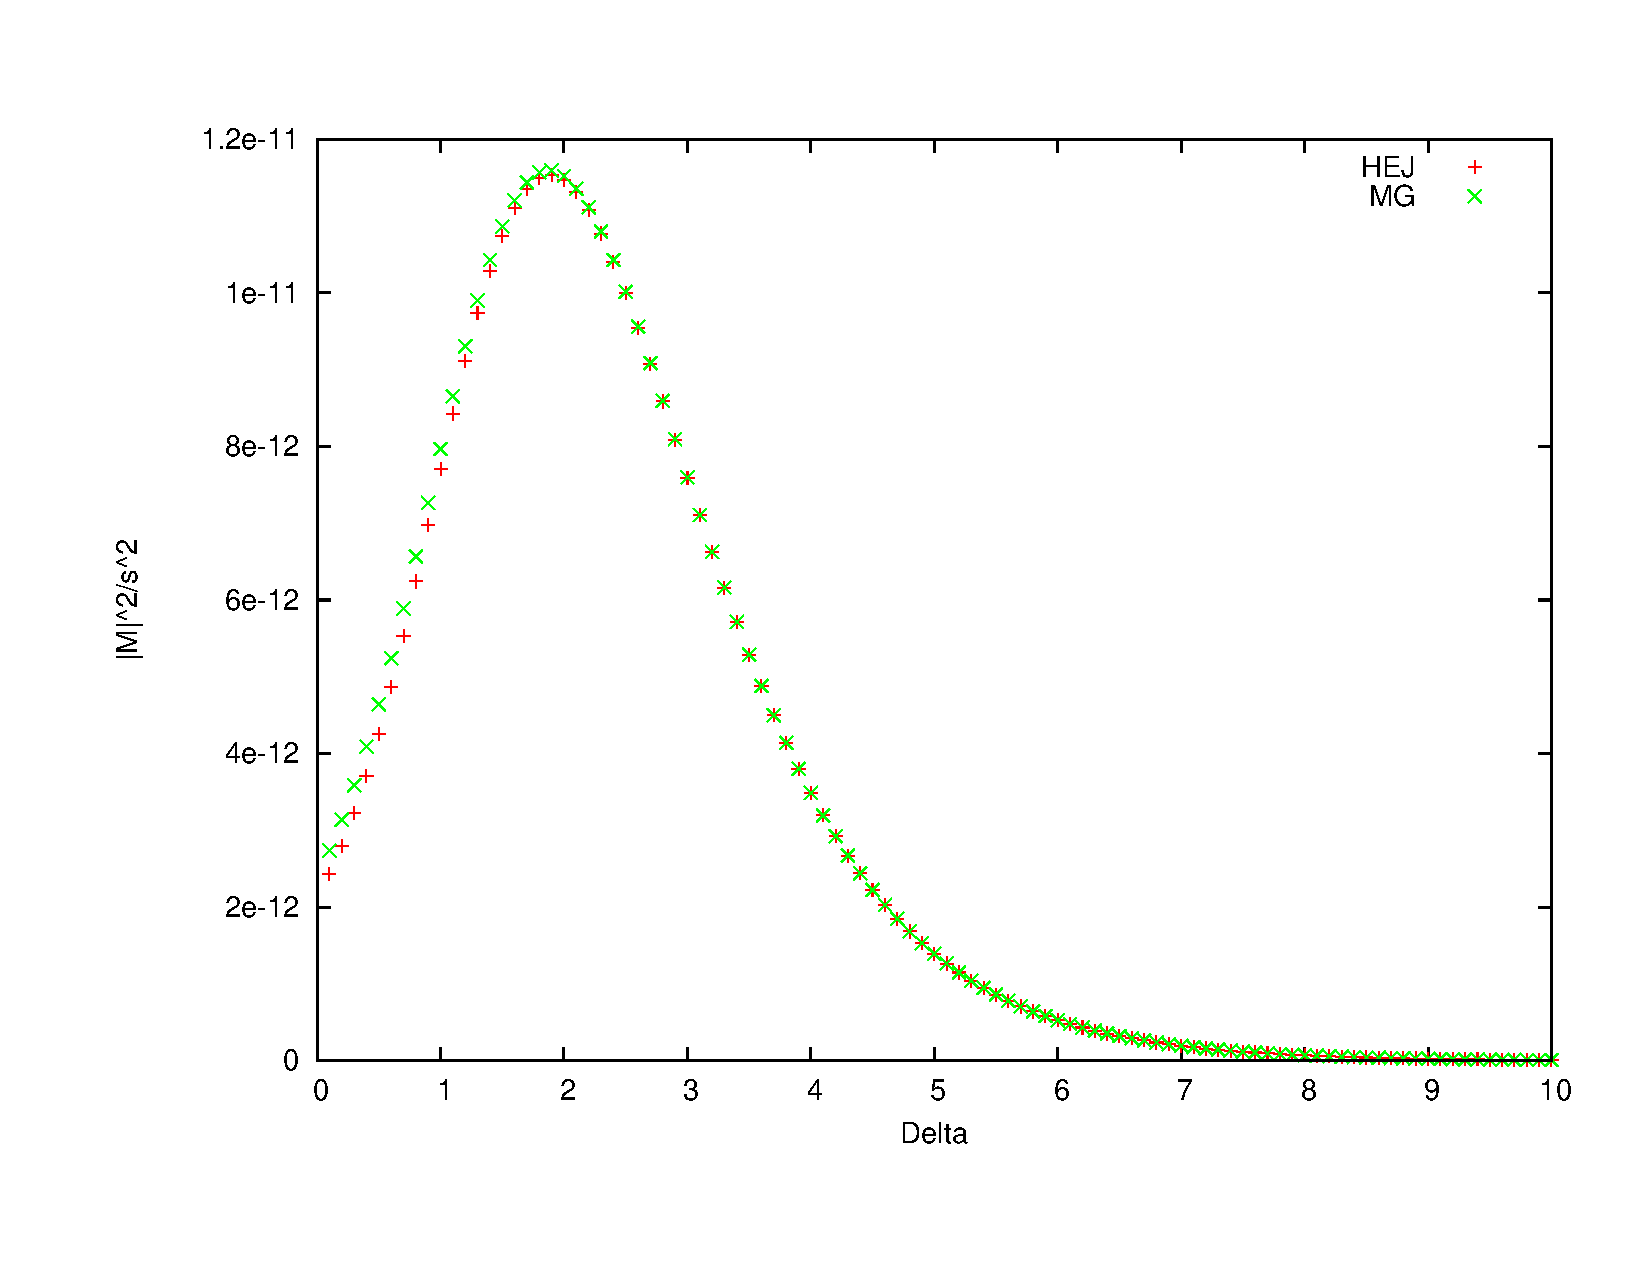
\includegraphics[scale= 0.45]{Images/qg_qqqx.pdf}
\caption{Effective vertex approach to the $qg \to qQ\bar{Q}$ amplitude (red) compared to the full LO (green).}
\label{fig:qg_qqqx}
\end{figure}

\begin{figure}[H]
\centering
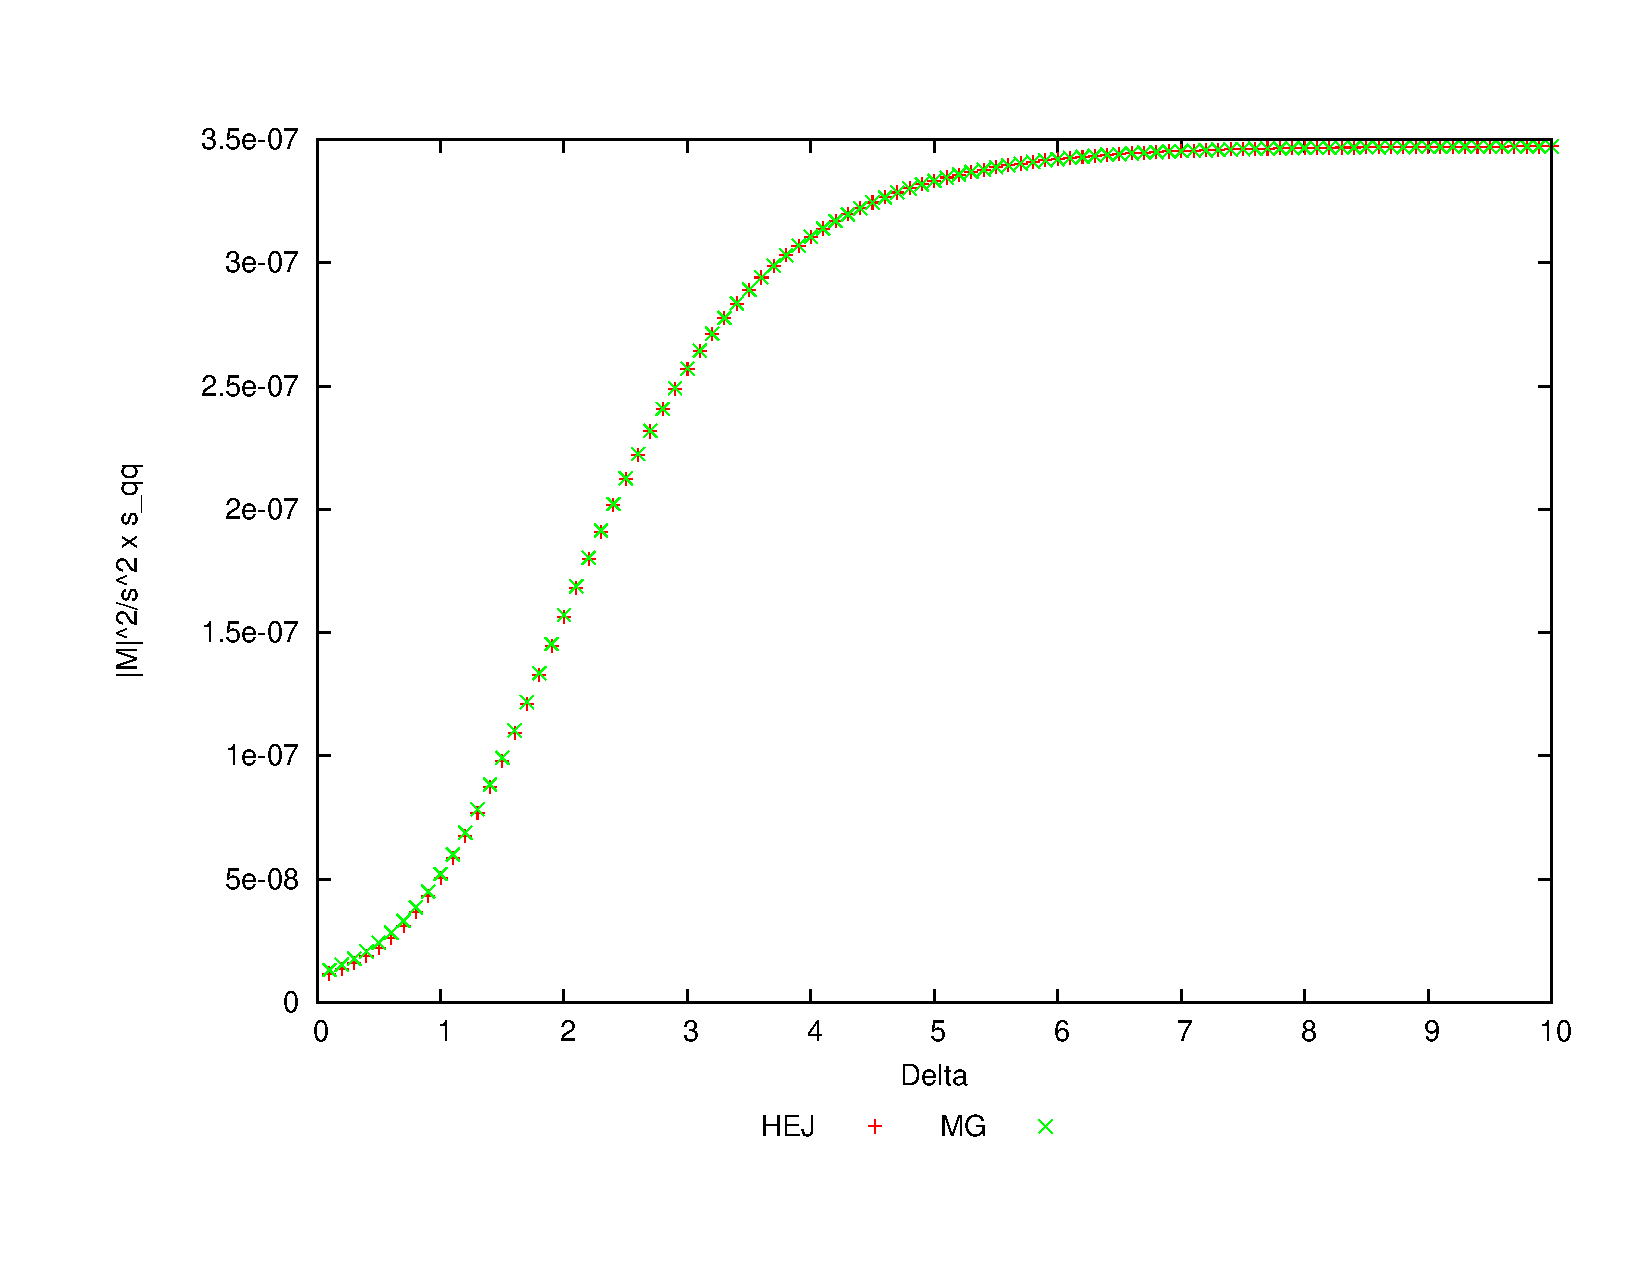
\includegraphics[scale=0.45]{Images/qg_qQQx_sqqx.pdf}
\caption{Effective vertex approach to the $qg \to qQ\bar{Q}$ amplitude (red) compared to the full LO (green) multiplied by the invariant mass of the quark/anti-quark pair.}
\label{fig:qg_qqqx_sqqx}
\end{figure}

We can perform a similar test on the $qq' \to qQ\bar{Q}q'$ amplitude, where we choose the momenta to be;

\begin{equation}
\begin{split}
p_1 & = (40 \cosh(\Delta), 0, 40, 40 \sinh(\Delta)), \\
p_2 & = (40 \cosh(\Delta/3), 40, 0, 40 \sinh(\Delta/3)), \\
p_3 & = (40 \cosh(-\Delta/3), 0, -40, 40 \sinh(-\Delta/3)), \\
p_4 & = (40 \cosh(-\Delta), -40, 0, 40 \sinh(-\Delta)). 
\end{split}
\label{eqn:4jetmom}
\end{equation}

The comparison between our amplitude and the full leading order is shown in figure \ref{fig:qq_qqqq}. We see once more the good agreement between the two across the phase space as well as suppression at large $\Delta$, which figure \ref{fig:qq_qqqq_sqq} shows is due to $s_{q \bar{q}}$. 

\begin{figure}[H]
\centering
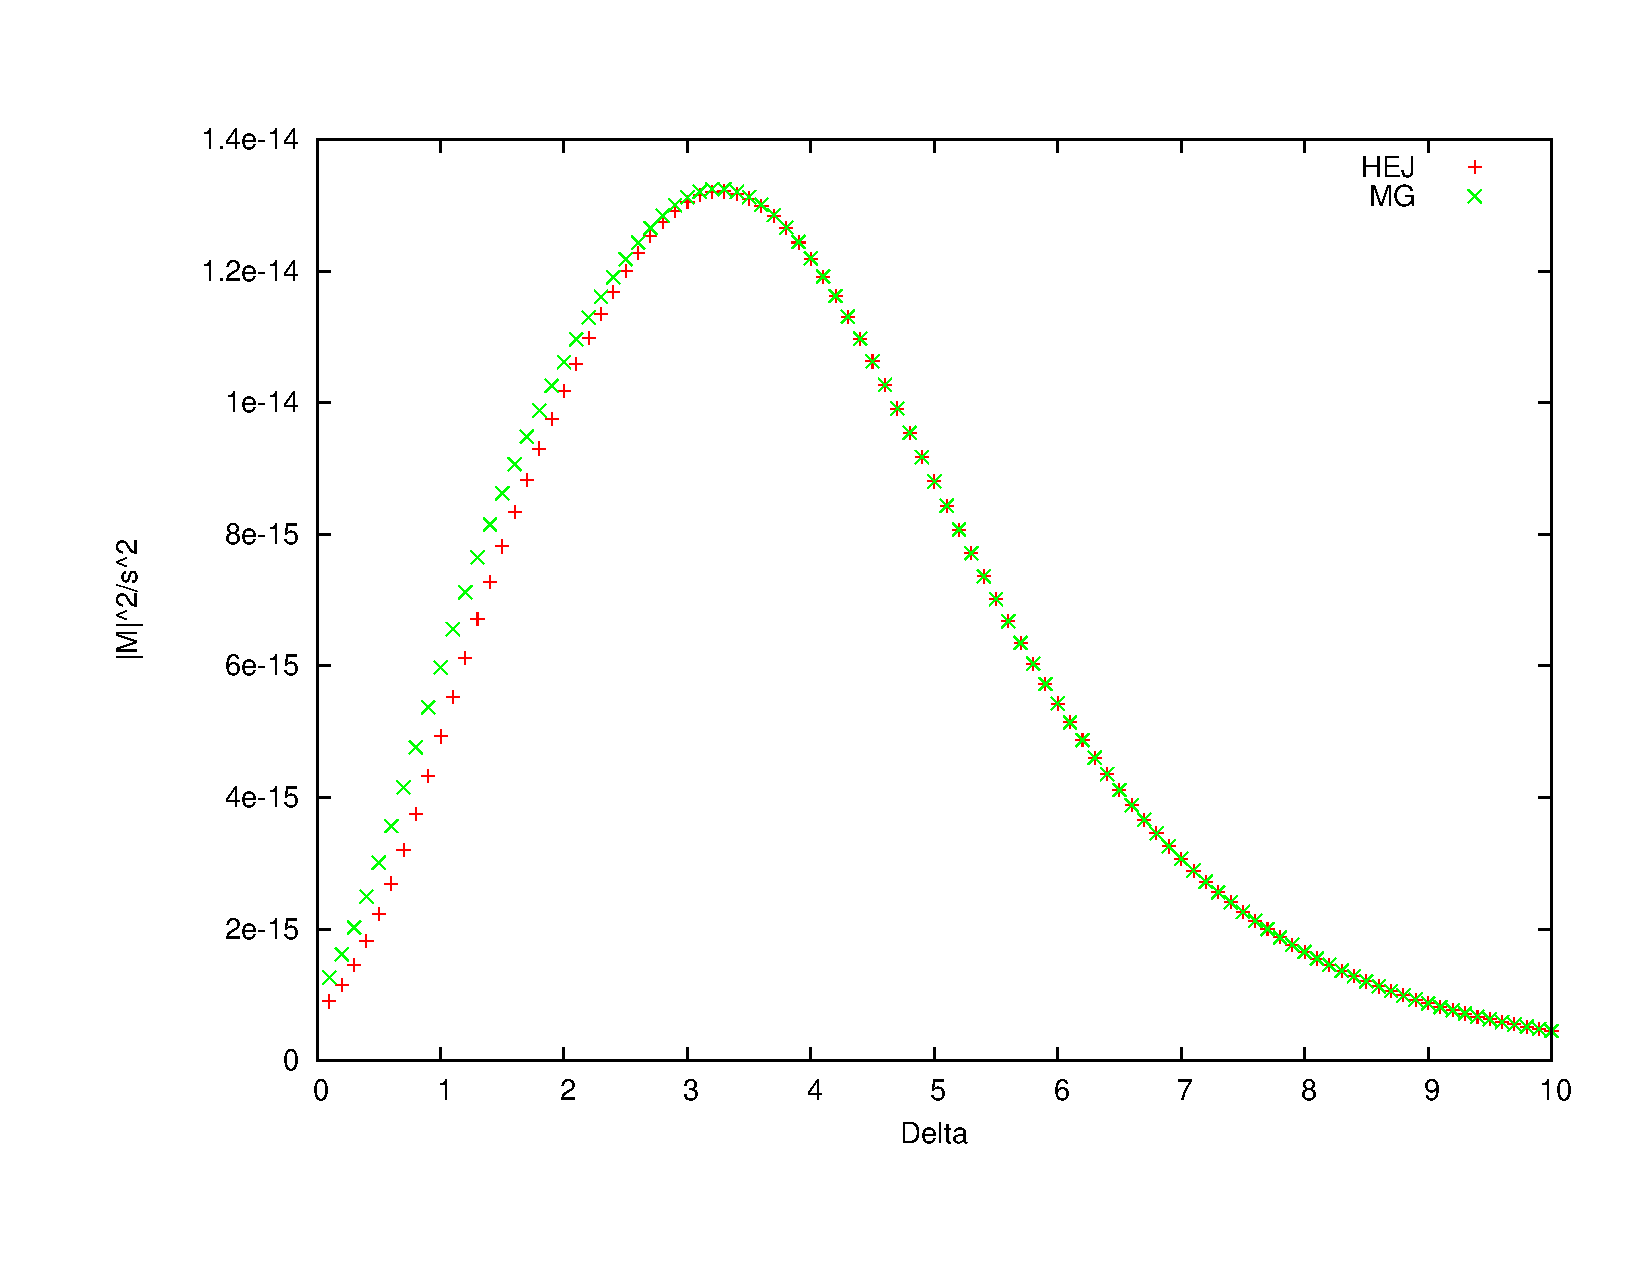
\includegraphics[scale=0.45]{Images/qQ_qqqxQ.pdf}
\caption{Effective vertex approach to the $qq' \to qQ\bar{Q}q'$ amplitude (red) compared to the full LO (green).}
\label{fig:qq_qqqq}
\end{figure}

\begin{figure}[H]
\centering
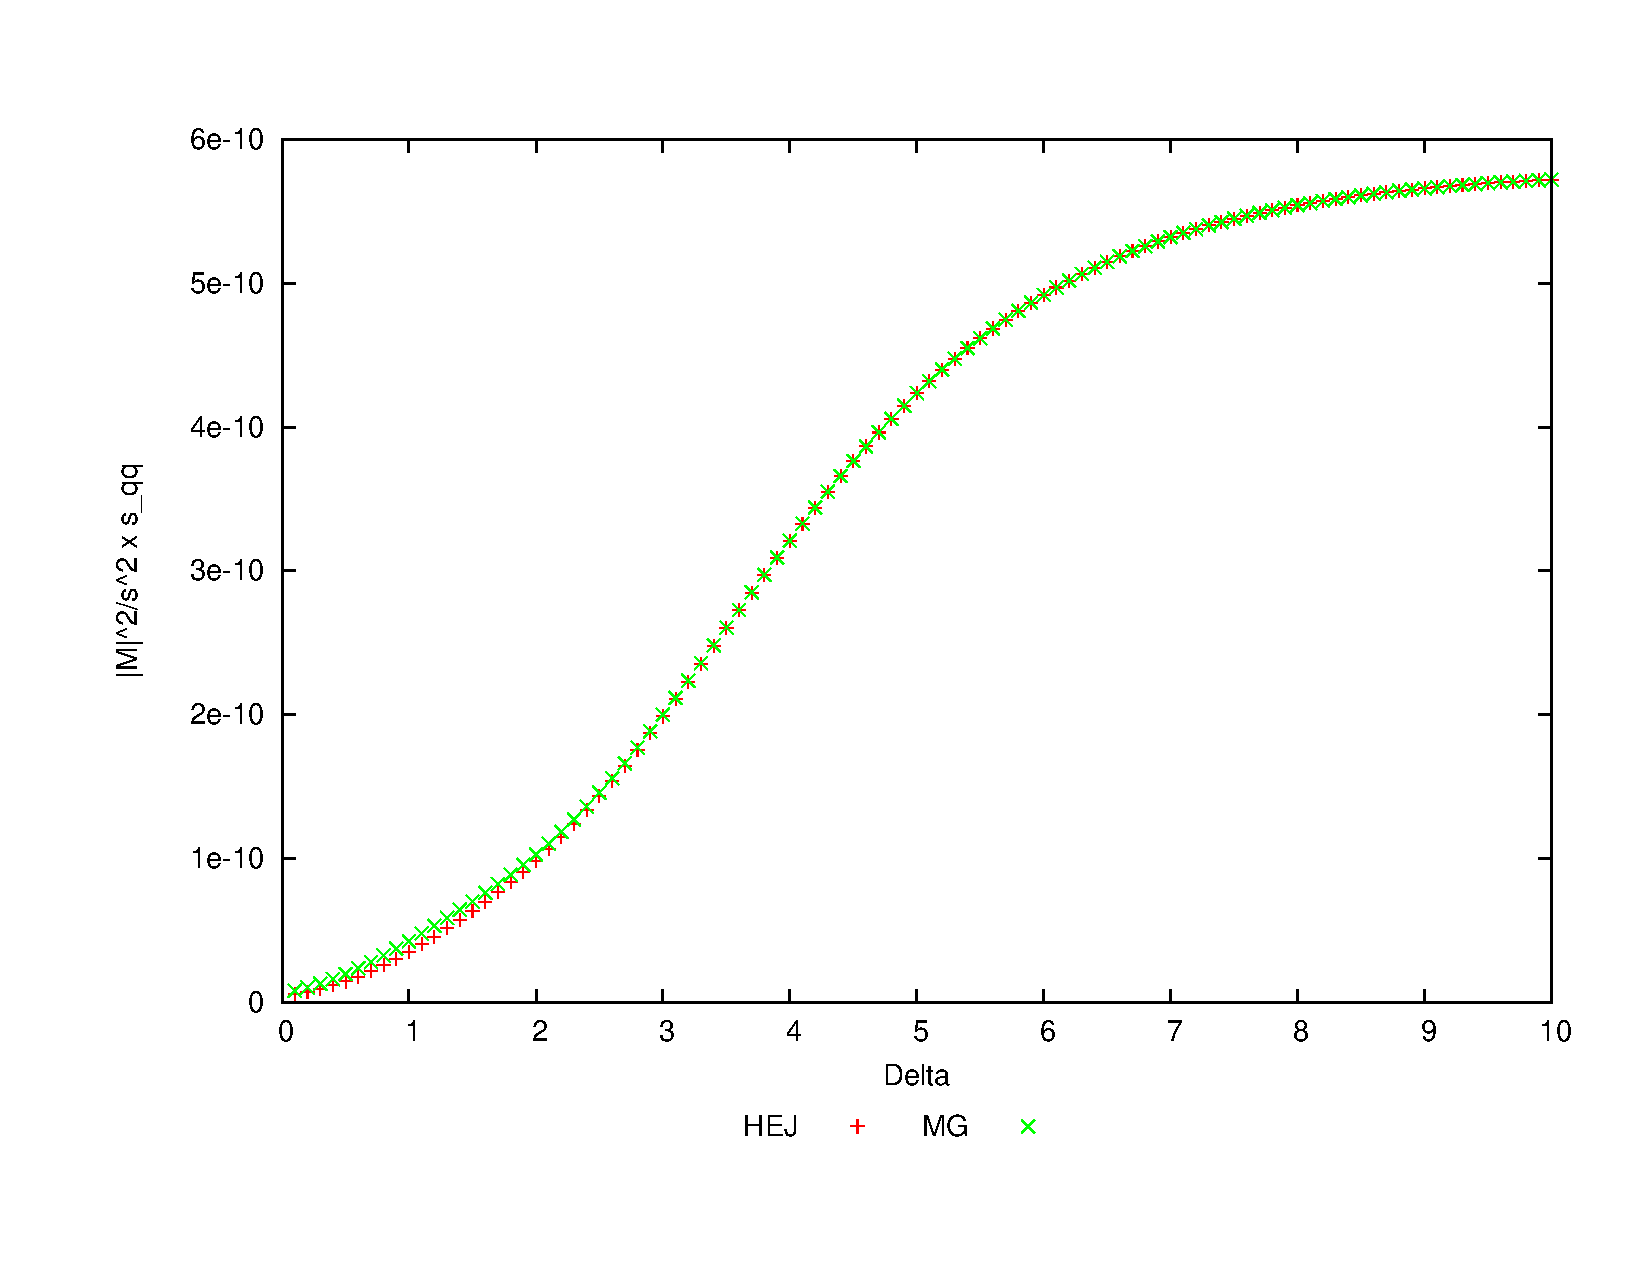
\includegraphics[scale=0.45]{Images/qQ_qqqxQ_sqqx.pdf}
\caption{Effective vertex approach to the $qq' \to qQ\bar{Q}q'$ amplitude (red) compared to the full LO (green) multiplied by the invariant mass of the quark/anti-quark pair.}
\label{fig:qq_qqqq_sqq}
\end{figure}

Given these tests, we are satisfied that these `base' amplitudes work as expected. To extend them, we need to be able to generalise them to an arbitrary incoming state and we need to describe the effect of extra gluon emissions. The first of these, we postulated, can be achieved by a simple multiplication of a colour factor at the $|M|^2$ level and, since this was based on the high energy behaviour of amplitudes, the same idea still applies here. However, for the $qg \to qQ\bar{Q}$ case, we must always require that there is a gluon in the initial state since our vertex is an impact factor for the splitting of a gluon into a quark/anti-quark pair. Therefore, the only extension we need to consider (anti-quarks in the initial state require no alteration) is the replacement of the quark in the initial state with a gluon. Our postulate is that;

\begin{equation}
|M_{gg \to gQ\bar{Q}}|^2 \sim \frac{\tilde{C}_A}{C_F} |M_{qg \to qQ\bar{Q}}|^2,
\end{equation}

and we plot this result (multiplied by $s_{q\bar{q}}$) along with the full leading order in figure \ref{fig:gg_qqq}. The difference between the two lines is minimal and only in the low $\Delta$ regime where it should be expected to be different. We conclude that this method of replacing incoming partons does indeed still hold. For completeness, we also check the $qq' \to qQ\bar{Q}q'$ amplitude, where we can have both $qg$ and $gg$ initial states;

\begin{equation}
\begin{split}
|M_{qg \to qQ\bar{Q}g}|^2 &\sim \frac{\tilde{C}_A}{C_F} |M_{qq' \to qQ\bar{Q}q'}|^2, \\
|M_{gg \to gQ\bar{Q}g}|^2 &\sim \left(\frac{\tilde{C}_A}{C_F}\right)^2 |M_{qq' \to qQ\bar{Q}q'}|^2.
\end{split}
\end{equation}

\begin{figure}[t]
\centering
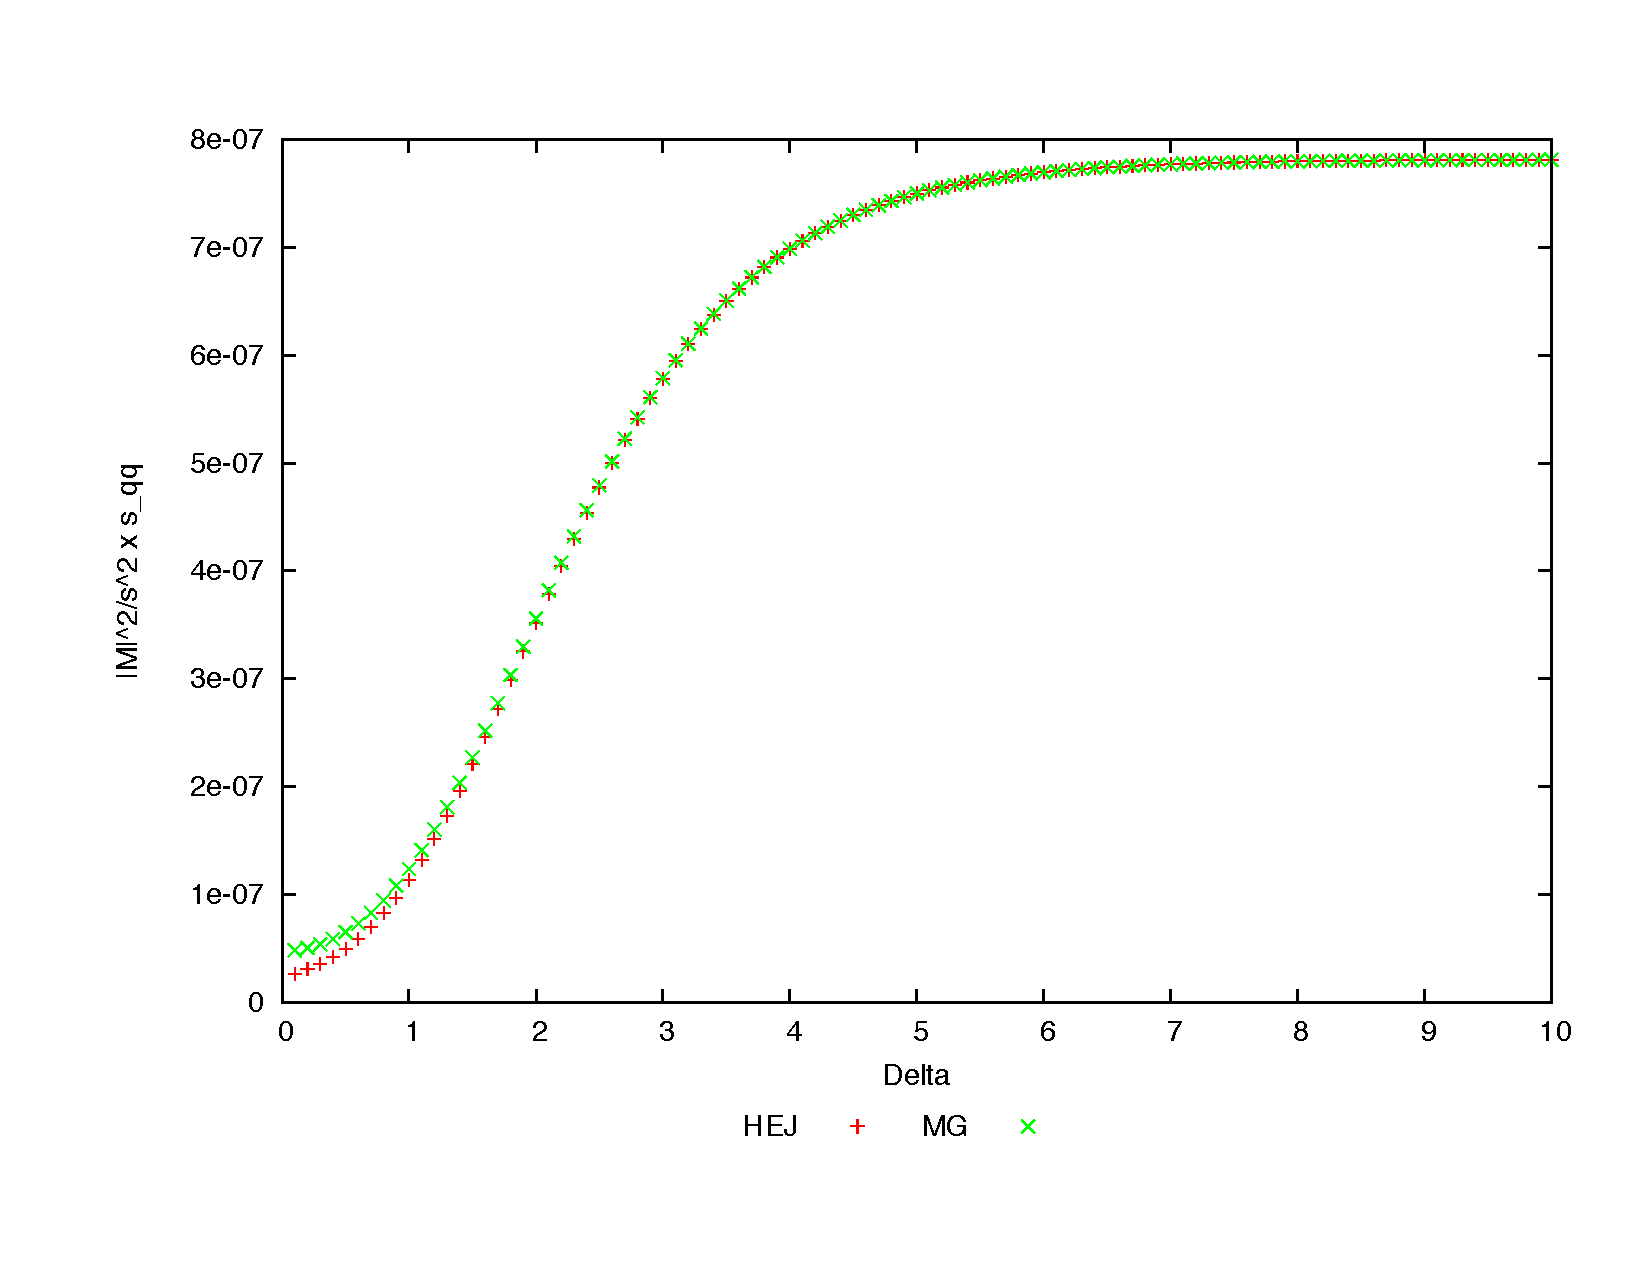
\includegraphics[scale=0.45]{Images/gg_gQQx_sqqx_simplecf.pdf}
\caption{Effective vertex approach to the $gg \to gQ\bar{Q}$ amplitude (red) compared to the full LO (green) multiplied by the invariant mass of the quark/anti-quark pair.}
\label{fig:gg_qqq}
\end{figure}

The comparison to the full leading order of these amplitudes (multiplied by $s_{q\bar{q}}$) is shown in figures \ref{fig:qg_qqqg} and \ref{fig:gg_gqqg} respectively. 

\begin{figure}[H]
\centering
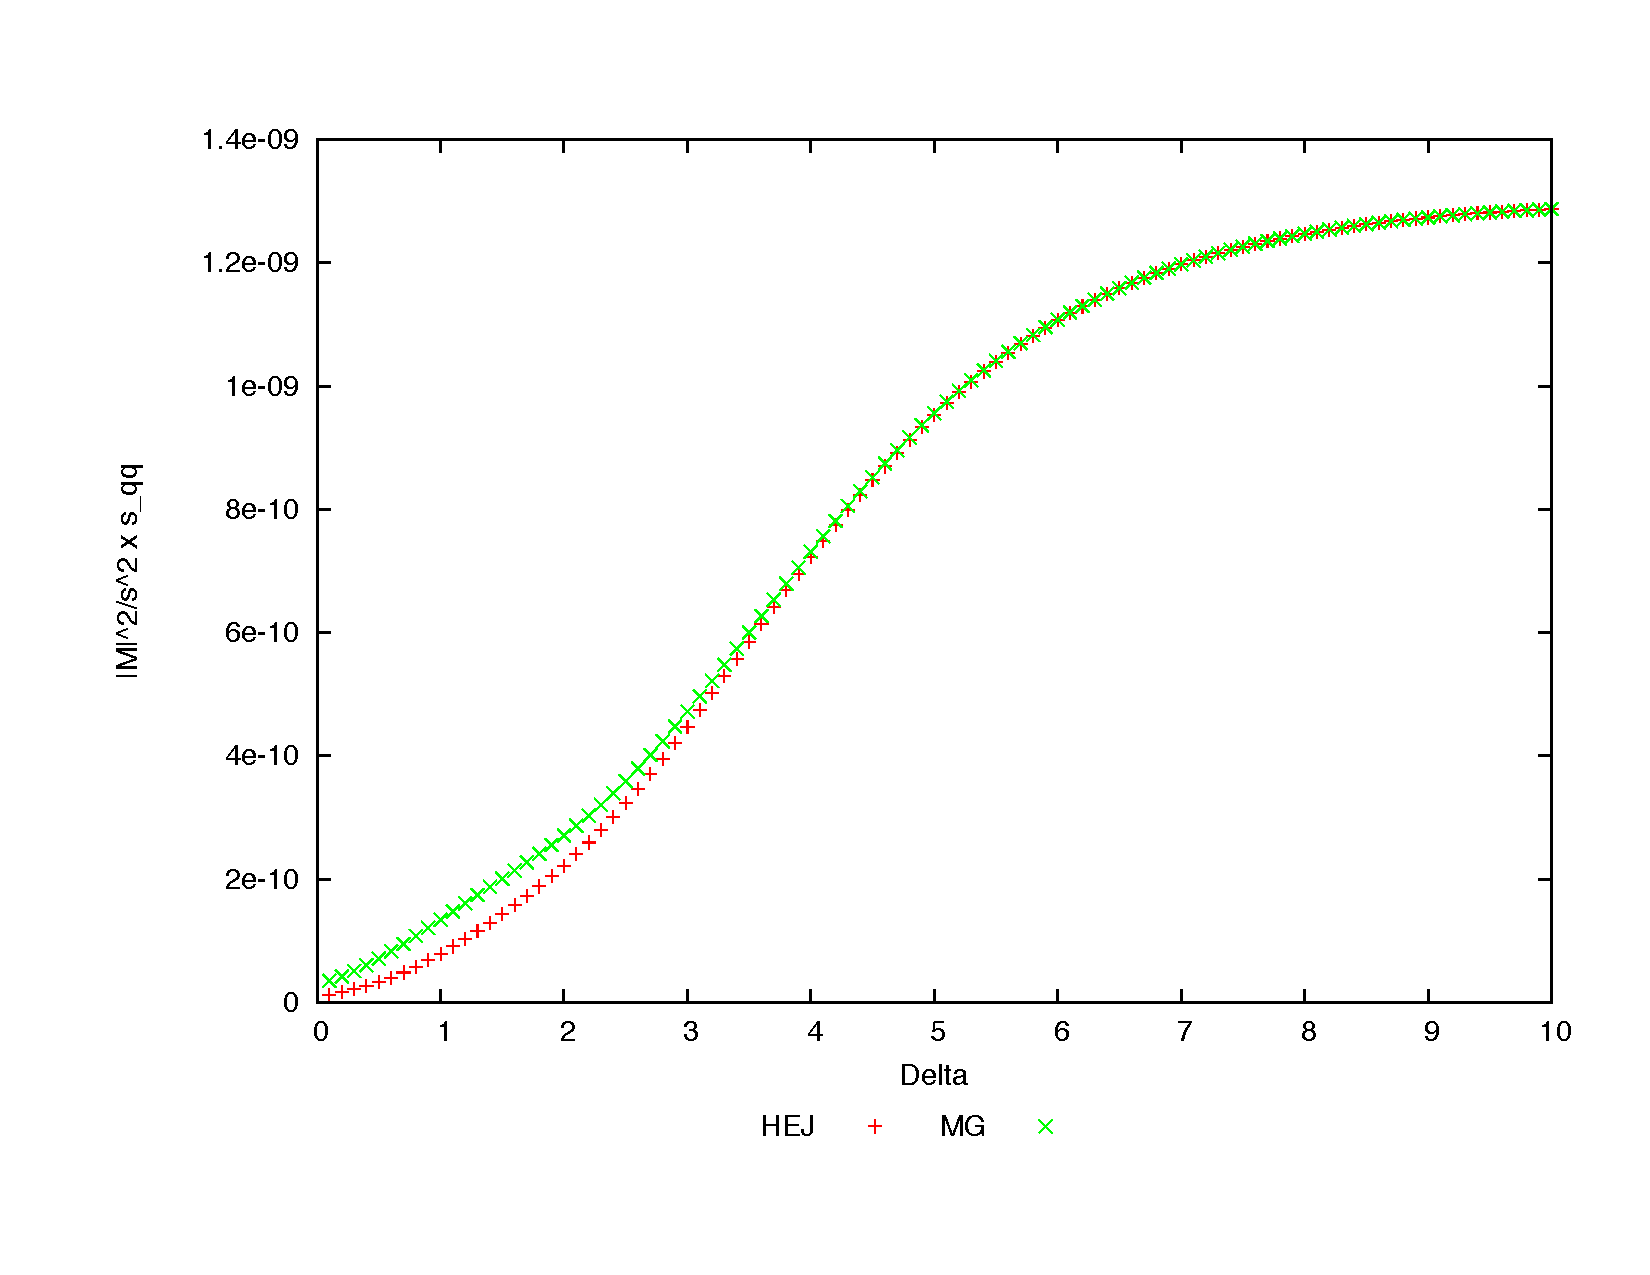
\includegraphics[scale=0.47]{Images/qg_qqqxg_sqq_simplecf.pdf}
\caption{Effective vertex approach to the $qg \to qQ\bar{Q}g$ amplitude (red) compared to the full LO (green) multiplied by the invariant mass of the quark/anti-quark pair.}
\label{fig:qg_qqqg}
\end{figure}

\begin{figure}[H]
\centering
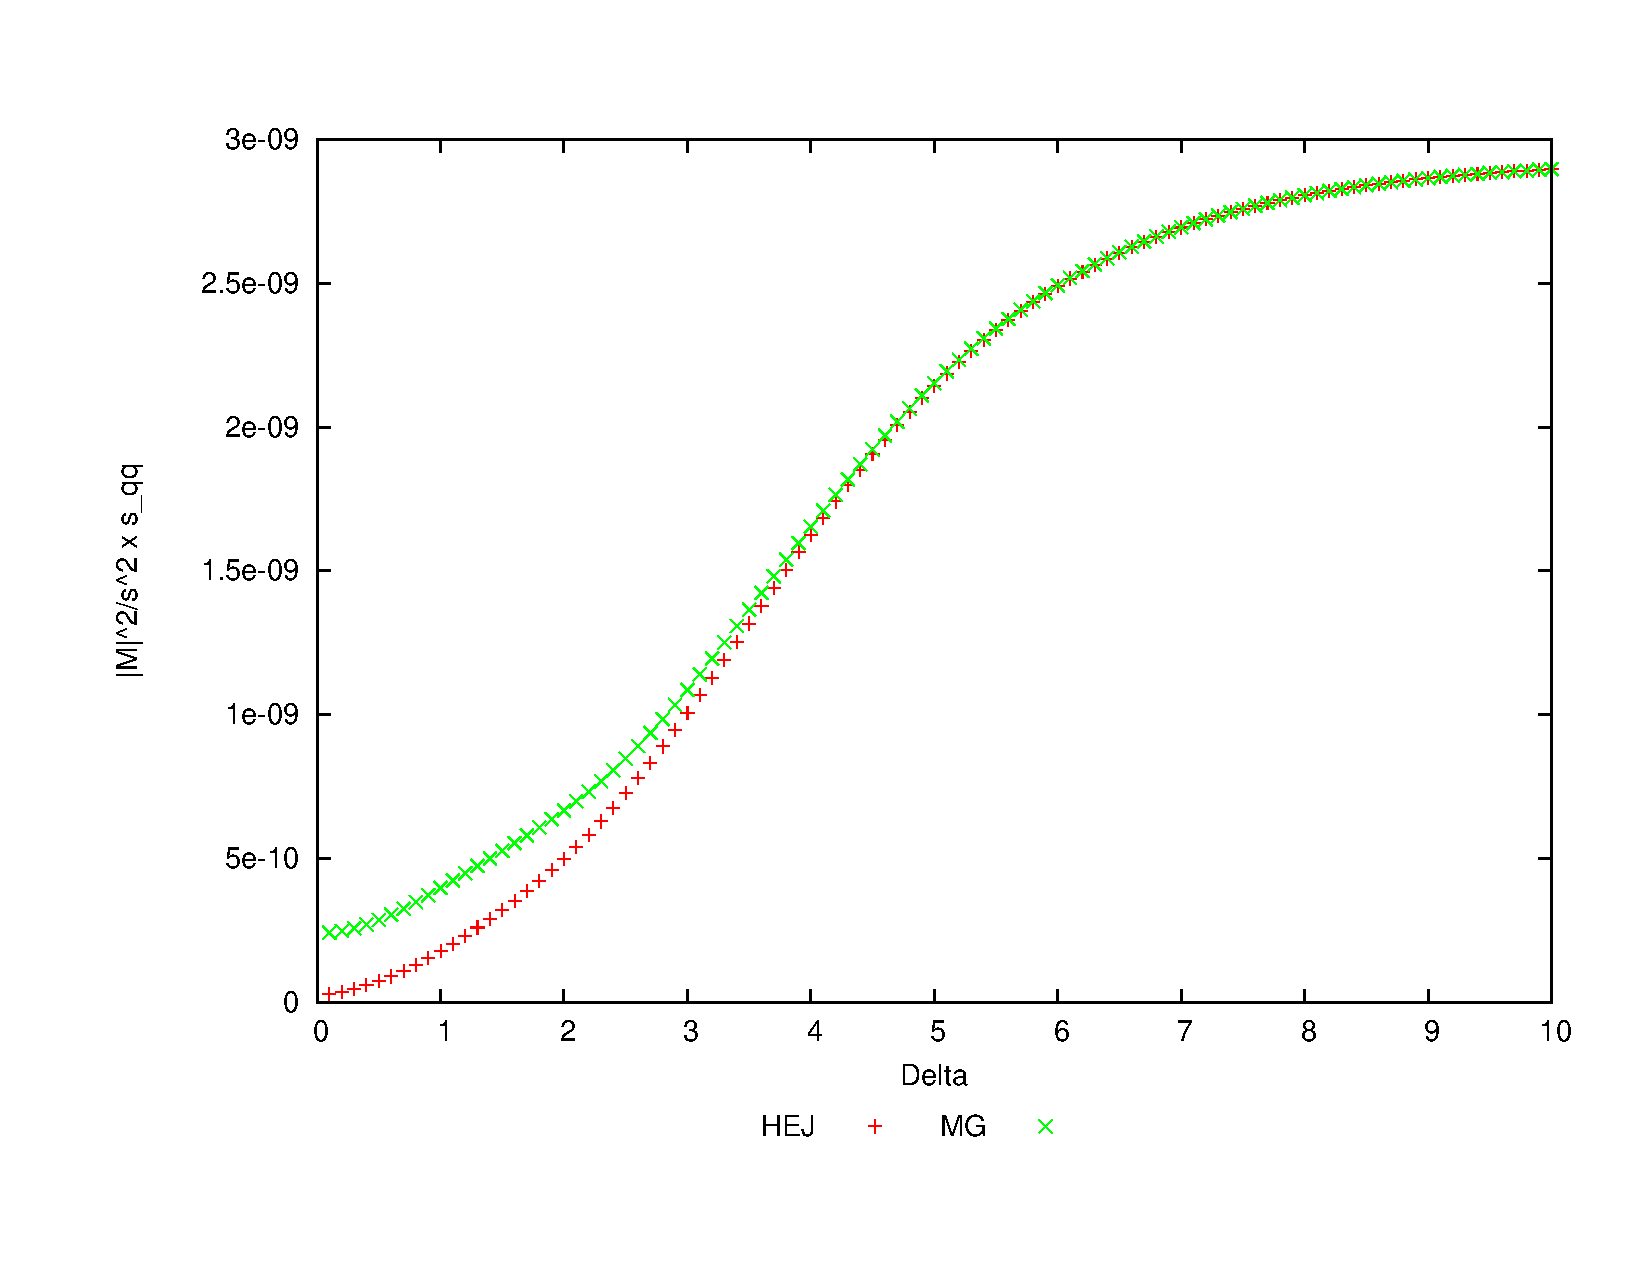
\includegraphics[scale=0.47]{Images/gg_gqqxg_sqq_simplecf.pdf}
\caption{Effective vertex approach to the $gg \to gQ\bar{Q}g$ amplitude (red) compared to the full LO (green) multiplied by the invariant mass of the quark/anti-quark pair.}
\label{fig:gg_gqqg}
\end{figure}

Again, we conclude that the colour factor multiplication is sufficient to approximate the full leading order result. We therefore move on to discussing how extra gluon emissions are added to these amplitudes. Because of the factorisation properties of the High Energy Limit, so long as we assume the extra gluon emissions are far away in rapidity from the partons already in the amplitude, we can simply multiply in a Lipatov vertex, along with a colour factor and then dividing by additional $t$-channel poles that will appear. For the $qg \to qQ\bar{Q}$ case, this yields simply;

\begin{equation}
|M_{qg \to q...Q\bar{Q}}|^2 \sim |M_{qg \to qQ\bar{Q}}|^2 \times \prod_{i=1}^{n-3}  C_A \left(\frac{-V(q_i,q_{i+1}) \cdot V(q_i,q_{i+1})}{q_i^2} \right),
\end{equation}

where the set of dots represents the emission of $n-3$ gluons, with $n$ being the total number of final state partons. For the $qq' \to qQ\bar{Q}q'$ amplitude, we can either have the gluon emitted in rapidity between the most forward parton and the quark/anti-quark pair or between the pair and the most backward parton;

\begin{equation}
\begin{split}
|M_{qq' \to q...Q\bar{Q}...q'}|^2 &= |M_{qq' \to qQ\bar{Q}q'}|^2 \times \prod_{i=1}^{n_a} C_A \left(\frac{-V(q_i,q_{i+1}) \cdot V(q_i,q_{i+1})}{q_{i+1}^2} \right) \\
&\times \prod_{j=n_a+2}^{n-2} C_A \left(\frac{-V(q_j,q_{j+1}) \cdot V(q_j,q_{j+1})}{q_j^2} \right),
\end{split}
\end{equation}

where $n_a$ is the number of gluons more forward in rapidity than the quark/anti-quark pair. We take the simple case of emitting one extra gluon and again compare to the full leading order result to check that the argument we employ holds. In figure \ref{fig:qg_qqq_emis} we plot our effective description for the $qg \to qgQ\bar{Q}$ amplitude with an extra gluon emission and compare with the leading order result. The momenta we use are the same as the momenta in equation \ref{eqn:4jetmom}. 

\begin{figure}[H]
\centering
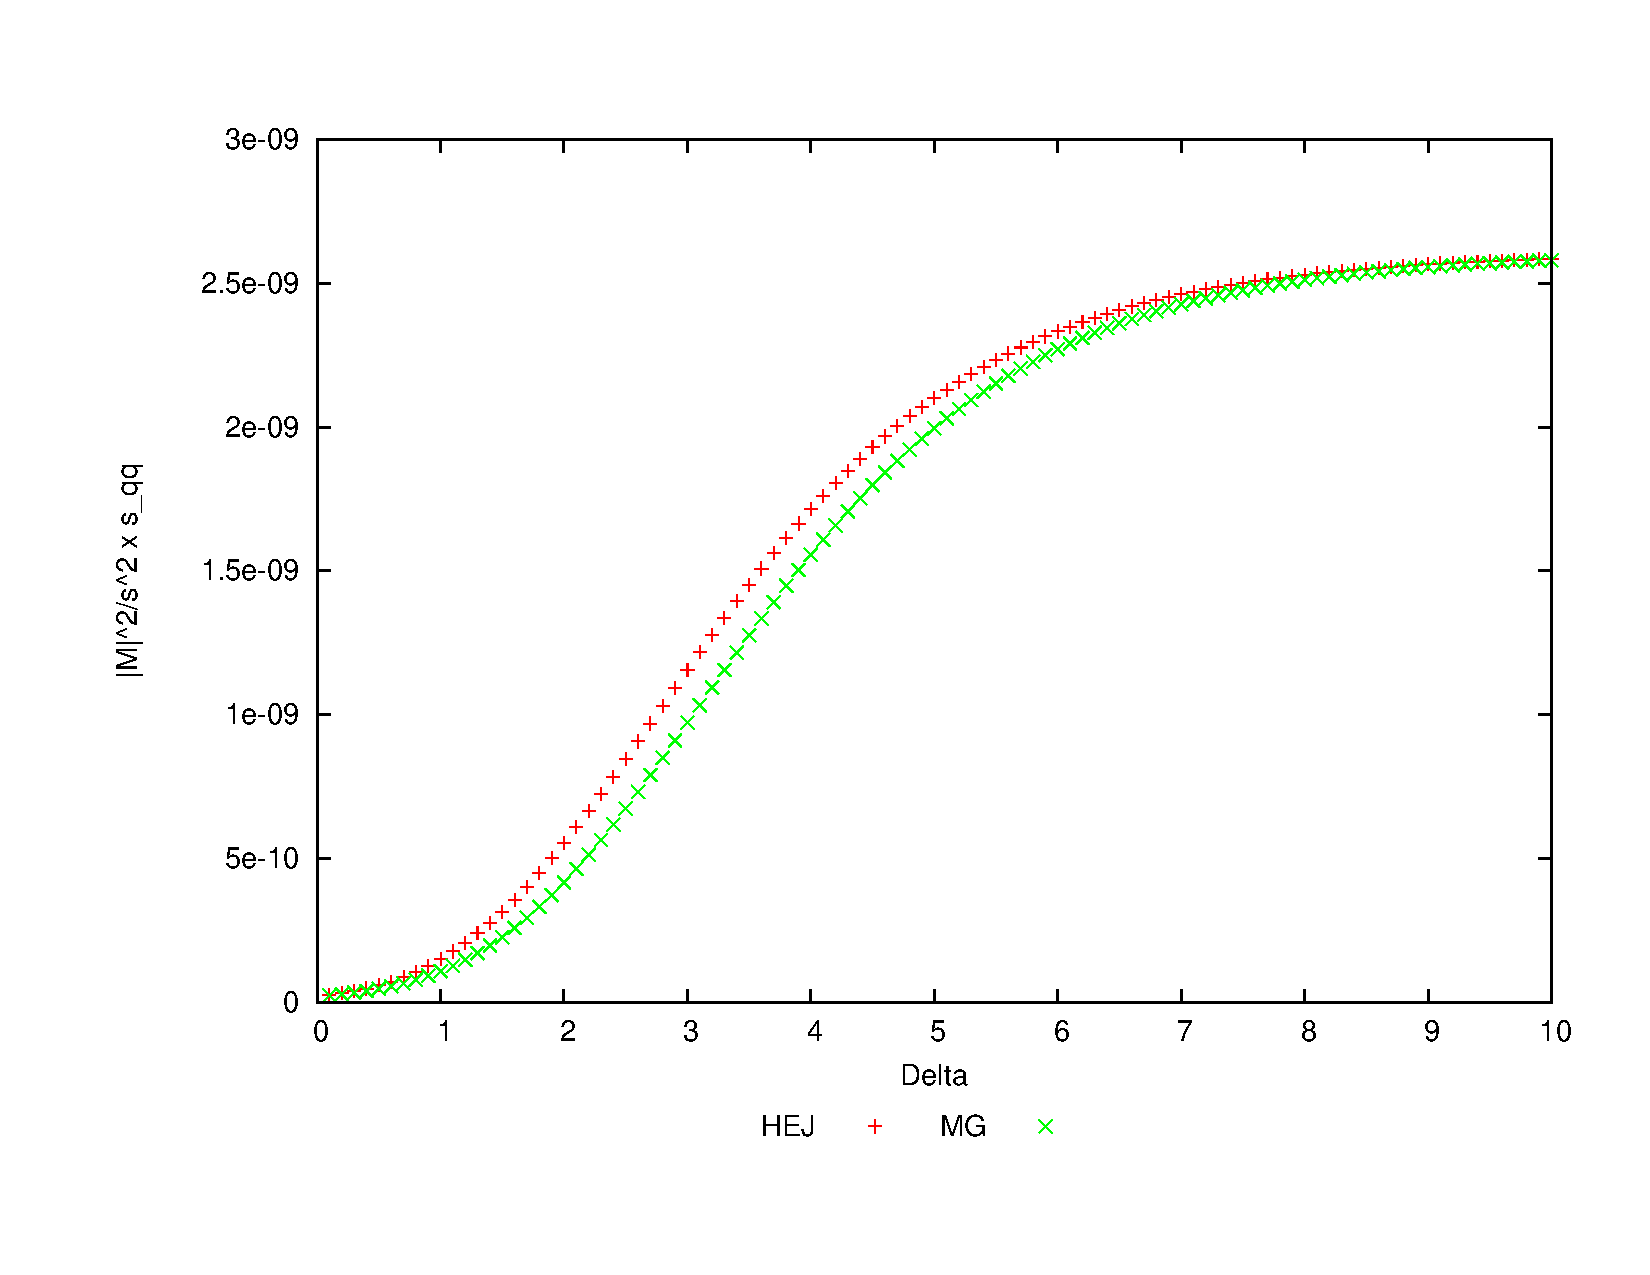
\includegraphics[scale=0.45]{Images/qg_qgQQx_sqq.pdf}
\caption{Effective vertex approach to the $qg \to qgQ\bar{Q}$ amplitude (red) compared to the full LO (green) multiplied by the invariant mass of the quark/anti-quark pair.}
\label{fig:qg_qqq_emis}
\end{figure}

For the case of the central $q\bar{q}$ emission plus an extra gluon emission, we employ the following set of five jet momenta;

\begin{equation}
\begin{split}
p_1 & = (40 \cosh(\Delta), 0, 40, 40 \sinh(\Delta)), \\
p_2 & = (40 \cosh(\Delta/2), -40, 0, 40 \sinh(\Delta/2)), \\
p_3 & = (80 \sqrt{2}, 80, -80, 0), \\
p_4 & = (40 \cosh(-\Delta/2), -40, 0, 40 \sinh(-\Delta/2)), \\
p_5 & = (40 \cosh(-\Delta), 0, 40, 40 \sinh(-\Delta)). 
\end{split}
\end{equation}

In figure \ref{fig:central_gfor} we plot the result for when the gluon is more forward in rapidity than the $q\bar{q}$ pair and in \ref{fig:central_gfor} we have the result for when it is emitted more backward in rapidity. All three of these latest figures show the reasonable agreement with the full result. 

\begin{figure}[H]
\centering
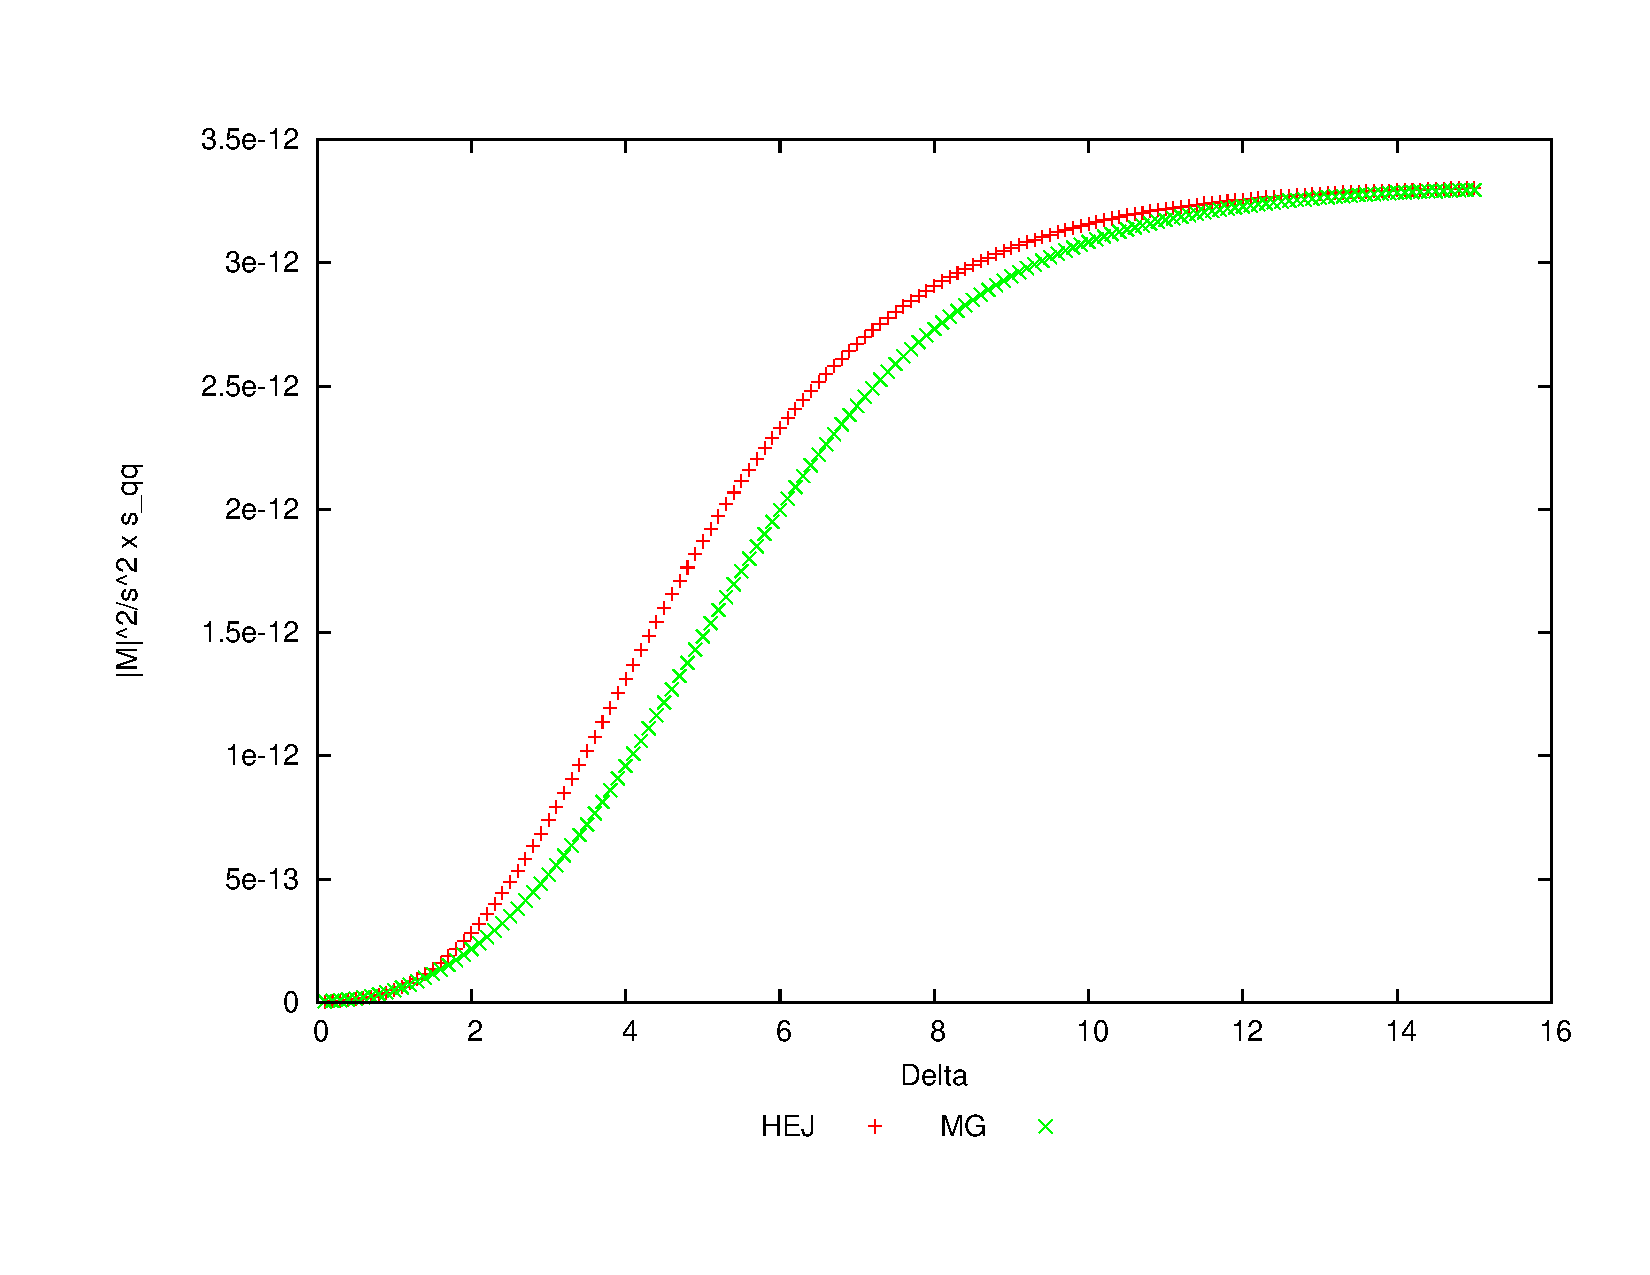
\includegraphics[scale=0.44]{Images/qQ_qgqqxQ_sqq.pdf}
\caption{Effective vertex approach to the $qq' \to qgQ\bar{Q}q'$ amplitude (red) compared to the full LO (green) multiplied by the invariant mass of the quark/anti-quark pair.}
\label{fig:central_gfor}
\end{figure}

\begin{figure}[H]
\centering
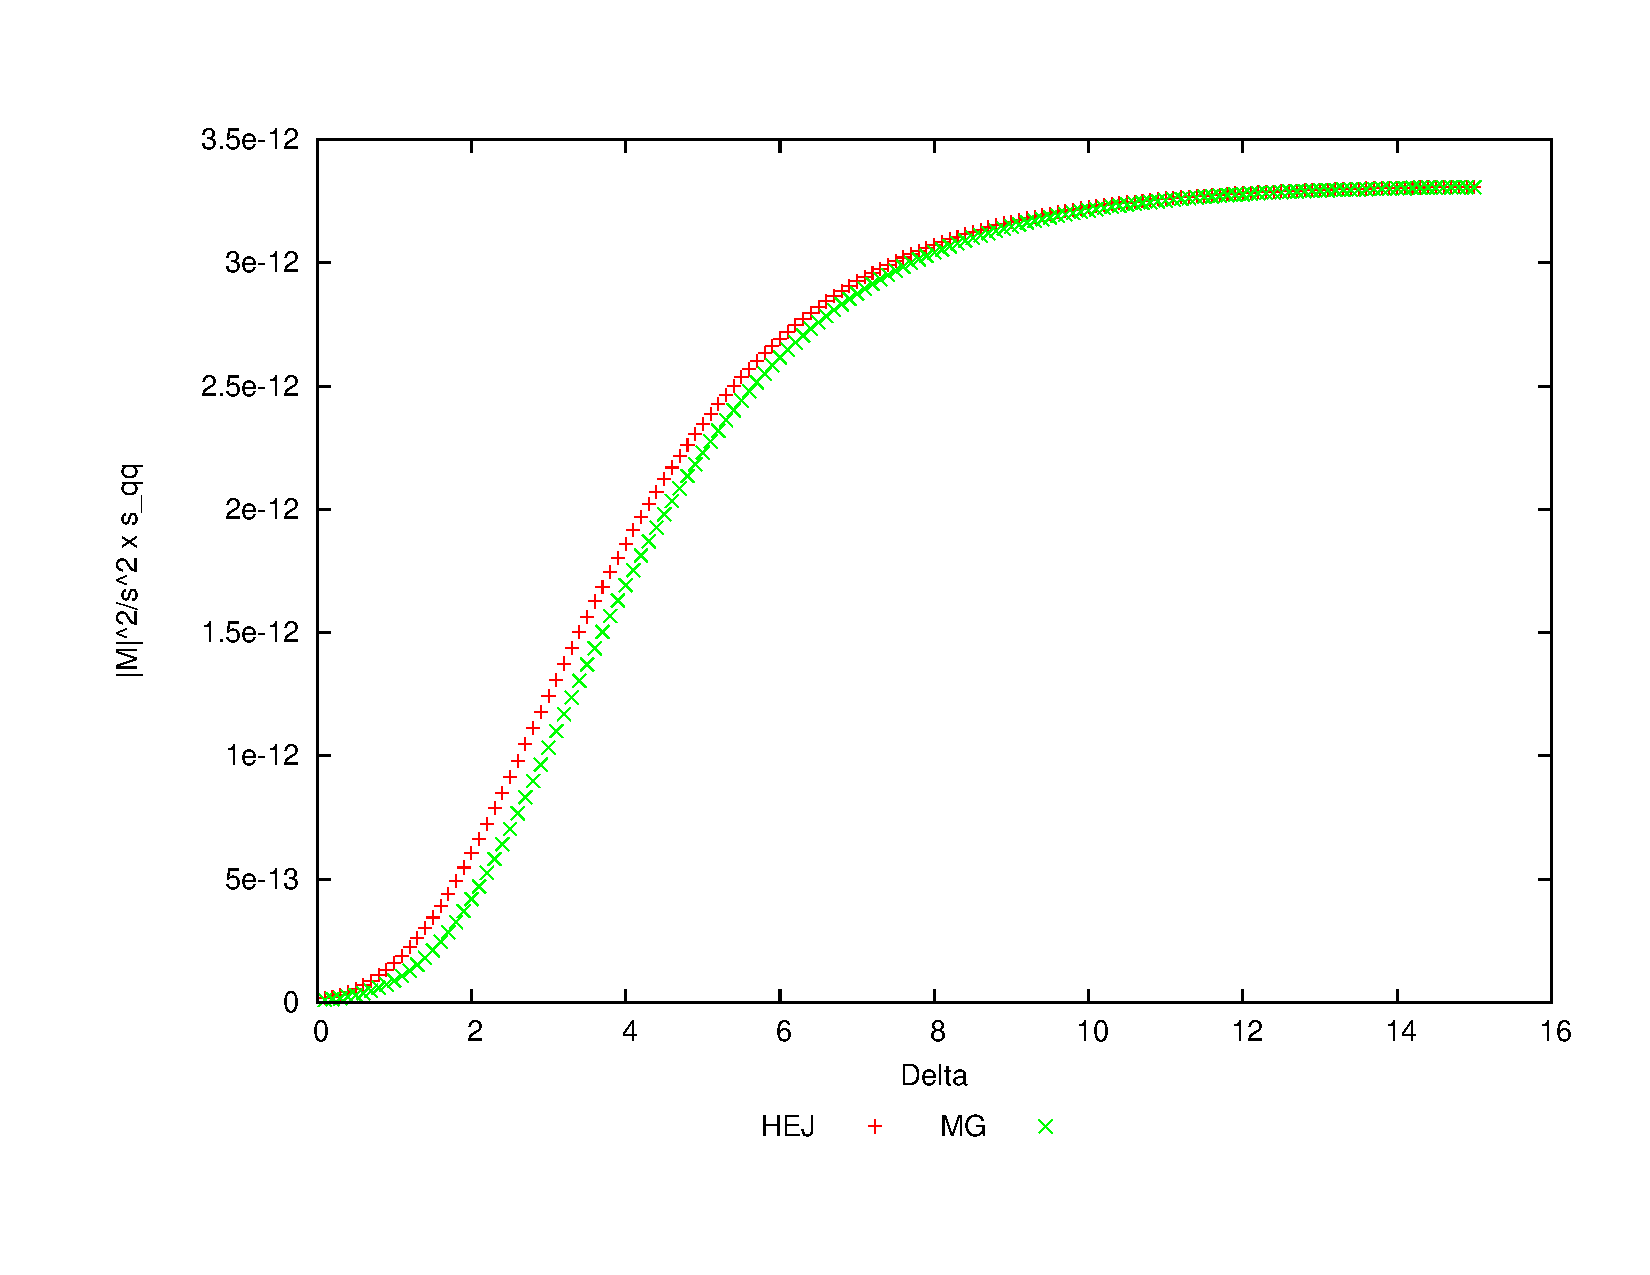
\includegraphics[scale=0.44]{Images/qQ_qqqxgQ_sqq.pdf}
\caption{Effective vertex approach to the $qq' \to qQ\bar{Q}gq'$ amplitude (red) compared to the full LO (green) multiplied by the invariant mass of the quark/anti-quark pair.}
\label{fig:central_gback}
\end{figure}

\section{Computational Aspects}
%\todo{removing from nonFKL, generating all possible processes, making sure matching is done consistently} 
The plots of the last section all served to convince that the derived amplitudes behaved as expected. The next step is to include them in the full HEJ program correctly. This is a very significant change to the codebase that requires the modification of many files and so a `branch' of the code base was created so that all work can be done independent of other projects going on in the collaboration. Once everything is done and checked, the branch can be `merged' back into the main development code base in a way that does not disrupt any other work done there since the branch was created. The points that need to be considered when adding these amplitudes in are as follows;
\begin{enumerate}
\item{Correctly removing calls to fixed order non-FKL processes if they are now to be included in the resummation. For example, the code already contains a call to the $qg \to qQ\bar{Q}$ amplitude at leading order for matching purposes. We therefore need to remove calls to these particular subprocesses in that section of the code and we need to remove them only if the user specifies that they wish to include these processes in the resummation (although it will become default for HEJ to include them). }
\item{Ensuring that all possible processes are generated. Since the HEJ program is a Monte Carlo program, we must ensure that all of these extra NLL processes are `picked'. Since we are requiring a leading order matching, one consideration is that an NLL process should not be picked if the event will not be clustered into at least three jets. Also, given a set number of final state partons and a central $q\bar{q}$ emission, we must make sure that all positions of that emission along that chain are considered. Another point is that the rapidity ordering of the $q\bar{q}$ pair can be either way around and we must include both orderings. Failure to do any of this correctly will mean that the program will be artificially removing physics that we know is there.}
\item{Checking that the leading order matching at the jet level for the NLL processes is done consistently. For example, imagine we generate a central $q\bar{q}$ emission at the parton level and choose partons $p_i$ and $p_j$ for the pair, where $p_i$ is more forward than and next to $p_j$ in rapidity. In order to properly implement the matching, we require that these cluster into two different jets, $p_i \to j_i$ and $p_j \to j_j$, whereby $j_i$ is more forward than and next to $j_j$ in rapidity. Because of how the clustering works, it is not at all guaranteed that the jets will preserve this rapidity ordering and furthermore that these jets are even still next to each other in rapidity in the chain. All these considerations must be carefully checked. }
\end{enumerate} 
It is absolutely crucial that all of these points are properly addressed and checked and so such a task is necessarily time consuming. After validating these steps by comparisons to old code with certain restraints, we can be confident that everything works as it should. %\todo{Include some comparison here?}
\section{Results}
%\todo{Distributions, revisits to previous analyses with these effects added in, etc} 
One advantage of now being able to resum these partonic subprocesses and unordered events is that it means we have a reduced reliance on fixed order matching codes. Before, all process that were 'non-FKL' had to be included via ta leading order matching. We have shown here that some of these non-FKL process can themselves be resummed and therefore we no longer need to include these processes in the fixed order part. Figure \ref{fig:fklmigration} graphically shows the difference this makes. An analysis was run whereby we require at least three jets in the final state and the cross section broken down into the contribution coming from the resummation and the fixed order. It is desirable if the red line (the resummed contribution) is as close to the black line (the total contribution) as possible and it is clear from this plot that the addition of these partonic subprocesses is helping that in a significant way, reducing the relative contribution of the fixed order processes by a large fraction.  

\begin{figure}[t] 
\centering
\subfloat{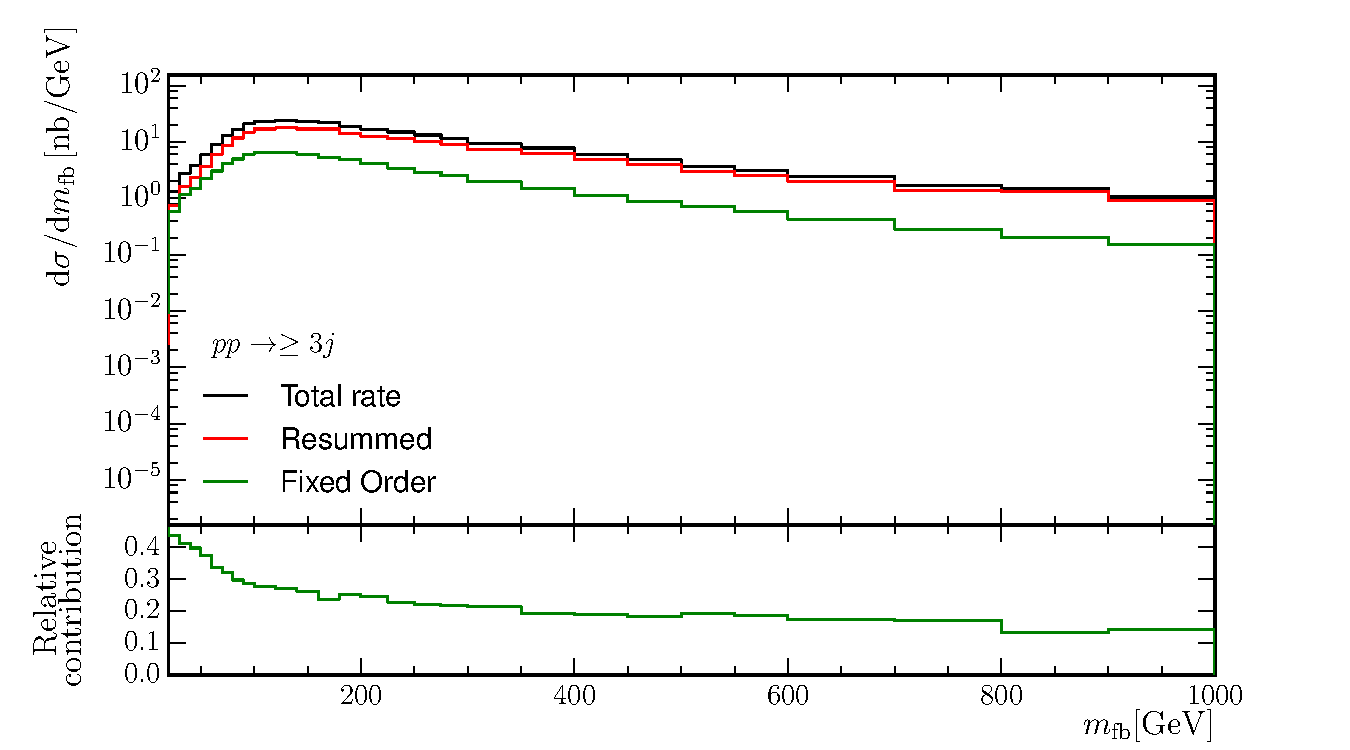
\includegraphics[scale=0.75]{Images/mfb_3jinc_bare_breakdown.pdf}} \\
\subfloat{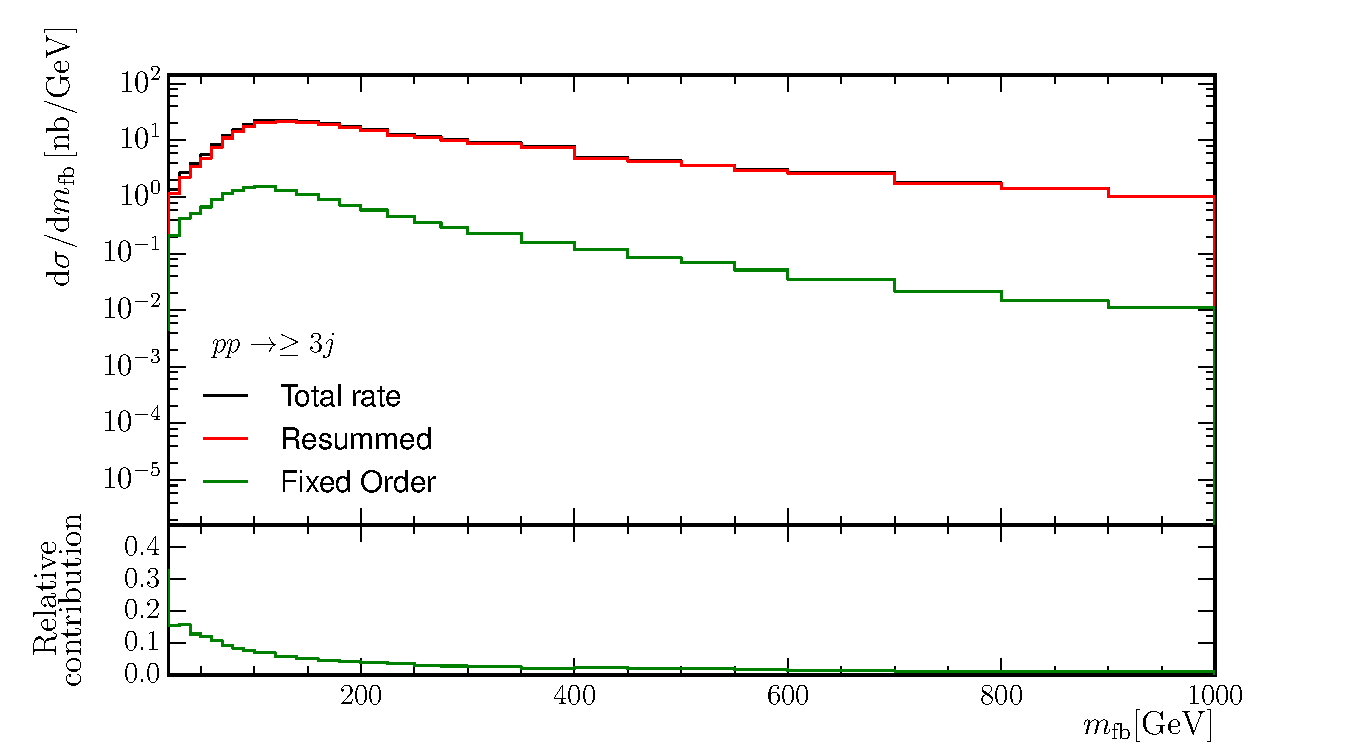
\includegraphics[scale=0.75]{Images/mfb_3jinc_resummed_breakdown.pdf}}
\caption{A breakdown of contributing parts to the jet cross section before (top) and after (bottom) implementing the effective vertex description of the new partonic subprocesses and the unordered events, in bins of the invariant mass between the most forward and backward jets.}
\label{fig:fklmigration}
\end{figure}
%\todo{Label this diagram better. Add new ones from NLL paper?}
We can also revisit the predictions for previous analyses HEJ was involved him and investigate how these new additions help whilst comparing with real data. For example, in an ATLAS study of dijet production with a central jet veto \cite{Aad2011}. One interesting plot is figure 6 of that paper, which is that of the average number of jets in the `gap', defined as the rapidity region between the dijet system which in this case is given by the two highest $p_T$ jets in a event. There are a total of four different lines which correspond to different rapidity slices shwon in figure \ref{fig:veto}. From the top; $4 \leq \Delta y < 5$, $3 \leq \Delta y < 4$, $2 \leq \Delta y < 3$ and $1 \leq \Delta y < 2$. In order to differentiate them on the graph, these lines are moved up by $3,2,1$ and $0$ respectively. The $x$-axis is $\bar{p}_t$, which is the average of the dijet system's transverse momenta. For the high energy limit HEJ considers, we should not expect this to be a good variable to plot in; the limit depends on all transverse scales being roughly the same order. At high average $p_T$, we can very easily construct a large $p_T$ hierarchy. This is indeed reflected at the right hand side of the figure. It was noted that the analysis might have been better performed by considering only the resummed part of the HEJ calculation, since it is this part that is going to give rise to gap jets. We therefore include both the full and resummed only lines in this figure. In the diagram on the top left, we see a considerable difference between these to lines. By adding these new processes, we make these lines essentially indistinguishable and at the same time capture more bins on the left hand side of the plots, which is the only place we can reasonably expect improvement. \\
\\
Furthermore, in a later dijet veto ATLAS analysis \cite{Aad2014}, it was observed that the predictions from the pure partonic HEJ needed to be interfaced with a parton shower in order to get the best description of the data. Although of course there are regions where a parton shower description is always going to be important, we can investigate to see if NLL effects can push the pure partonic line closer to the data by itself. For example, we can take a look at figure 3a of that paper. This figure plots the `Gap Fraction', defined as the ratio of the cross section for dijet events with no additional jets above a certain scale in the rapidity gap between the two jets to the cross section in total. Such an observable will clearly be sensitive to resummation effects, since we saw earlier that the rapidity gap plays a central role in the derivation of our amplitudes. In figure \ref{fig:newveto3a} we plot a comparison of data to four different HEJ runs, which correspond to the four different combinations of including/not including the unordered/sub-leading partonic processes corrections. For the same reasons as before, we plot both the resummed and full HEJ lines for comparison. The bottom right figure shows that the inclusion of both of these effects leads to a better description of the data everywhere, but in particular we `gain' a few extra bins at the left side of the figure.

\begin{figure}[t]
\centering
\subfloat[No NLL corrections.]{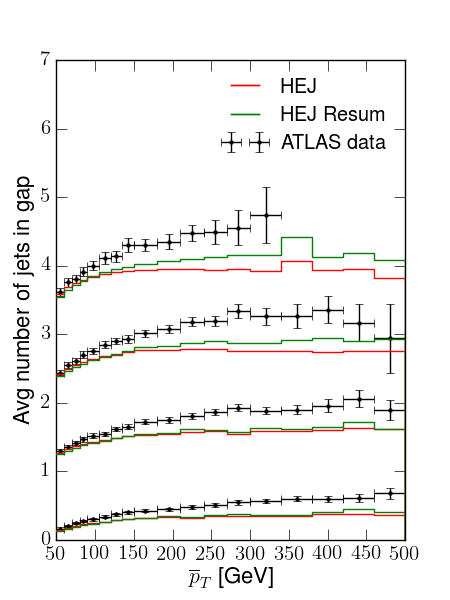
\includegraphics[scale=0.6]{Images/Veto_Plots/pf6_bare.png}}
\subfloat[Unordered corrections.]{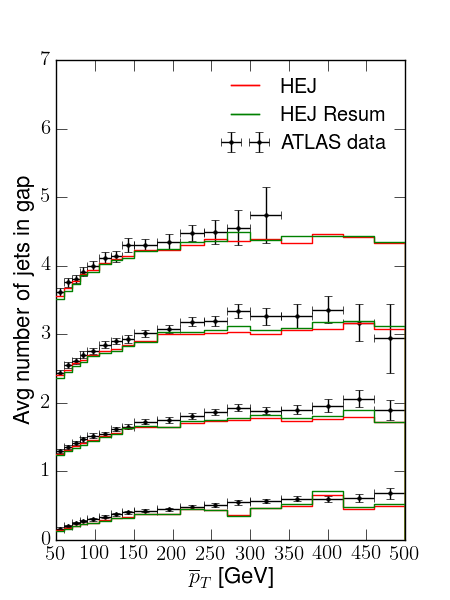
\includegraphics[scale=0.6]{Images/Veto_Plots/pf6_uno.png}} \\
\subfloat[Sub-leading partonic processes corrections.]{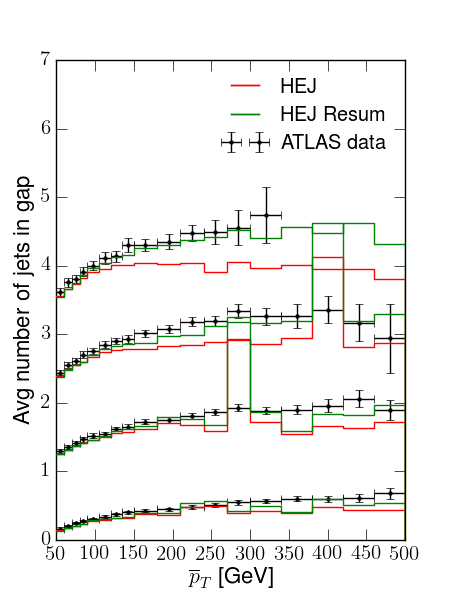
\includegraphics[scale=0.6]{Images/Veto_Plots/pf6_qqx.png}}
\subfloat[Both corrections.]{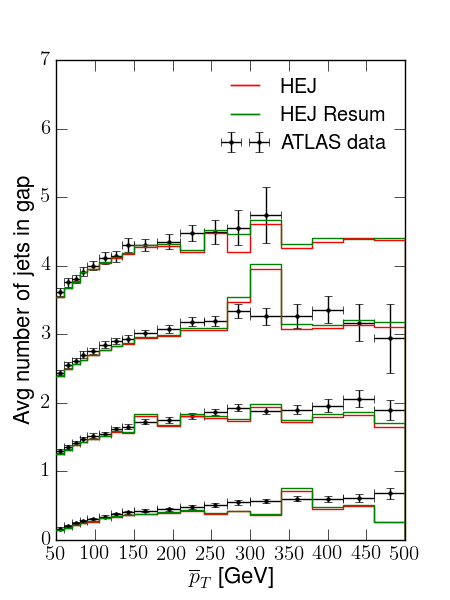
\includegraphics[scale=0.6]{Images/Veto_Plots/pf6_uno_qqx.png}}
\caption{Figure 6 of \cite{Aad2011} redone with corrections included. The red lines are the results from running the full HEJ program, the green if one only considers the resummed parts of the program and black points are the data. From the top let; no corrections, unordered corrections, sub-leading partonic processes corrections, both corrections. In the last figure, we see how these corrections mean that there is barely any distinction between `resummed' and `full' HEJ anymore.}
\label{fig:veto}
\end{figure}

\begin{figure}[t]
\centering
\subfloat[No NLL corrections.]{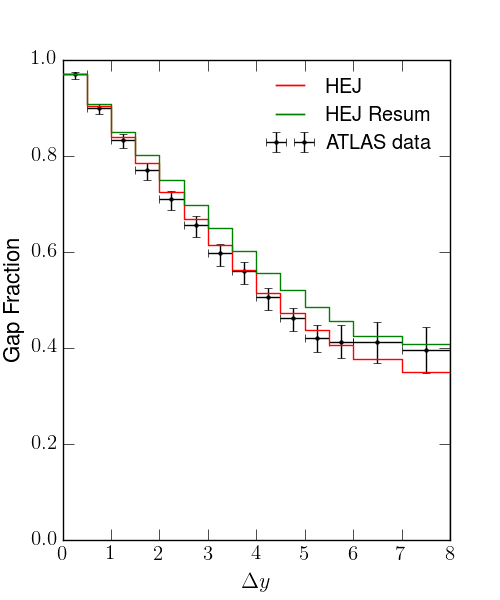
\includegraphics[scale=0.5]{Images/Veto_Plots/pf3a_bare.png}}
\subfloat[Unordered corrections.]{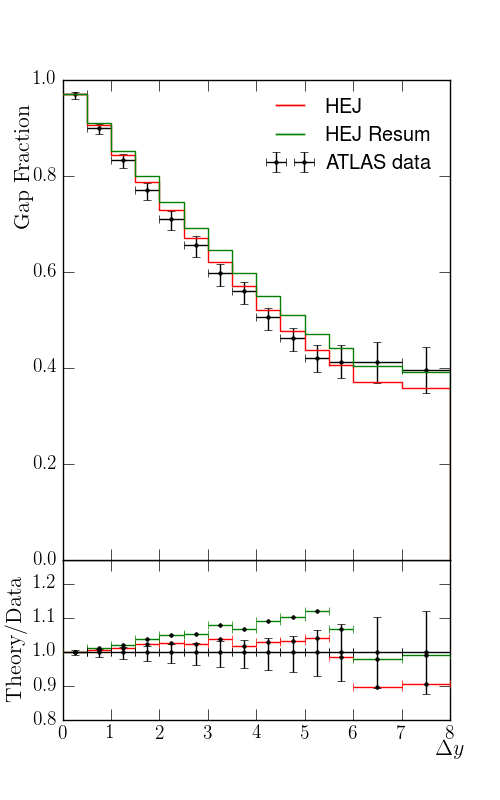
\includegraphics[scale=0.5]{Images/Veto_Plots/pf3a_uno.png}} \\
\subfloat[Sub-leading partonic processes corrections.]{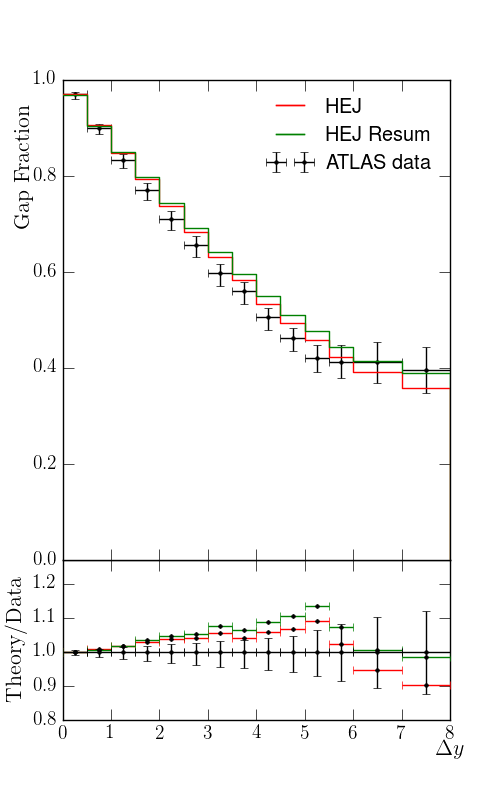
\includegraphics[scale=0.5]{Images/Veto_Plots/pf3a_qqx.png}}
\subfloat[Both corrections.]{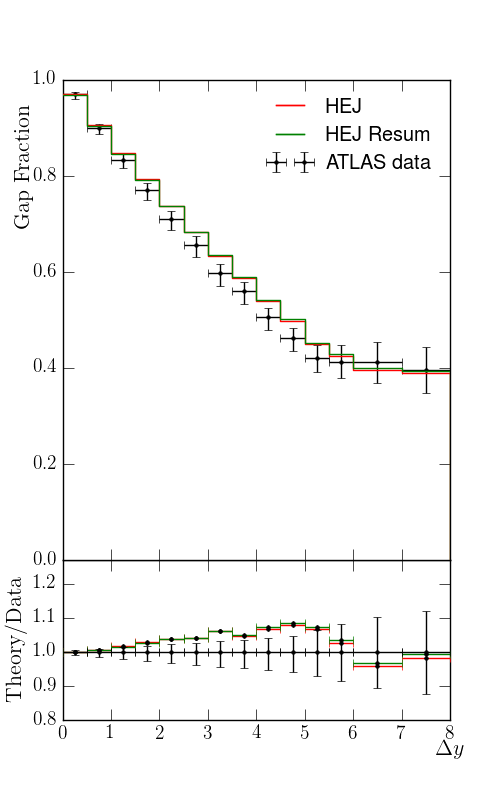
\includegraphics[scale=0.5]{Images/Veto_Plots/pf3a_uno_qqx.png}}
\caption{Figure 3a of \cite{Aad2014} redone with corrections included. The red lines are the results from running the full HEJ program, the green if one only considers the resummed parts of the program and black points are the data.}
\label{fig:newveto3a}
\end{figure}

Finally, we revisit a four-jet ATLAS analysis \cite{Aad2015}. This analysis is somewhat special in HEJ in that it includes matching for up to 5 jets in the final state (our usual approach is only up to 4). To compile the fixed order matrix elements for the 5 jet matching takes on the order of days and so is not practical to do generally. However, since this analysis specifically looks at four jet inclusive events, it was felt that it was necessary to have the matching to this level. In figure \ref{fig:4jet}, we look at figure 4 of that paper which is a measurement of the inclusive cross section binned in leading jet $p_T$. As mentioned before, $p_T$ is generally an observable that can be tricky to get right with the limit we consider, but we see here that if we make an inclusive measurement, we can describe the dat remarkably well. Once more, the addition of the new processes make this measurement even better. 

%\todo{Make last figure prettier - longer, less wide, better labelling}

\begin{figure}[t]
\centering
\subfloat[No NLL corrections.]{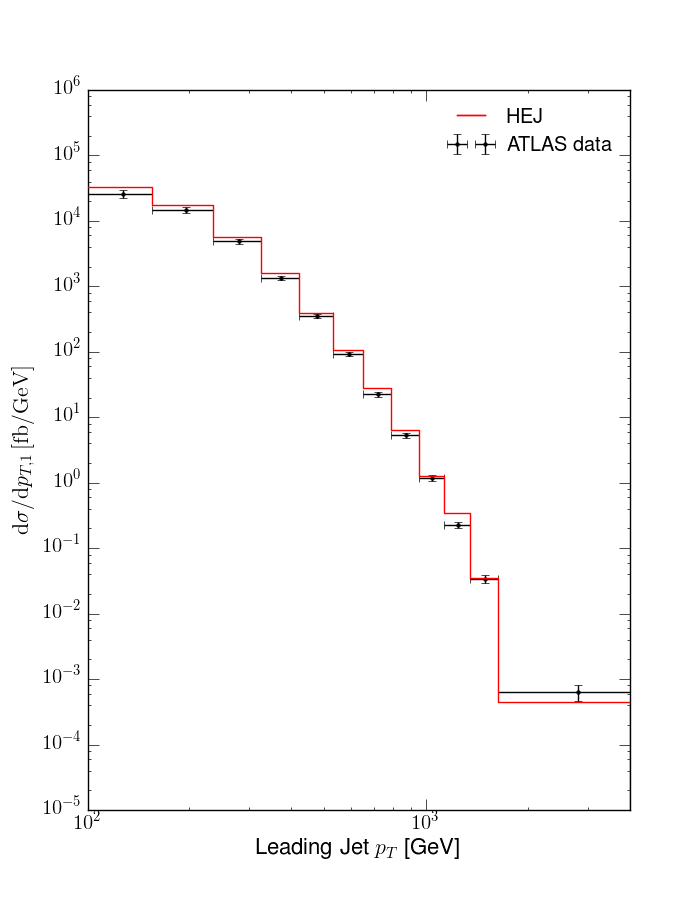
\includegraphics[scale=0.4]{Images/4j_plots/pf4_bare.png}}
\subfloat[Unordered corrections.]{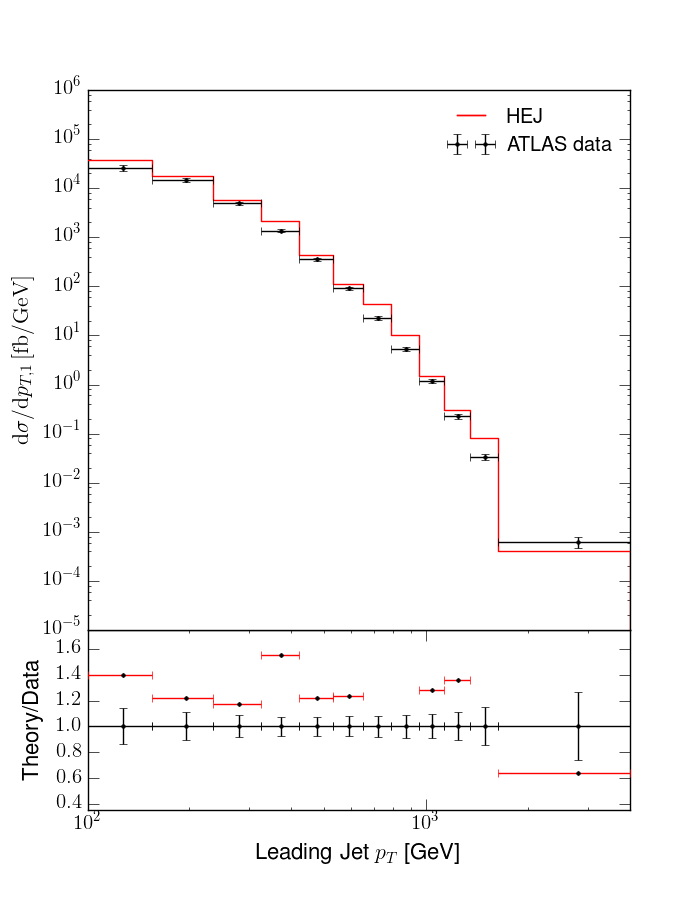
\includegraphics[scale=0.4]{Images/4j_plots/pf4_uno.png}} \\
\subfloat[Sub-leading partonic processes corrections.]{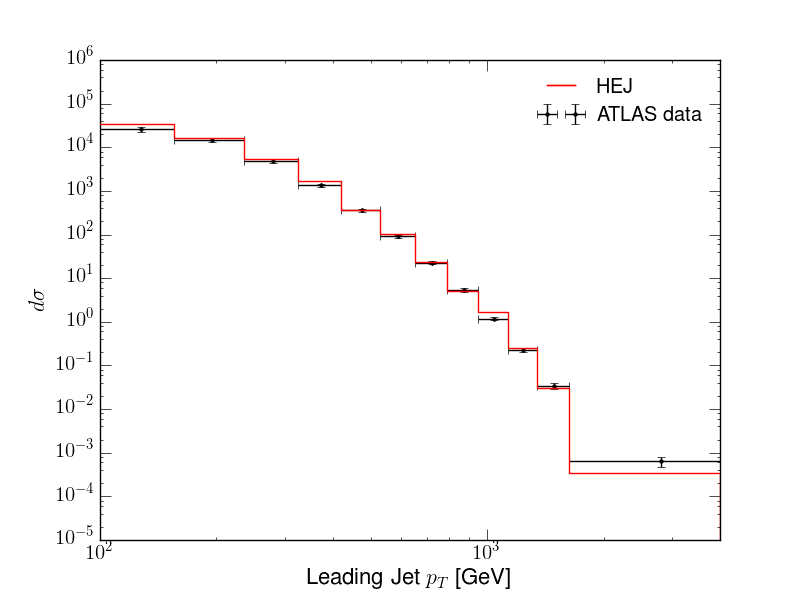
\includegraphics[scale=0.4]{Images/4j_plots/pf4_qqx.png}}
\subfloat[Both corrections.]{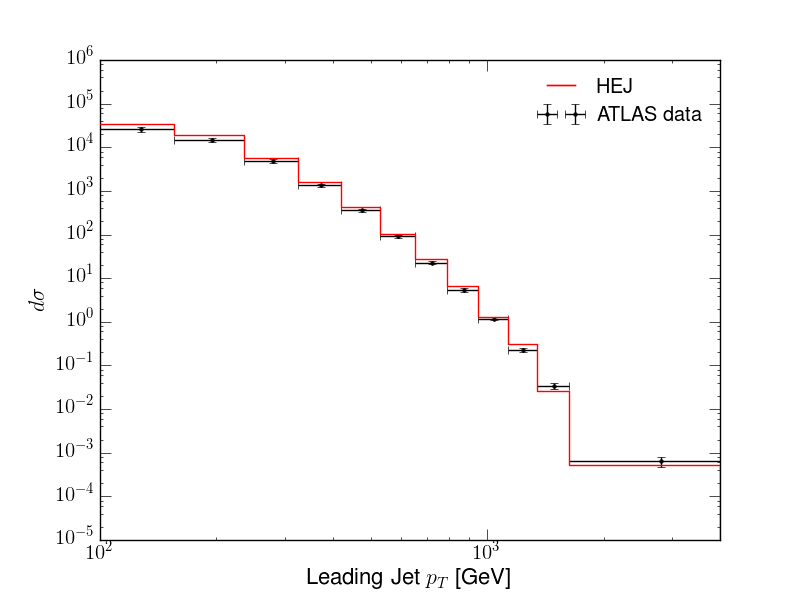
\includegraphics[scale=0.4]{Images/4j_plots/pf4_qqx_uno.png}}
\caption{Figure 4 of \cite{Aad2015} redone with corrections included and compared.}
\label{fig:4jet}
\end{figure}

%\todo{veto analysis plots, new veto analysis plots, 4 jet plots}
